%%____________________________________________________________________________||
\clearpage
\section{\texorpdfstring{\znunu\ + jets}{Zinv} background estimation}
\label{app:zinv}

\subsection{The ``transfer factor'' method}

\begin{figure}[!h]
  \centering
  \subfigure[Transfer factors as a function of (\njet,\nb) and \scalht.]{
    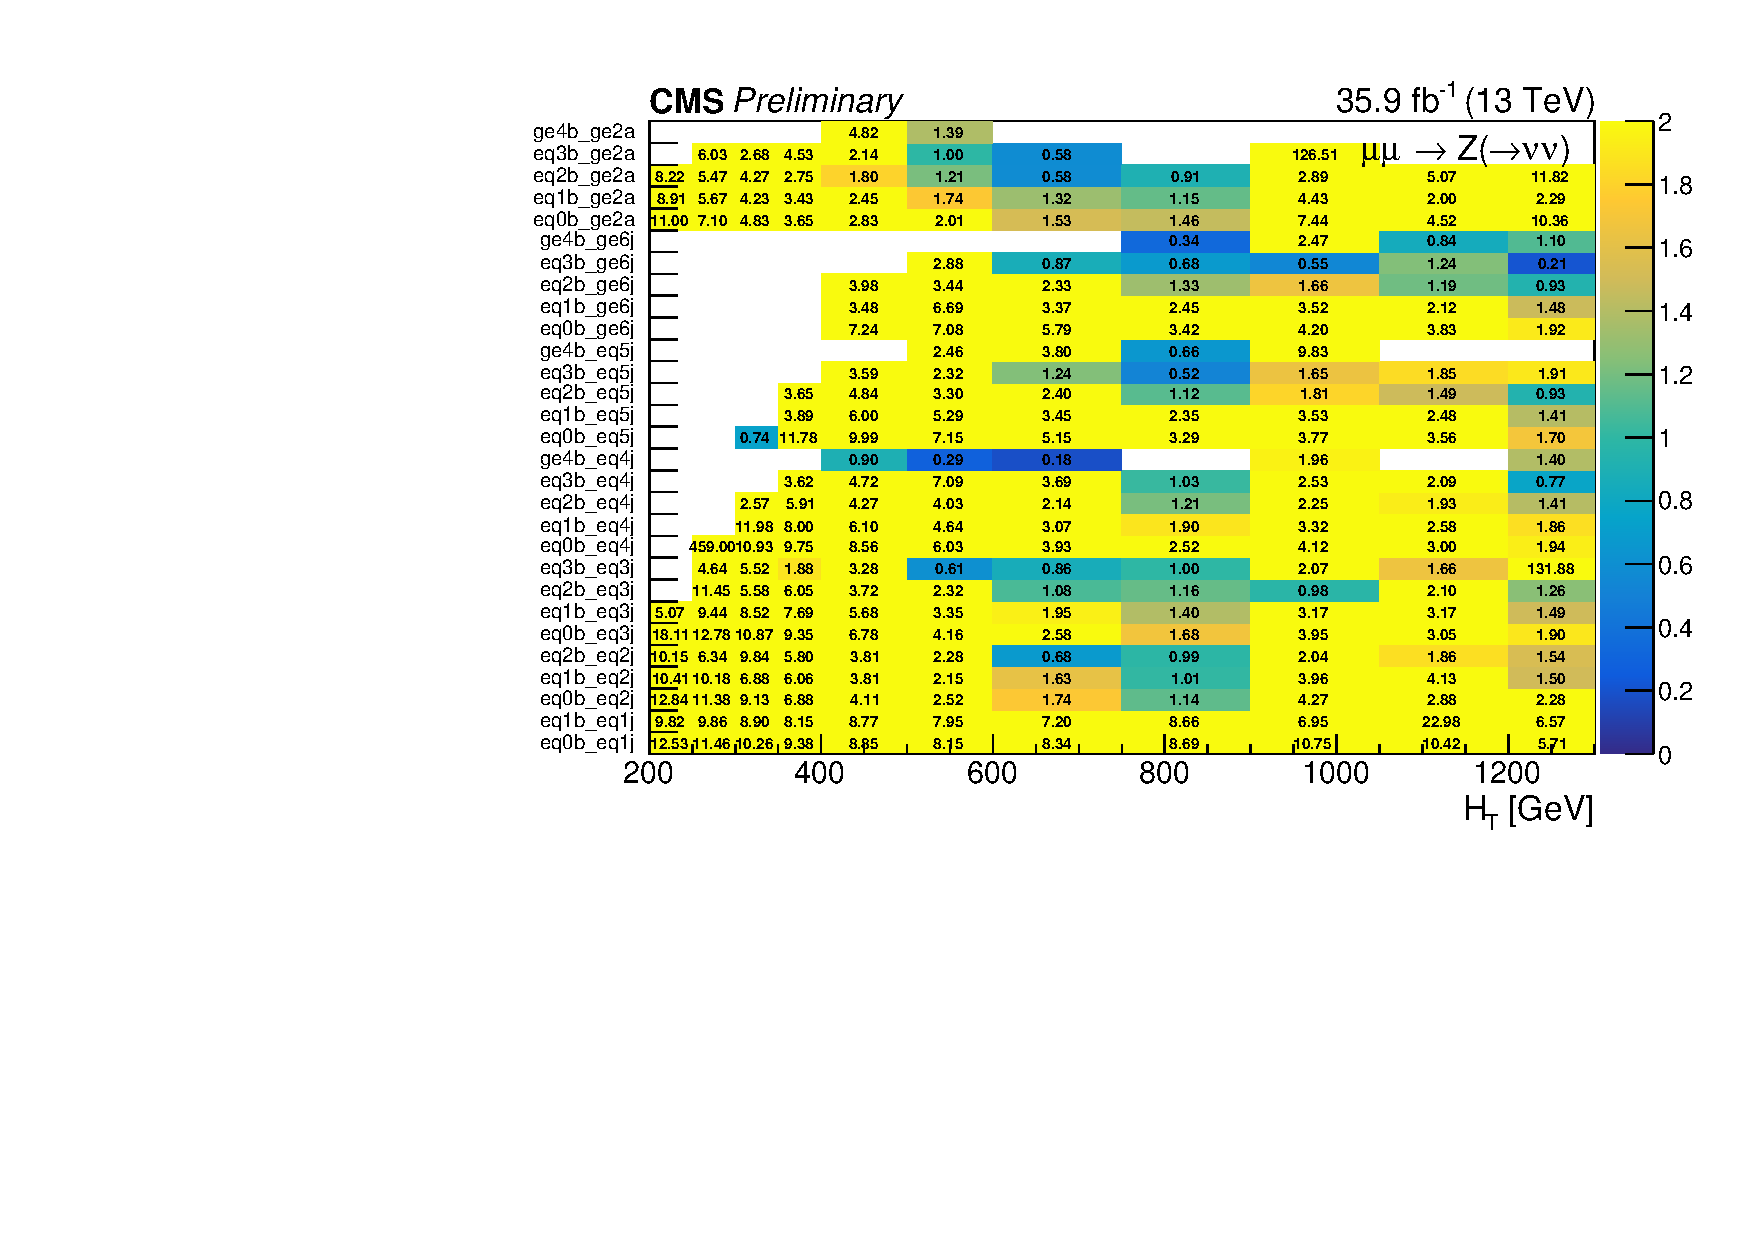
\includegraphics[width=0.5\textwidth]{figures/mcSystematics36p4fb/plots/tf_mumu_Zinv_2d_nominalUp.pdf}
  } \\
  \subfigure[Transfer factor as a function of \njet.]{
    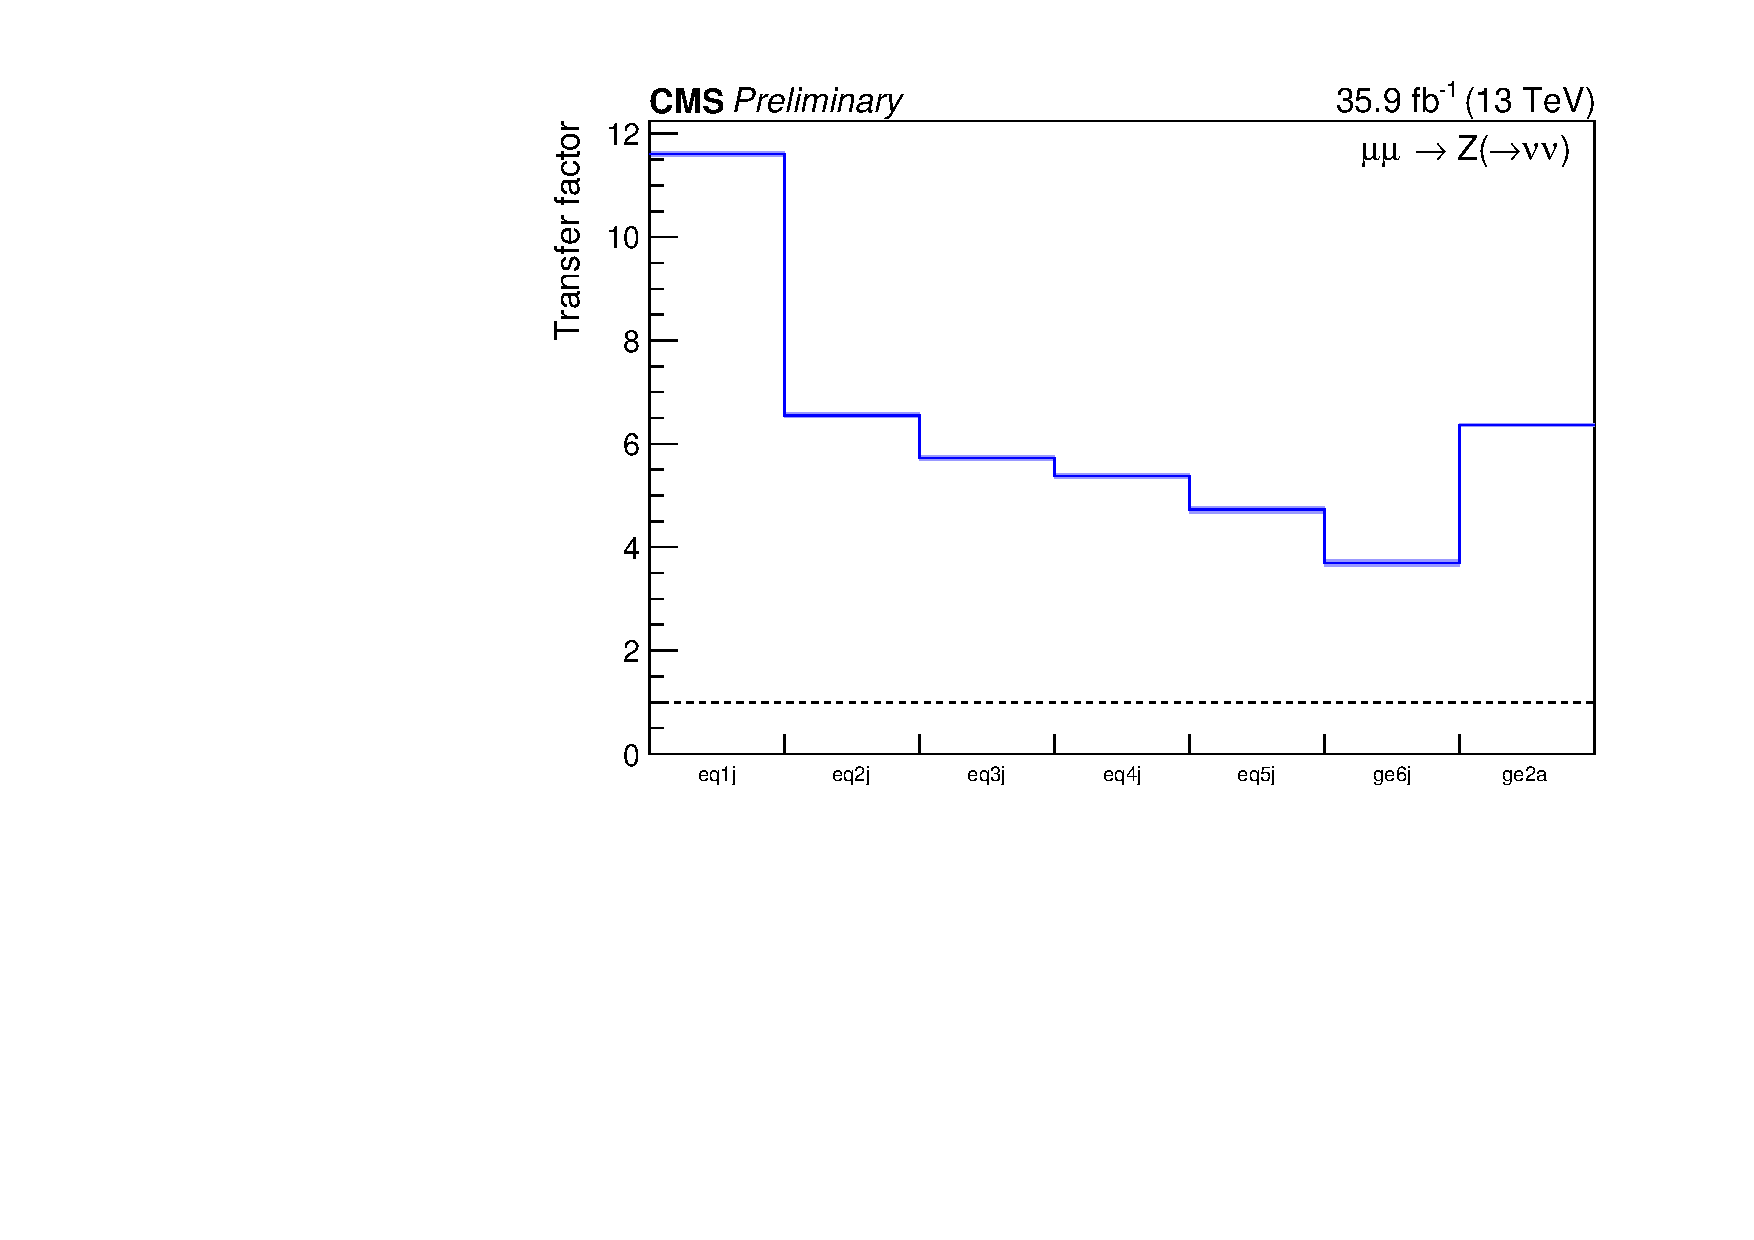
\includegraphics[width=0.5\textwidth]{figures/mcSystematics36p4fb/plots/tf_mumu_Zinv_njet_nominalUp.pdf}
  } ~
  \subfigure[Transfer factor as a function of \scalht.]{
    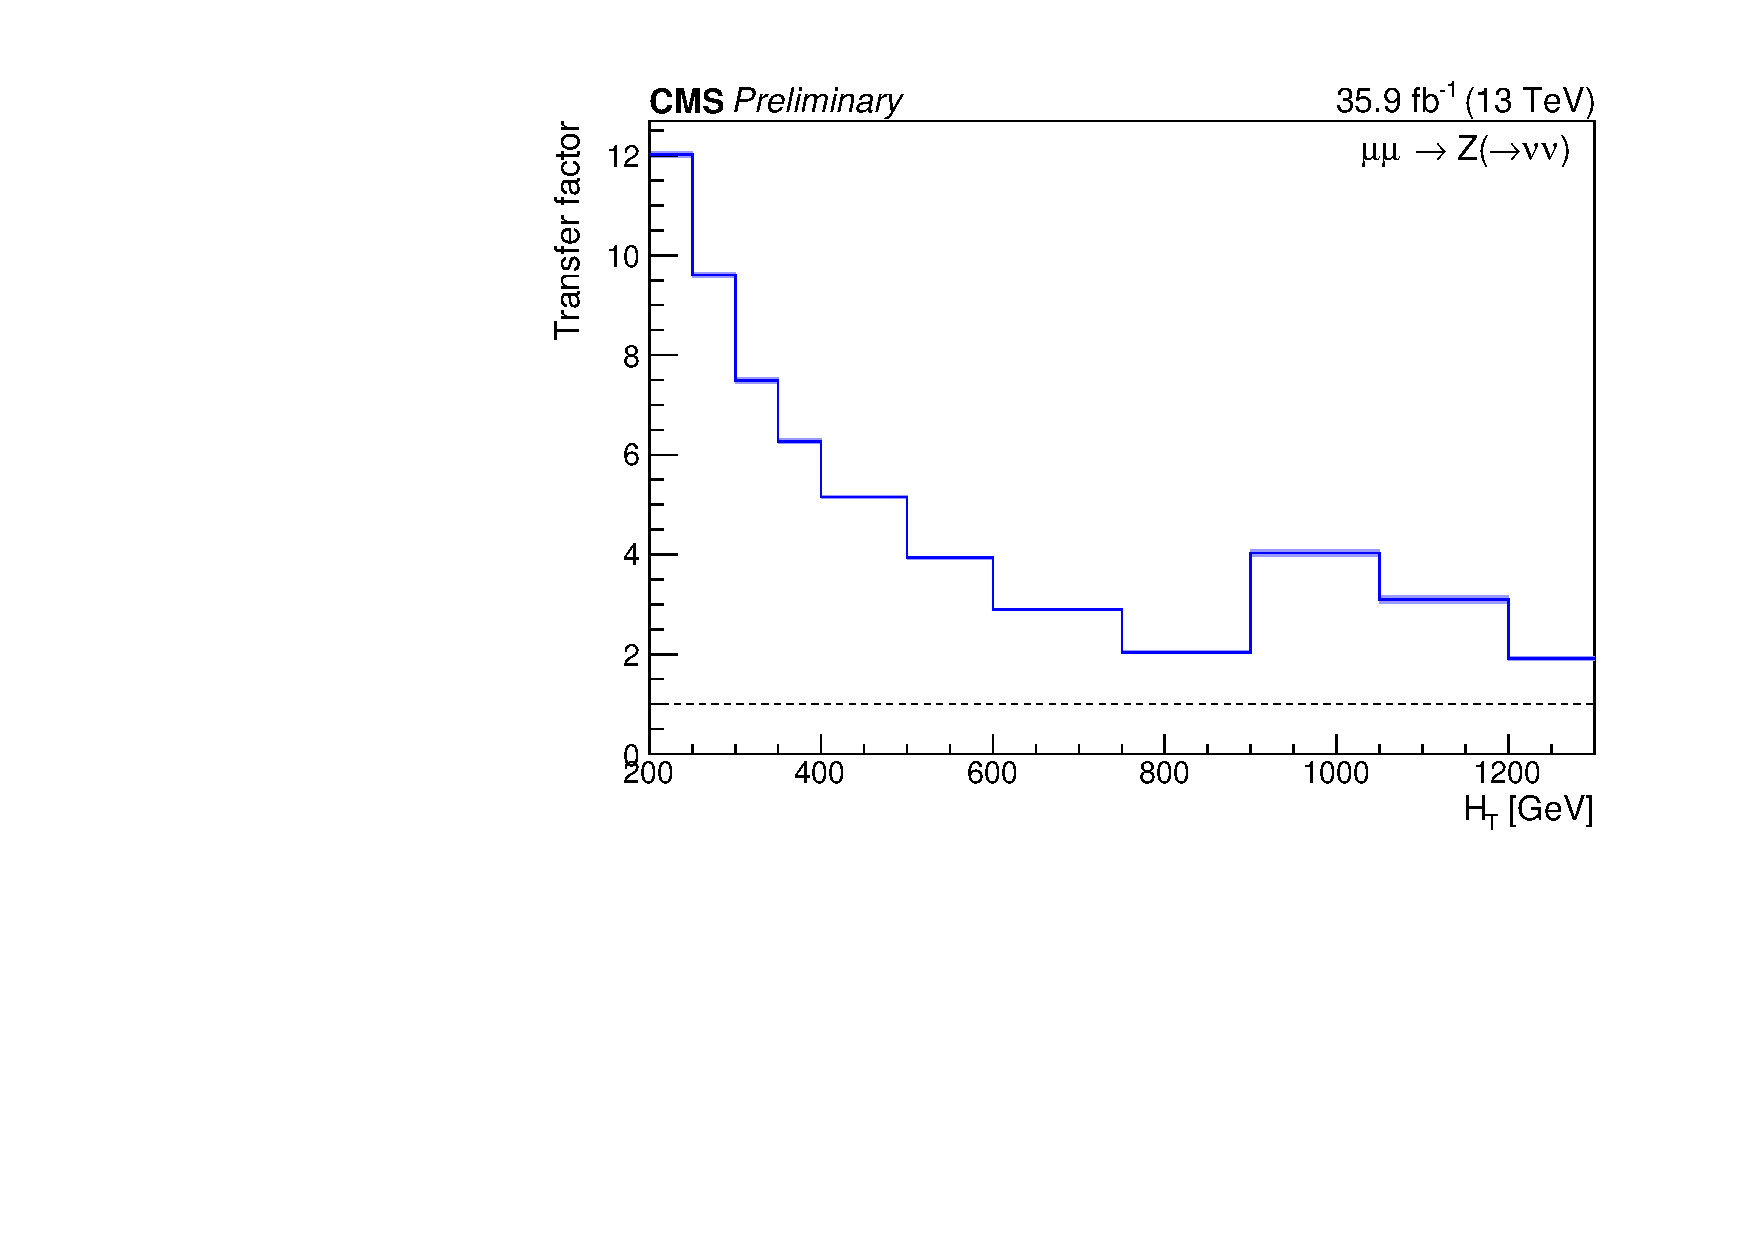
\includegraphics[width=0.5\textwidth]{figures/mcSystematics36p4fb/plots/tf_mumu_Zinv_ht_nominalUp.pdf}
  } \\
  \subfigure[Transfer factor as a function of \nb.]{
    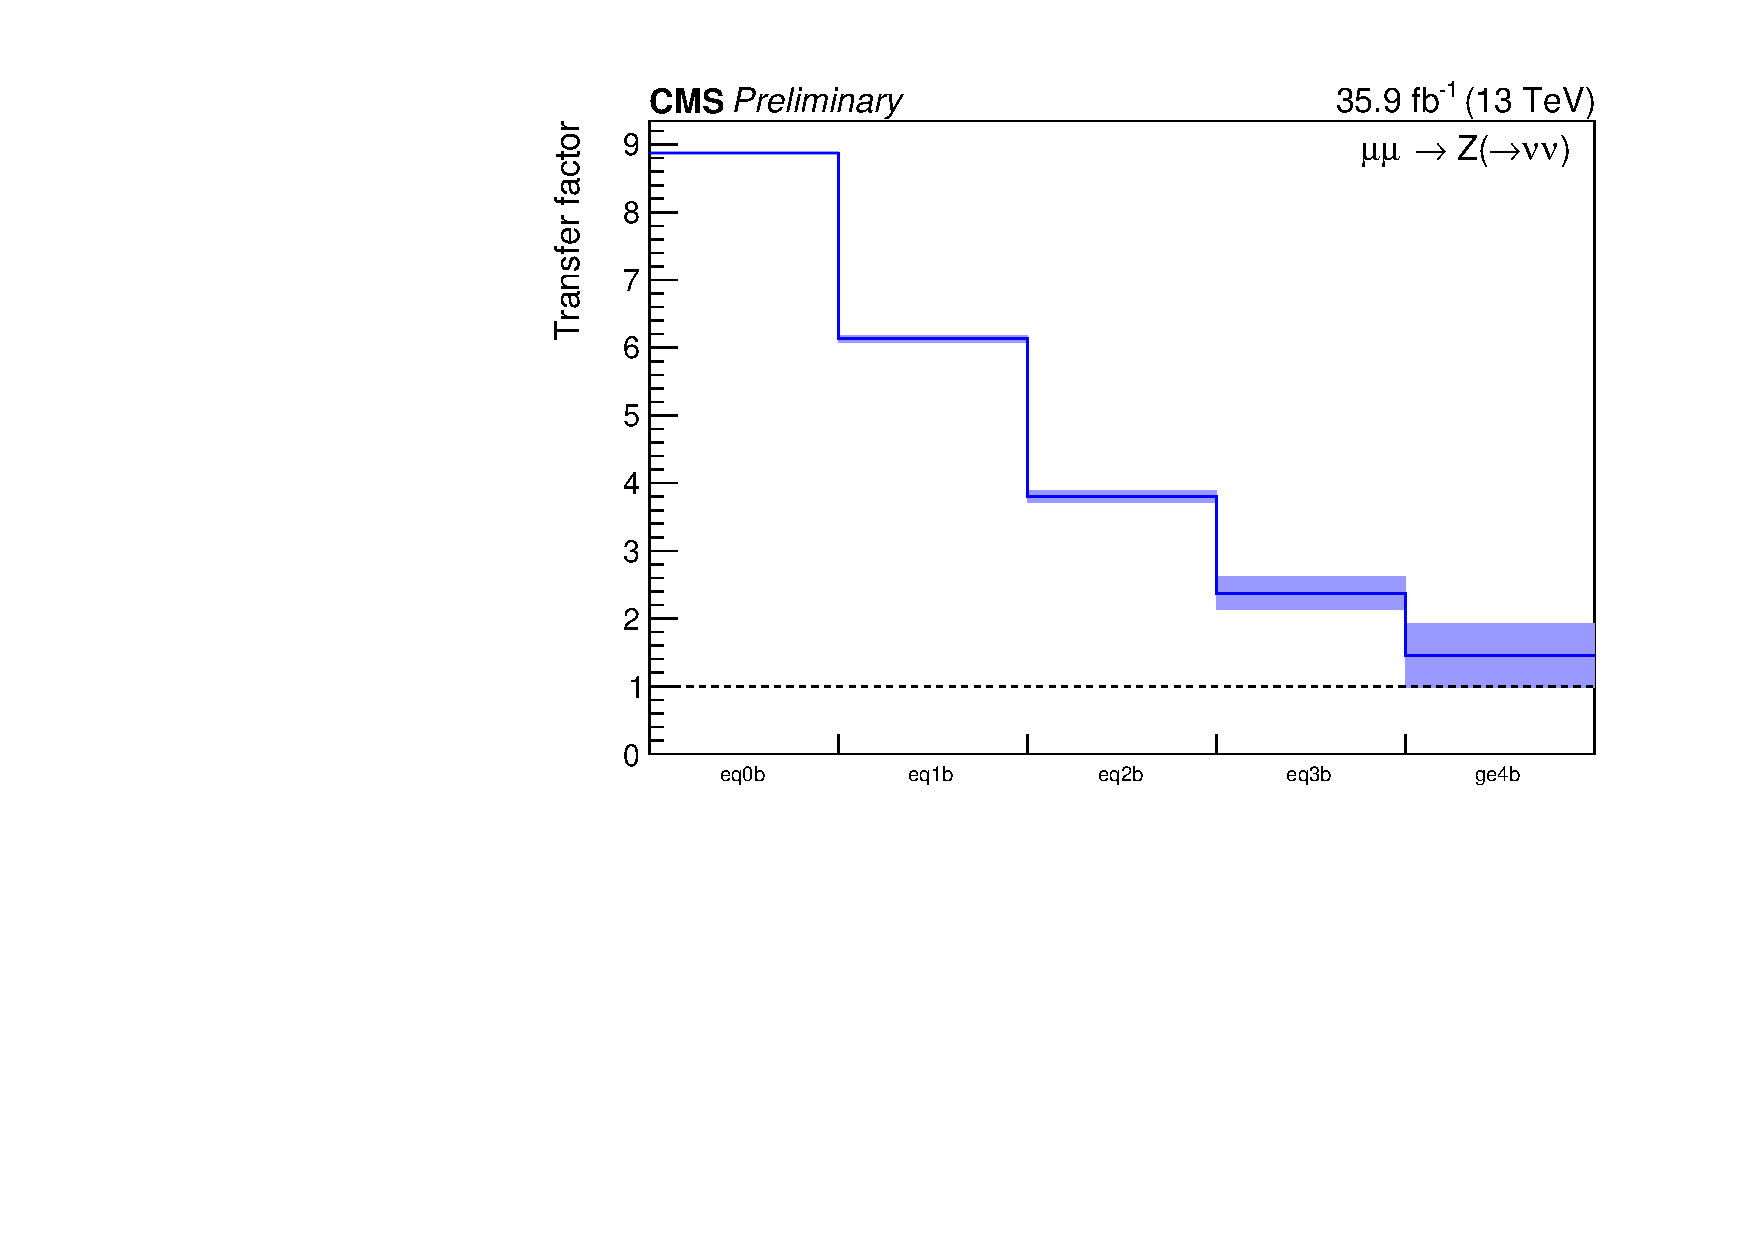
\includegraphics[width=0.5\textwidth]{figures/mcSystematics36p4fb/plots/tf_mumu_Zinv_bjet_nominalUp.pdf}
  } ~
  \subfigure[Transfer factor as a function of \mht.]{
    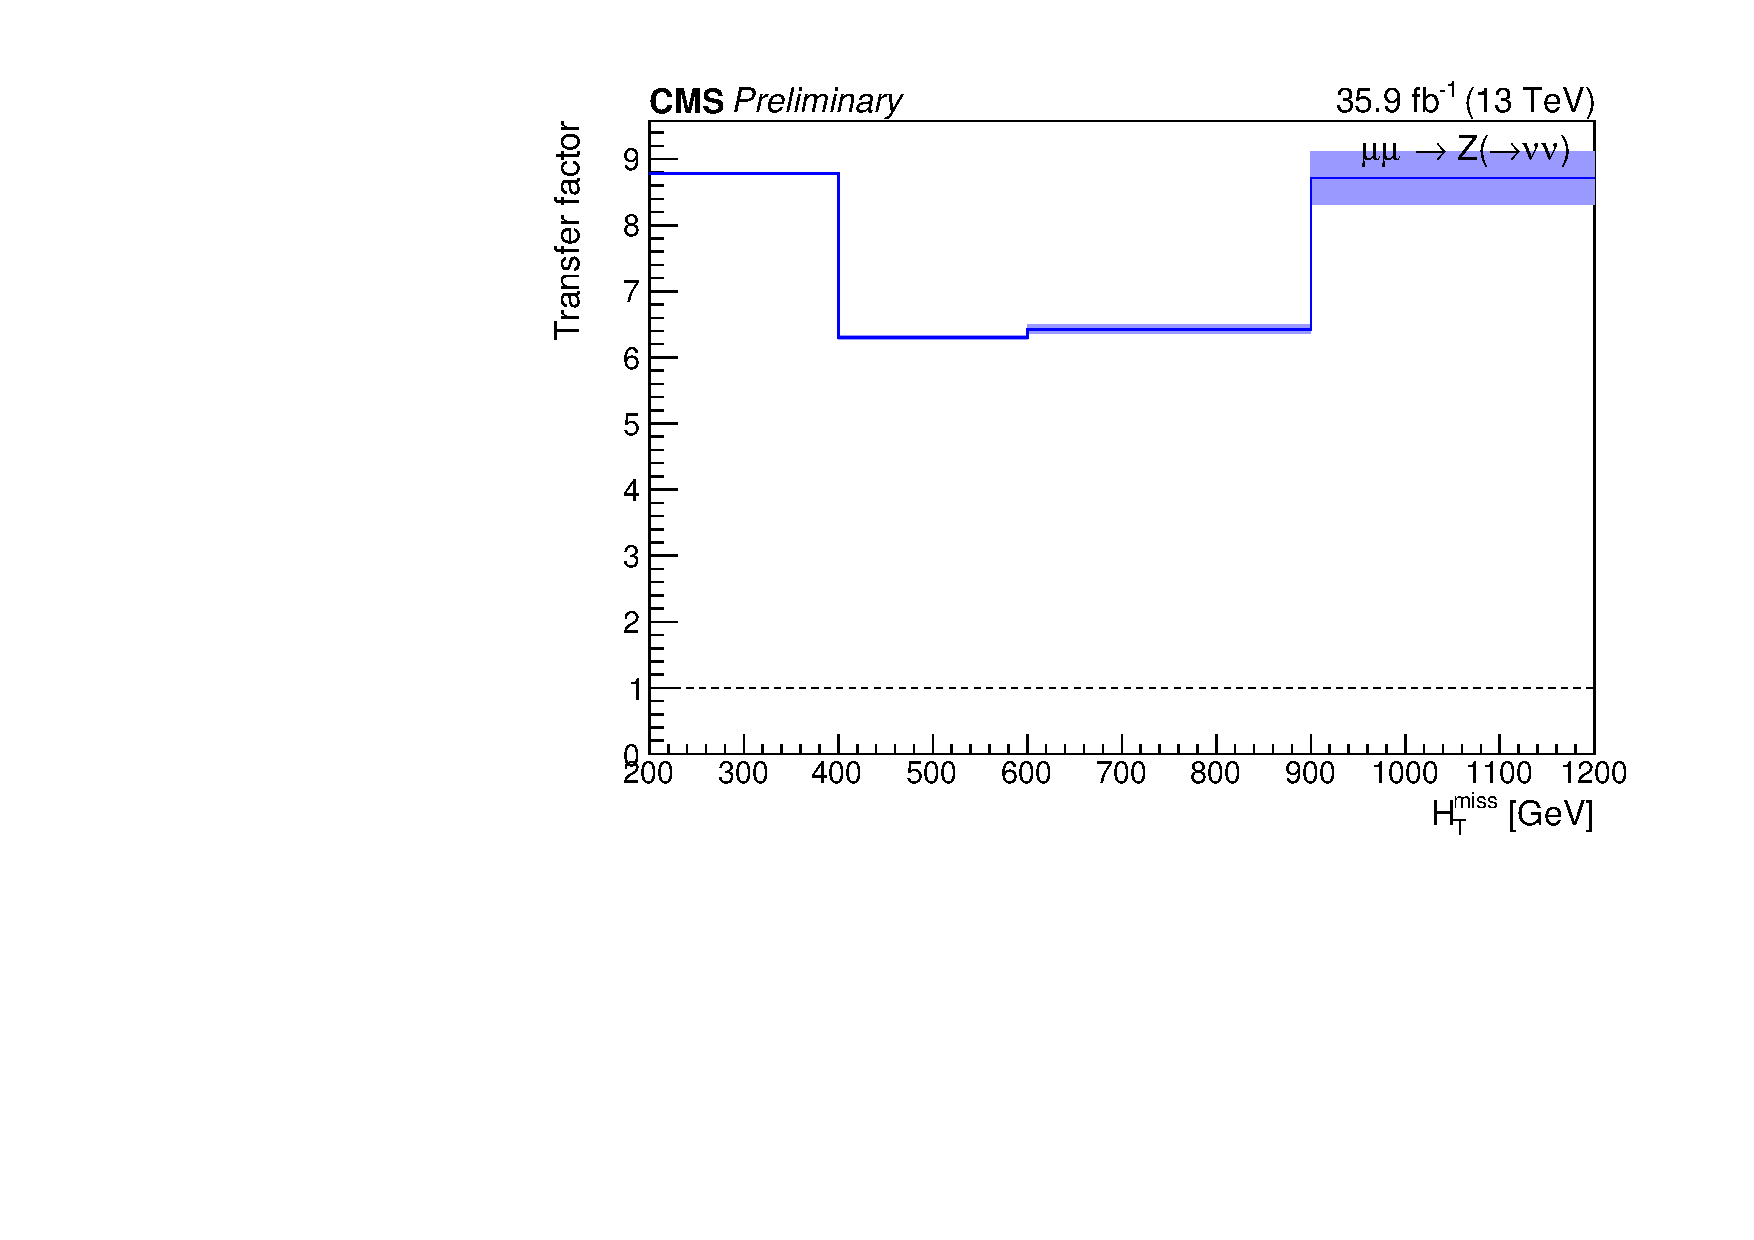
\includegraphics[width=0.5\textwidth]{figures/mcSystematics36p4fb/plots/tf_mumu_Zinv_mht_nominalUp.pdf}
  } \\
  \caption{\label{fig:tf_mmZinv} Transfer factors as a function of
    (\njet, \nb) event category and \scalht. Also shown are
    ``inclusive'' transfer factors as a function of \njet, \scalht,
    \nb, and \HTmiss. (Each ``inclusive'' dependence is shown when
    integrating over all other variables.) }
\end{figure}

\clearpage
\subsection{Minimum bias cross section / pileup}

\begin{figure}[!h]
  \centering
  \subfigure[Up variation versus (\njet,\nb) category and \scalht.]{
    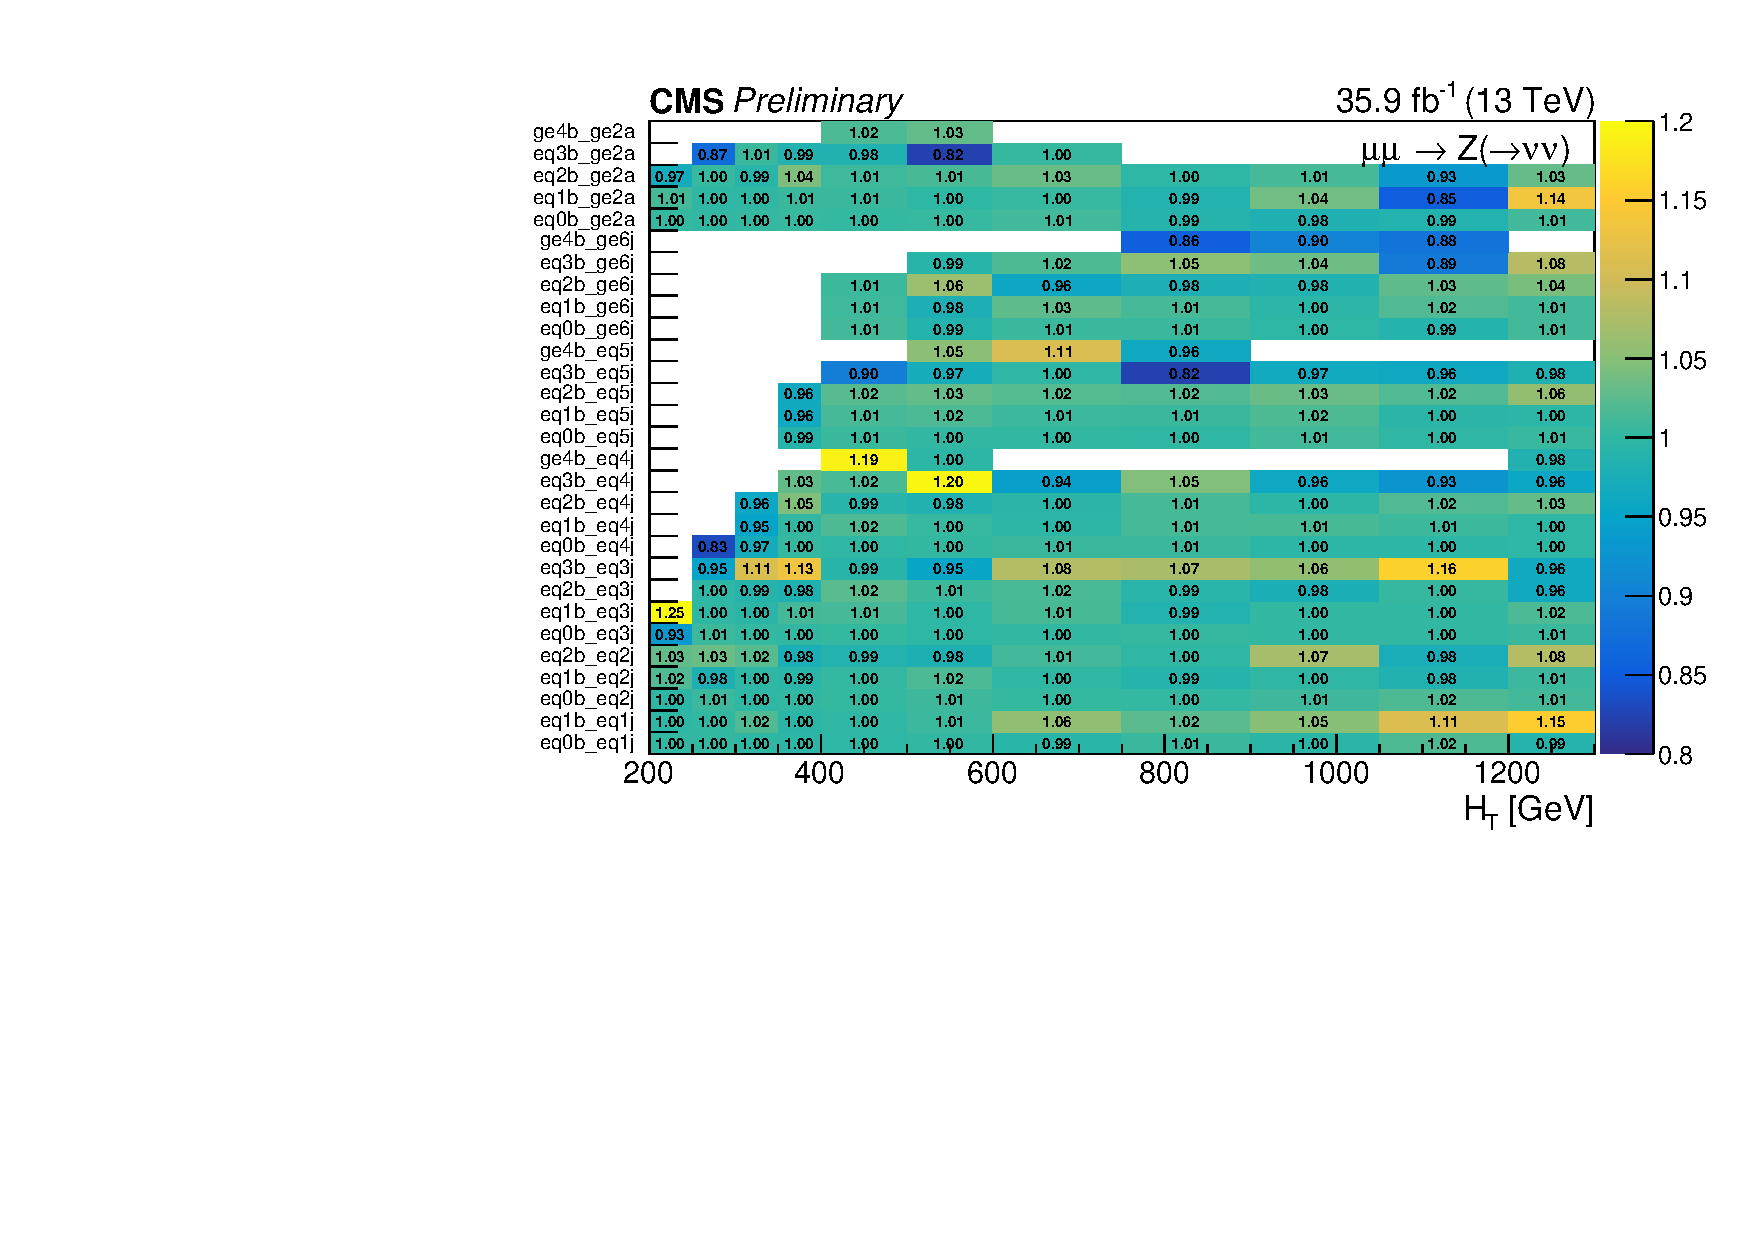
\includegraphics[width=0.5\textwidth]{figures/mcSystematics36p4fb/plots/tfratio_mumu_Zinv_2d_puWeightUp.pdf}
  } ~
  \subfigure[Down variation versus (\njet,\nb) category and \scalht.]{
    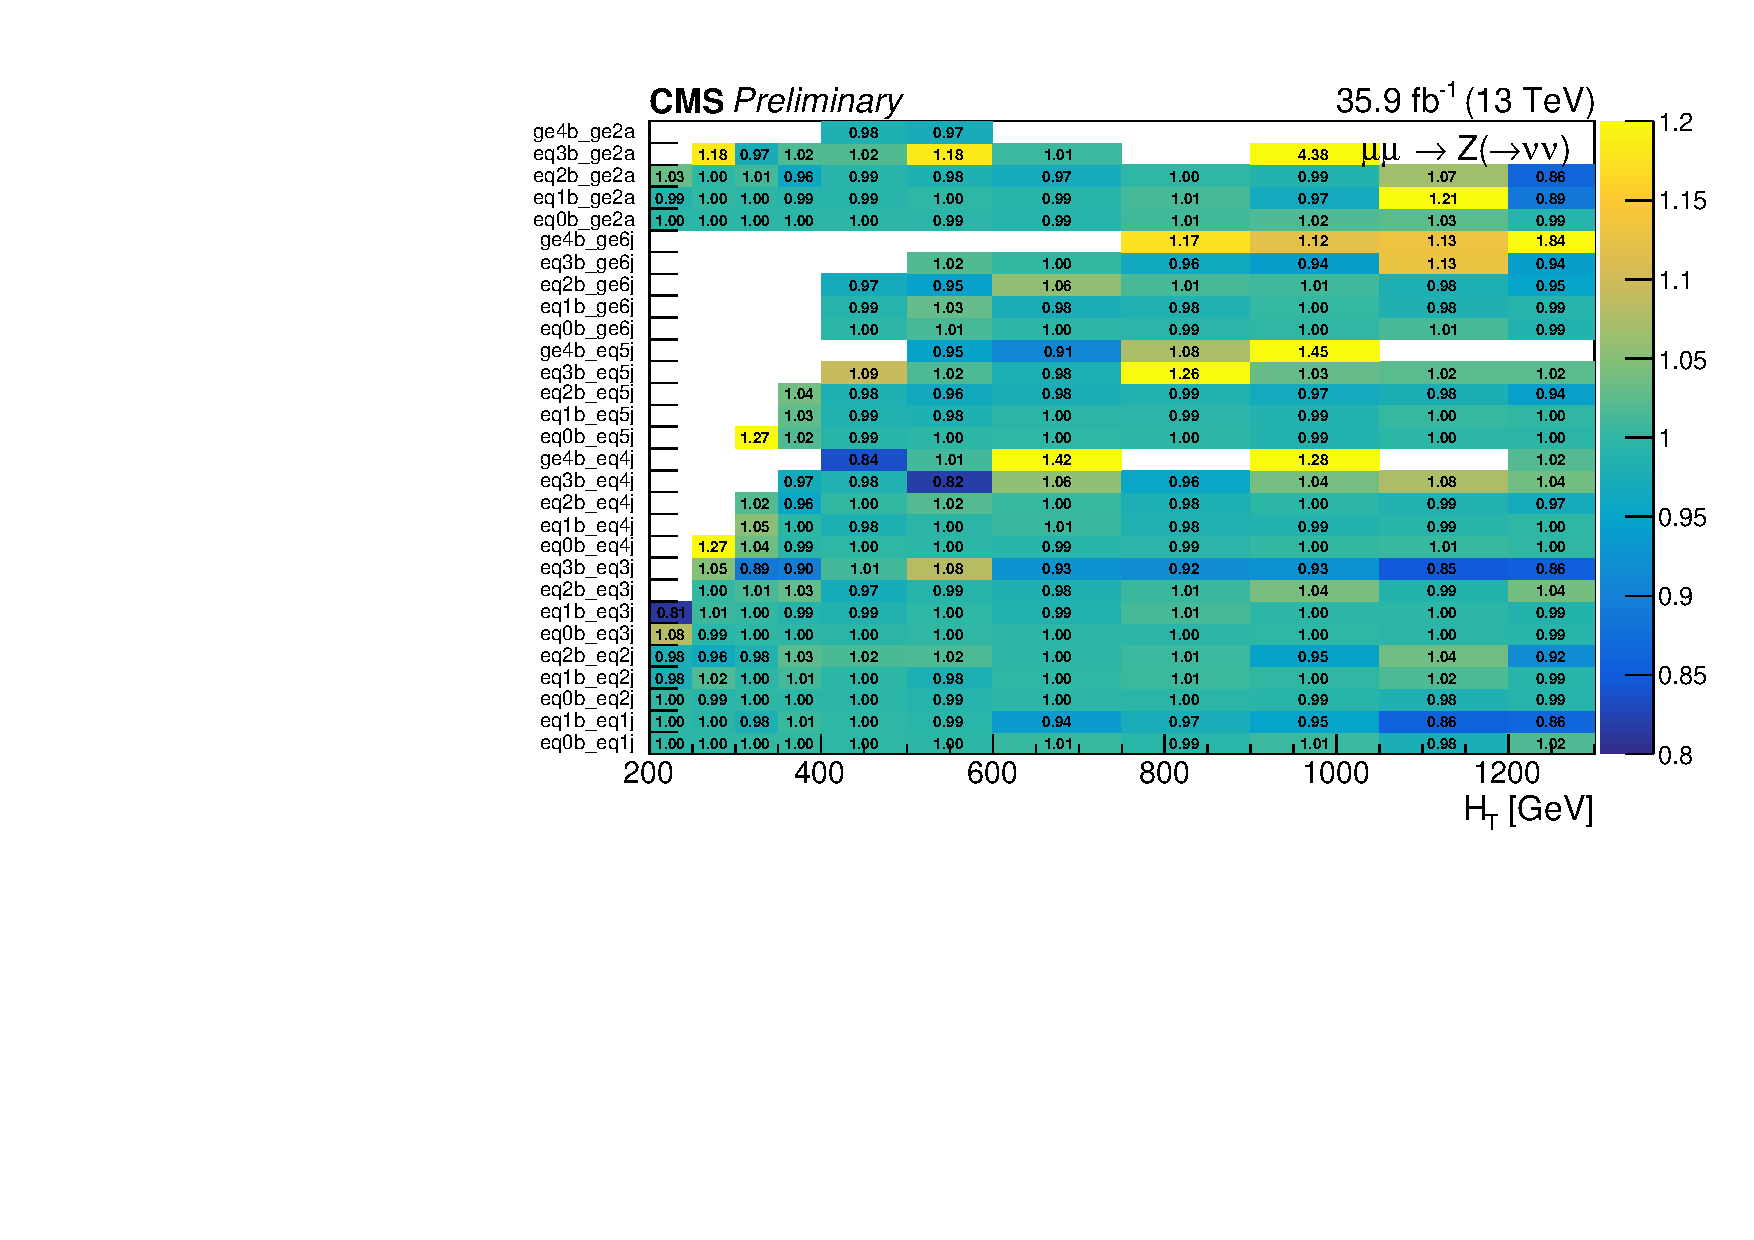
\includegraphics[width=0.5\textwidth]{figures/mcSystematics36p4fb/plots/tfratio_mumu_Zinv_2d_puWeightDown.pdf}
  }\\
  \subfigure[Up/down variations versus \njet.]{
    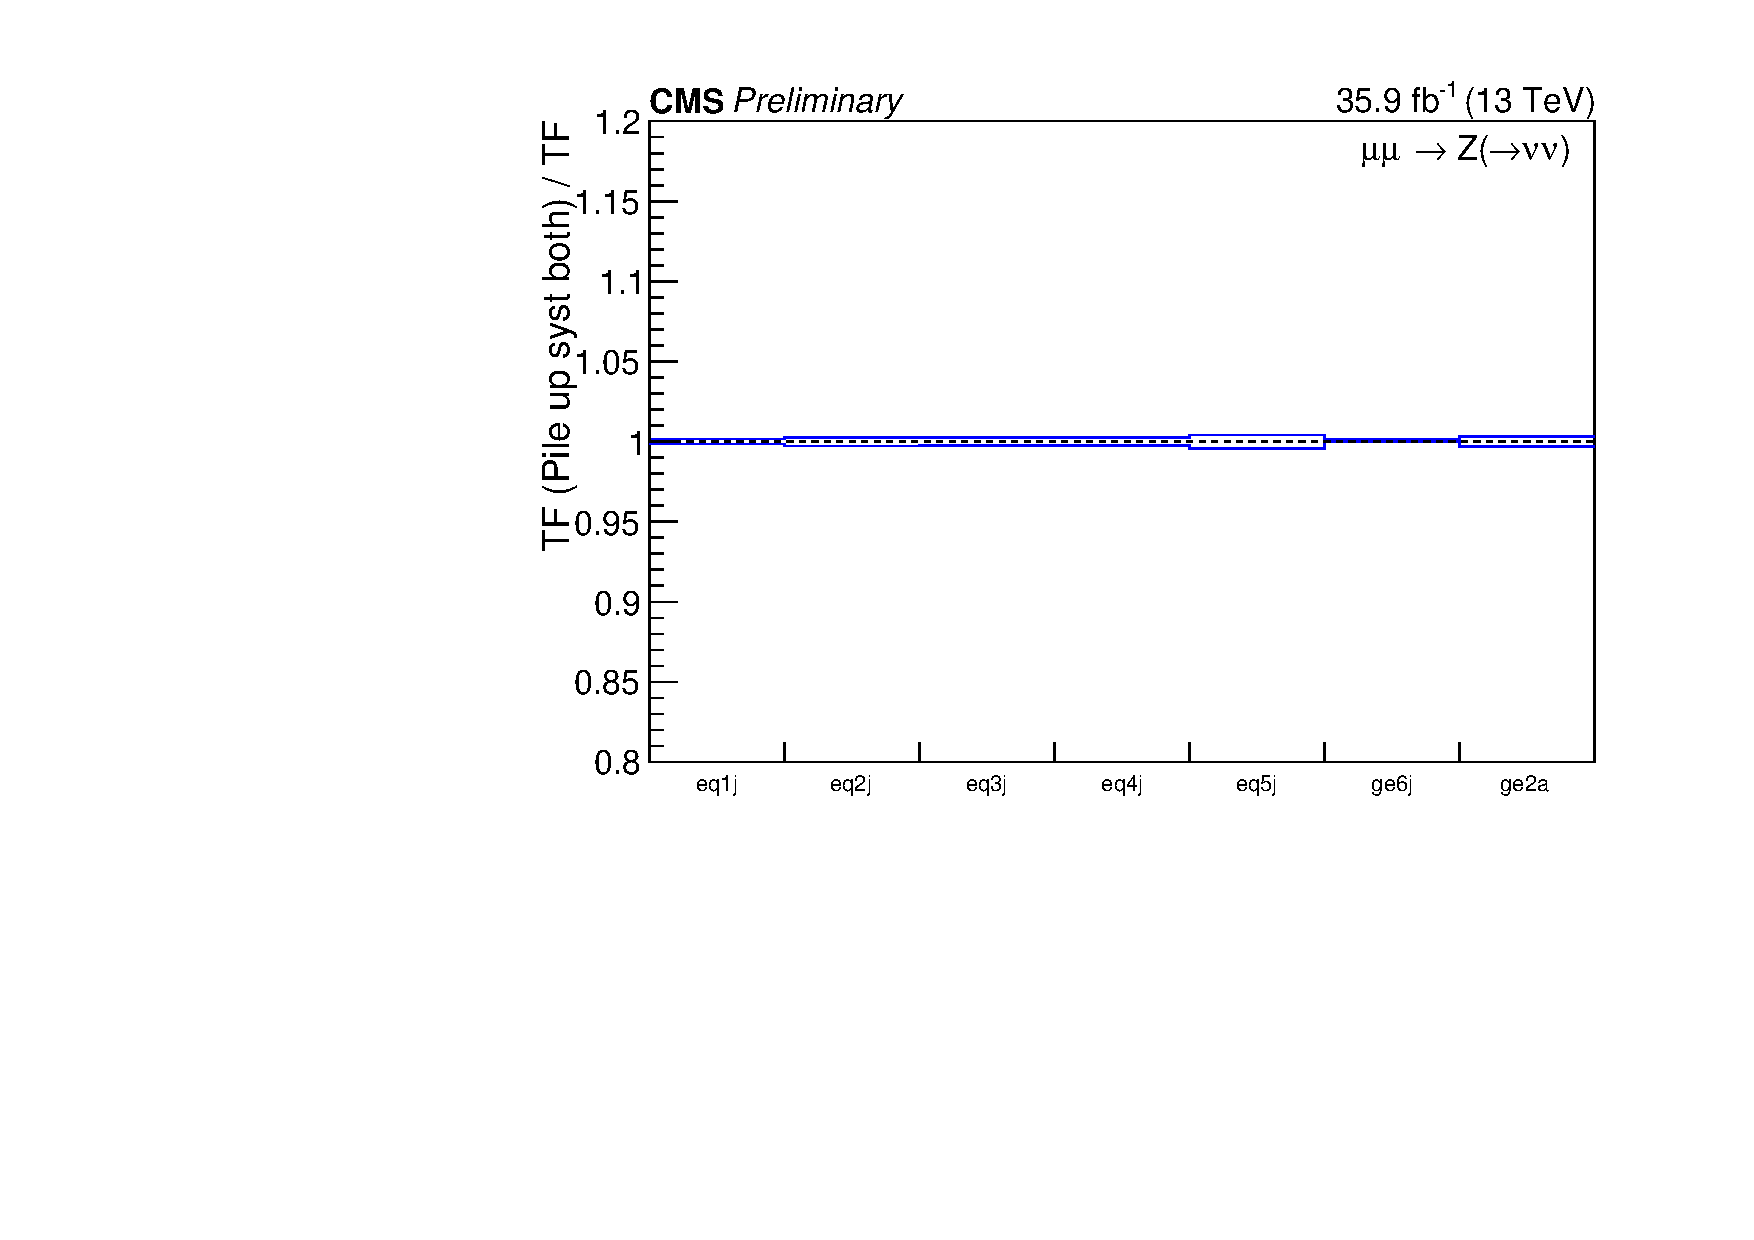
\includegraphics[width=0.5\textwidth]{figures/mcSystematics36p4fb/plots/tfratio_mumu_Zinv_njet_puWeightUp.pdf}
  } ~
  \subfigure[Up/down variations versus \scalht.]{
    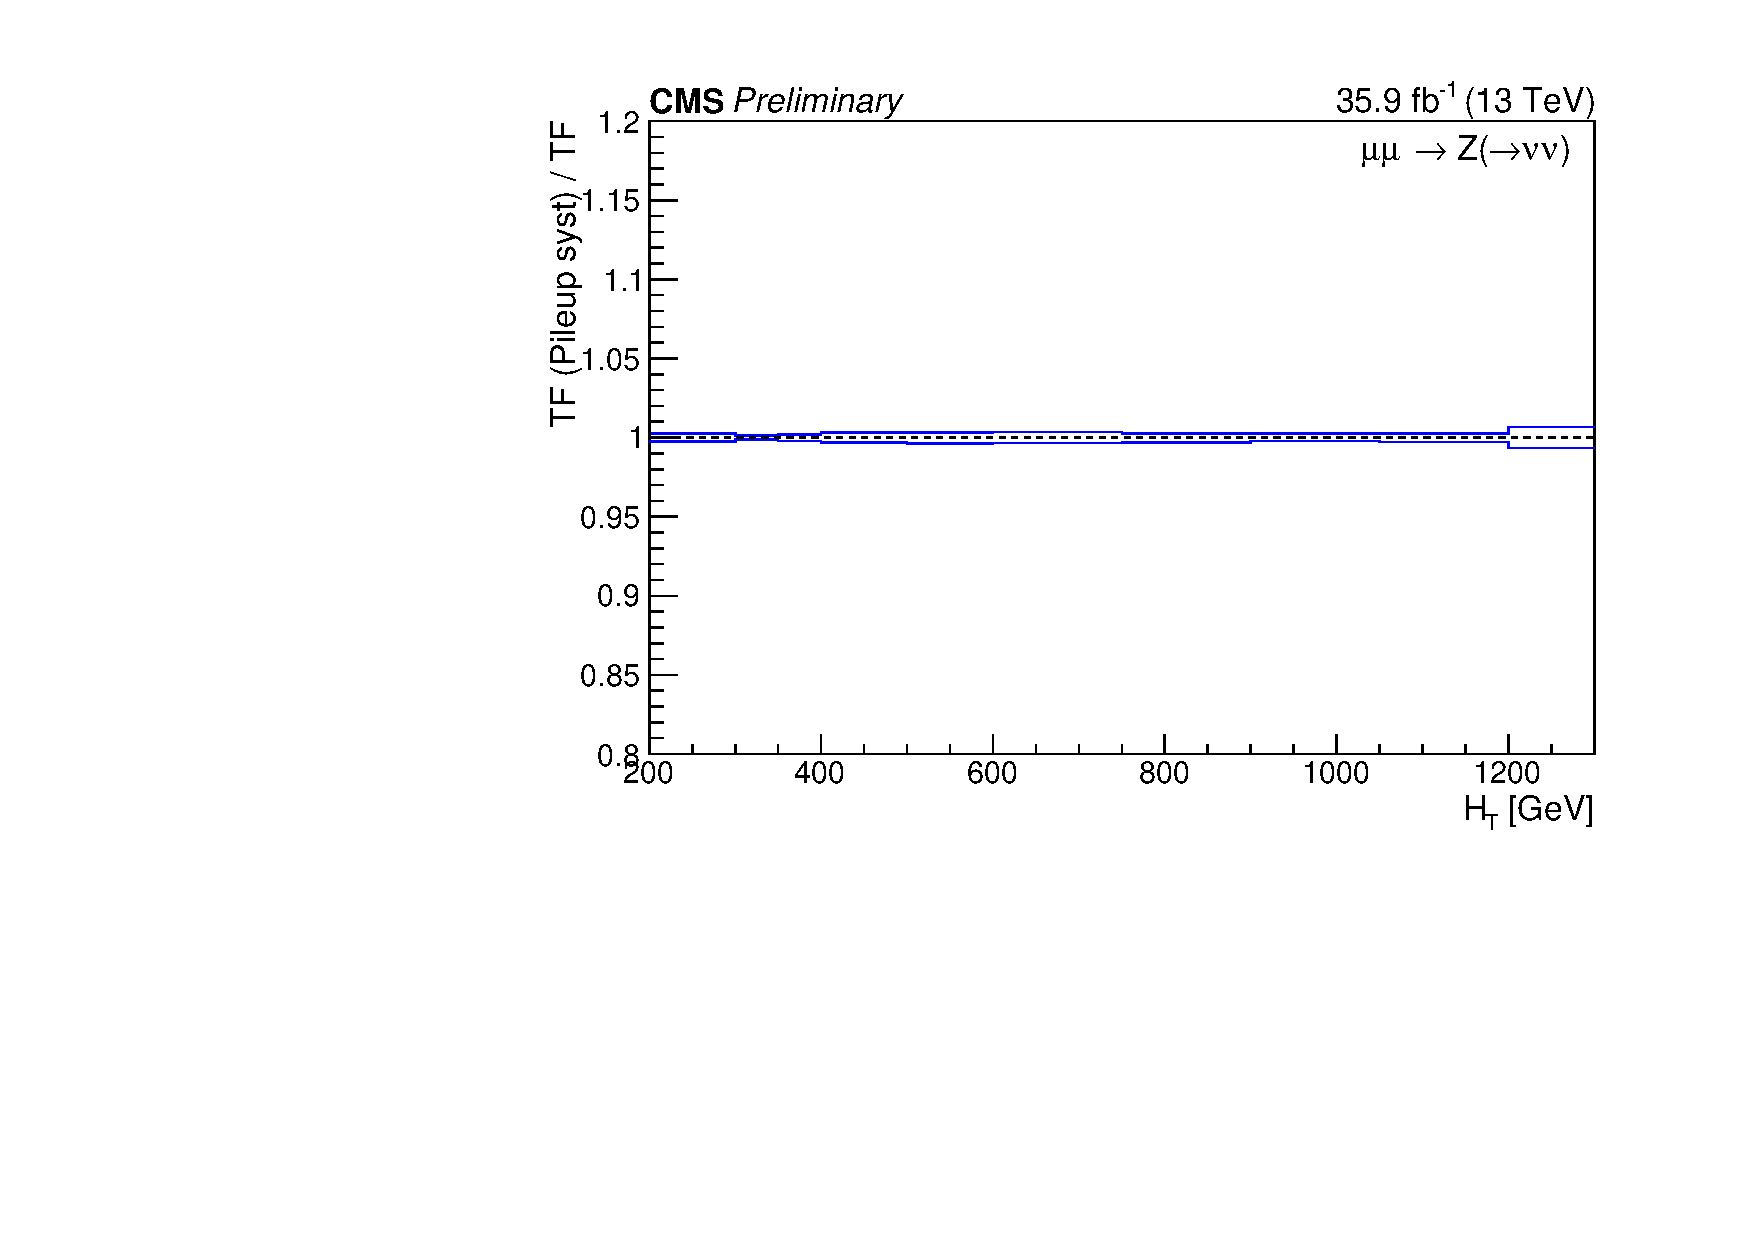
\includegraphics[width=0.5\textwidth]{figures/mcSystematics36p4fb/plots/tfratio_mumu_Zinv_ht_puWeightUp.pdf}
  } \\
  \subfigure[Up/down variations versus \nb.]{
    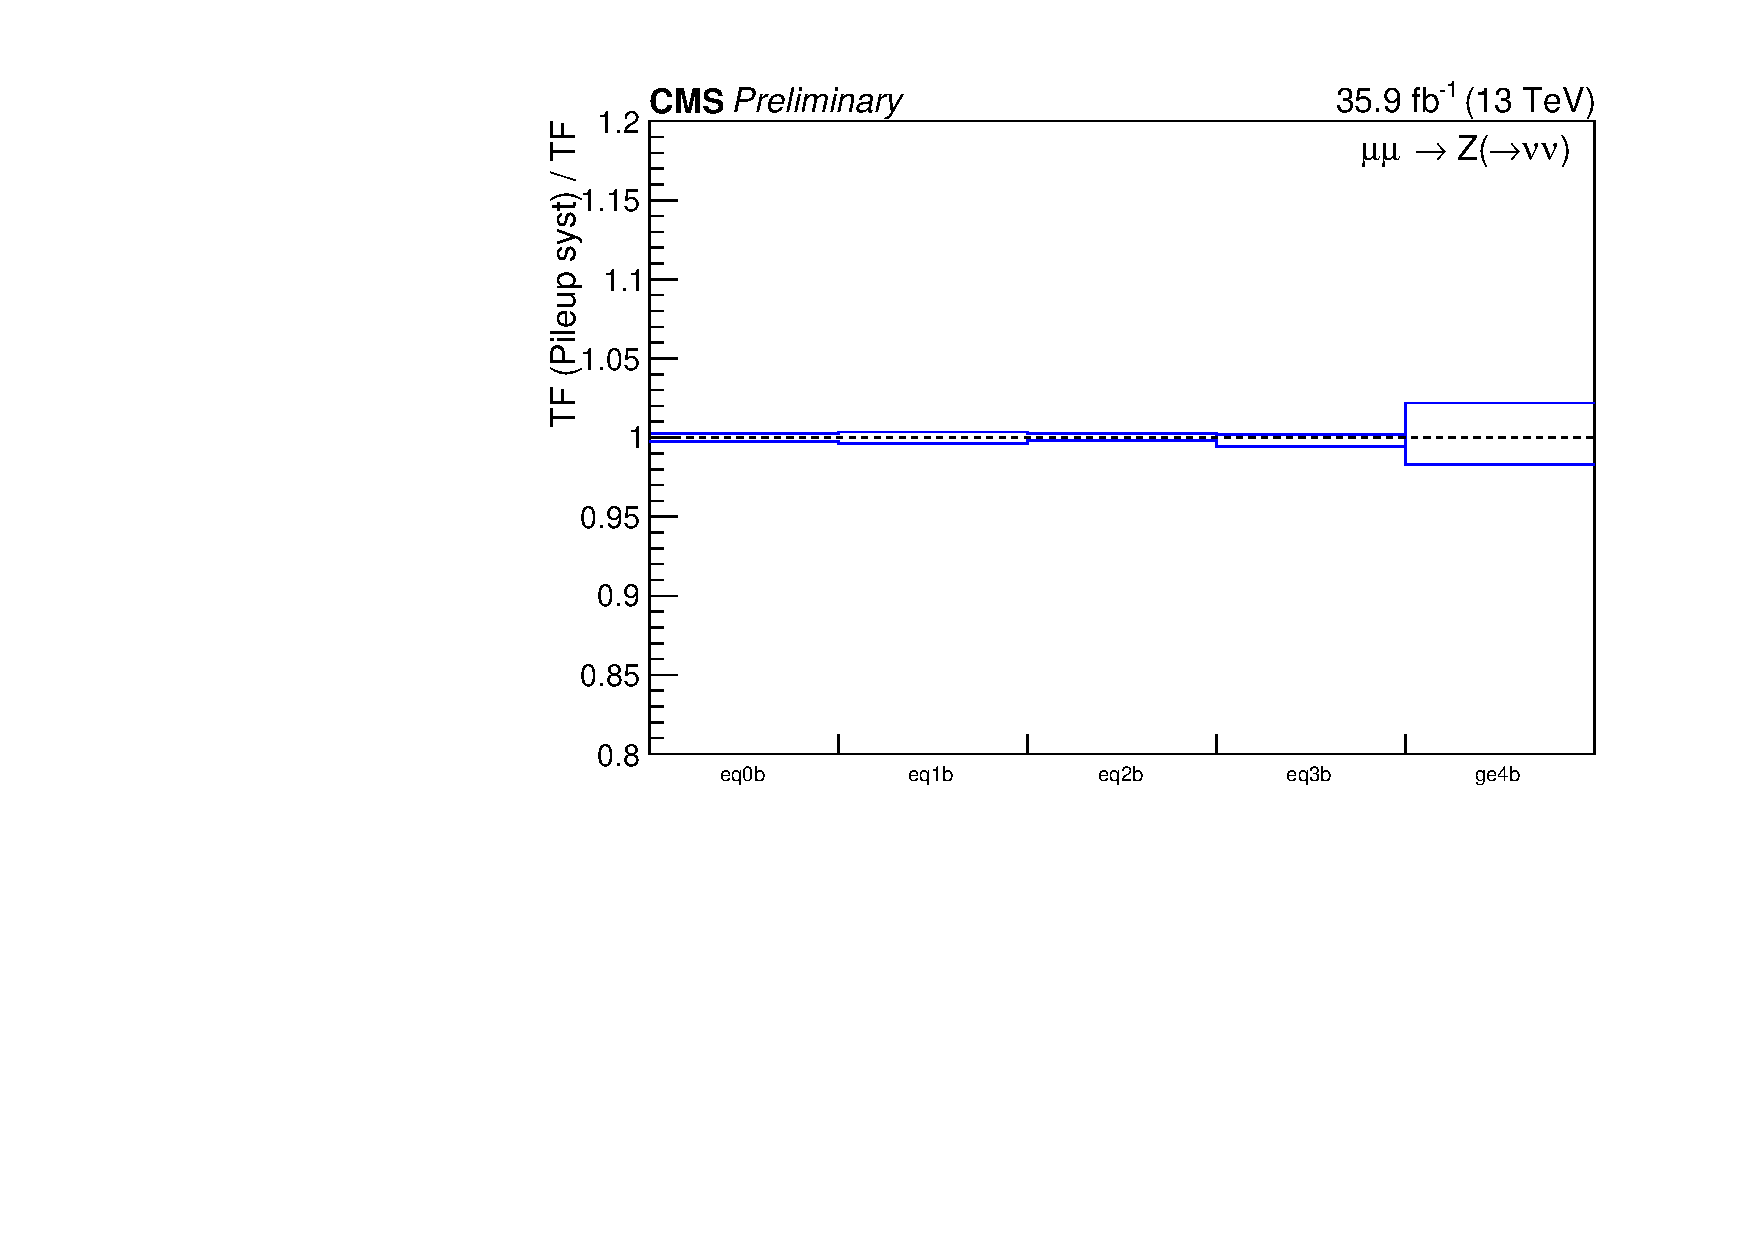
\includegraphics[width=0.5\textwidth]{figures/mcSystematics36p4fb/plots/tfratio_mumu_Zinv_bjet_puWeightUp.pdf}
  } ~
  \subfigure[Up/down variations versus \mht.]{
    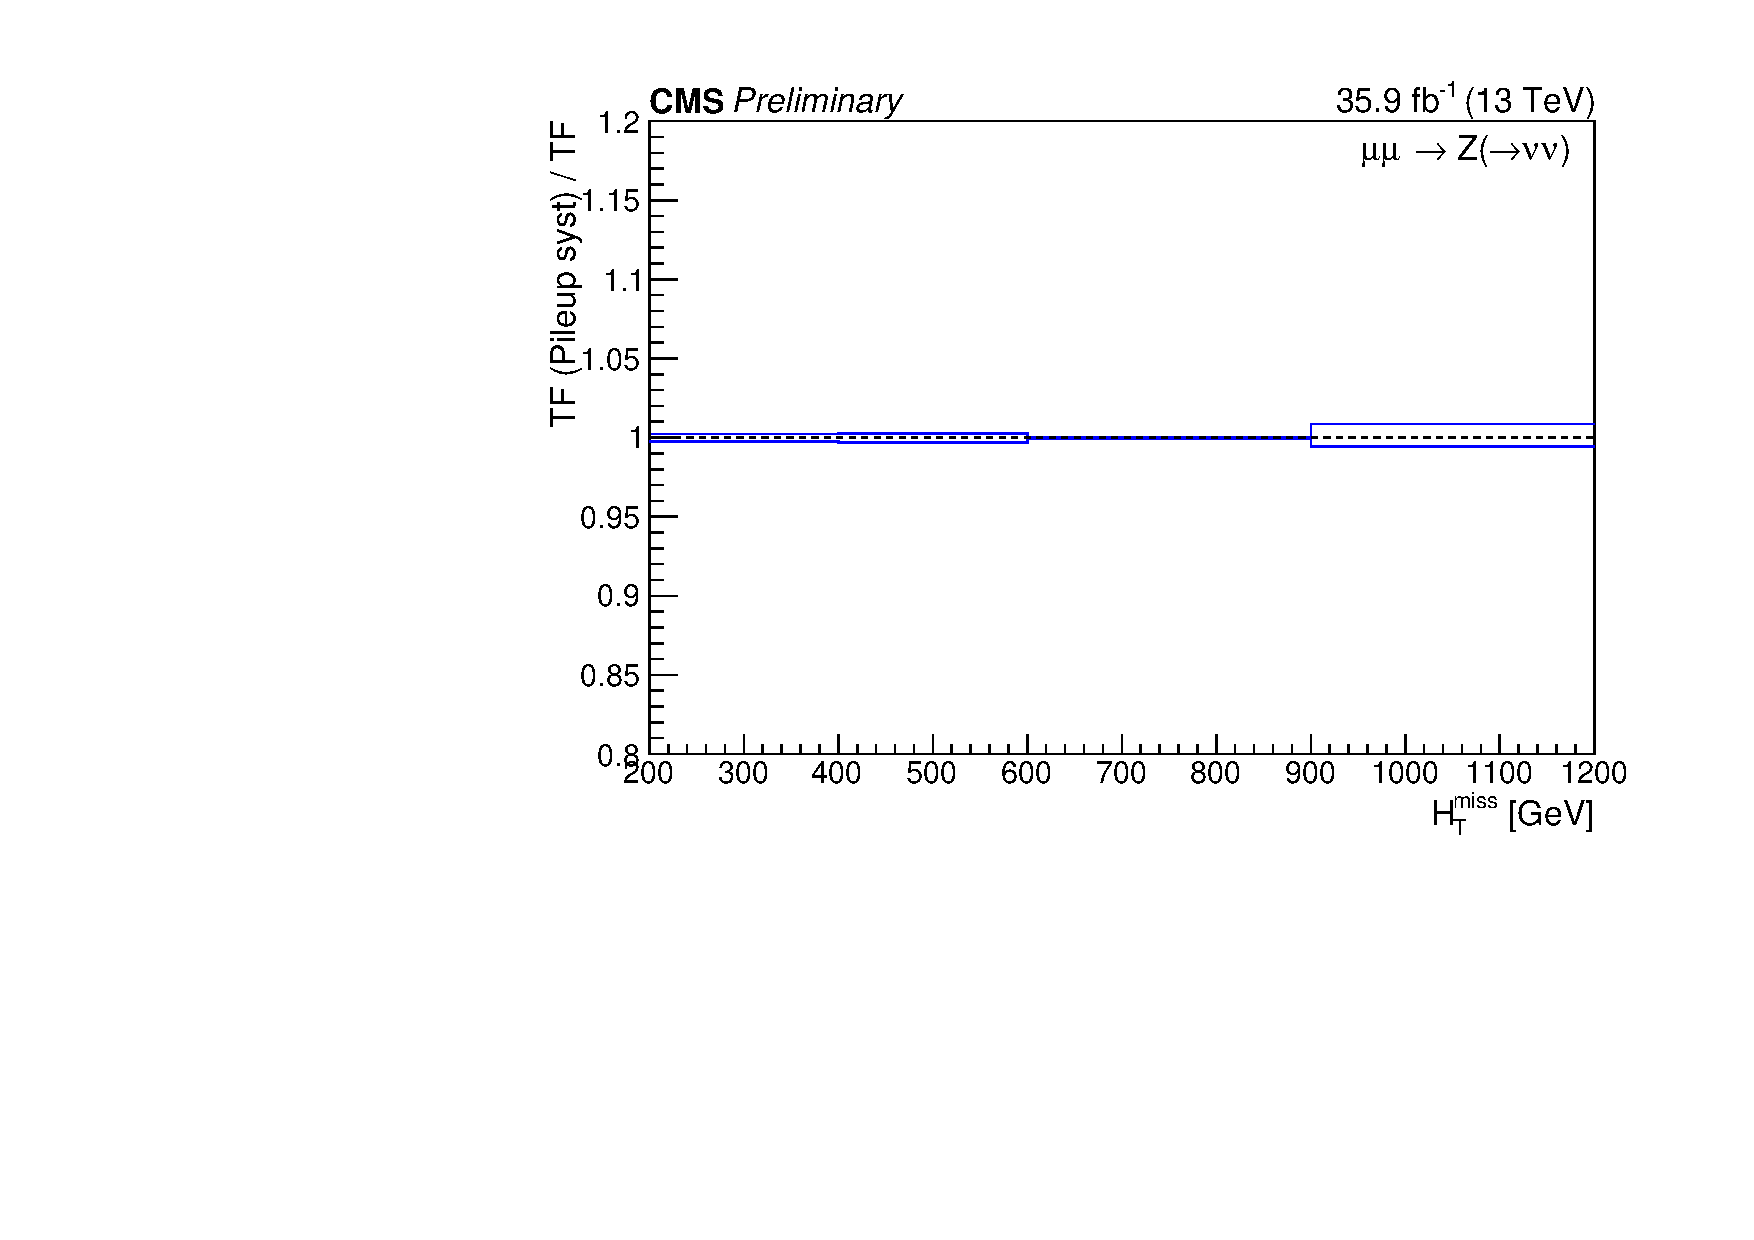
\includegraphics[width=0.5\textwidth]{figures/mcSystematics36p4fb/plots/tfratio_mumu_Zinv_mht_puWeightUp.pdf}
  } \\
  \caption{\label{fig:tfSyst_pu_mmZinv} The relative change in the
    ``$\mmj \rightarrow \znunu\ + \textrm{jets}$'' transfer factors from
    simulation due to $\pm1\sigma$ uncertainties in pileup.  }
\end{figure}

\clearpage
\subsection{Effect of scale and PDF on lepton acceptance}

\begin{figure}[!h]
  \centering
  \subfigure[Up variation versus (\njet,\nb) category and \scalht.]{
    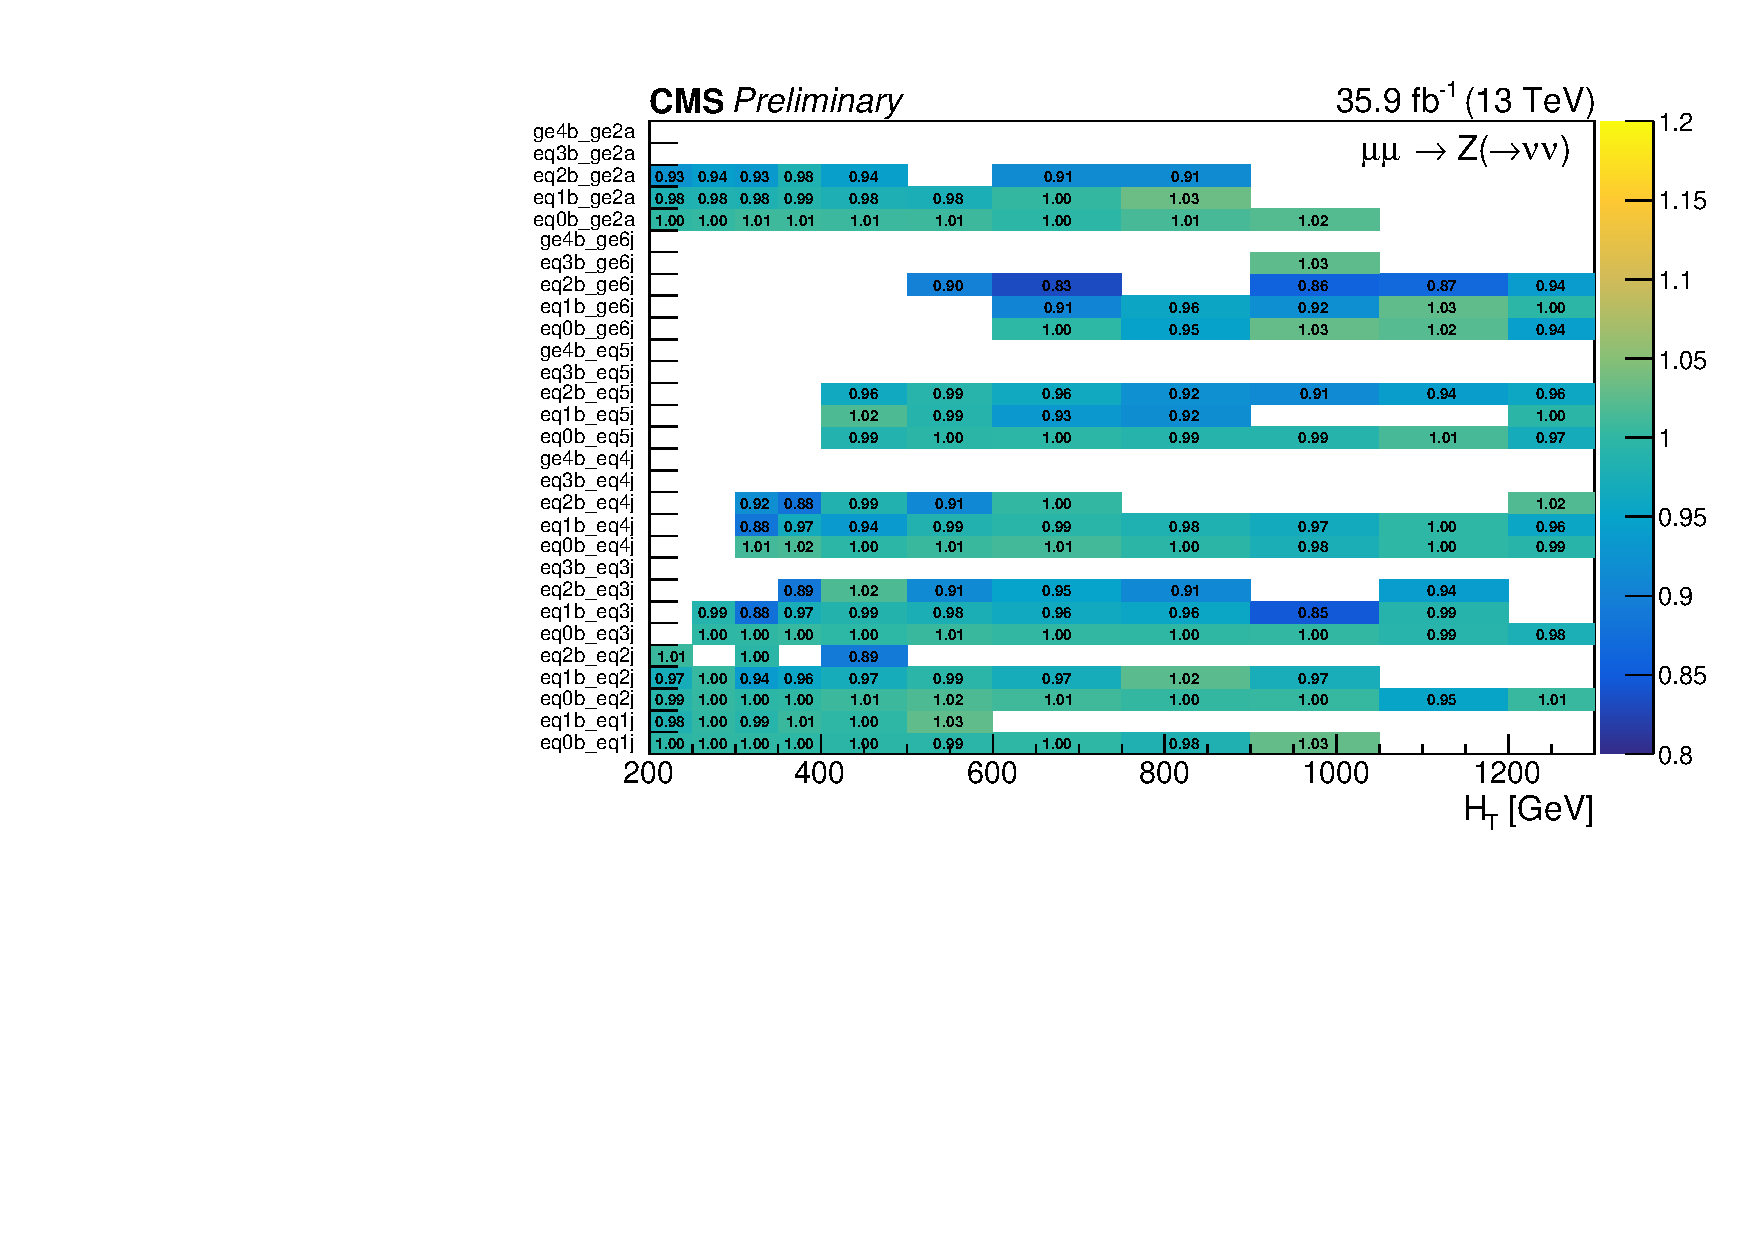
\includegraphics[width=0.5\textwidth]{figures/mcSystematics36p4fb/plots/tfratio_mumu_Zinv_2d_scaleWeightUp.pdf}
  } ~
  \subfigure[Down variation versus (\njet,\nb) category and \scalht.]{
    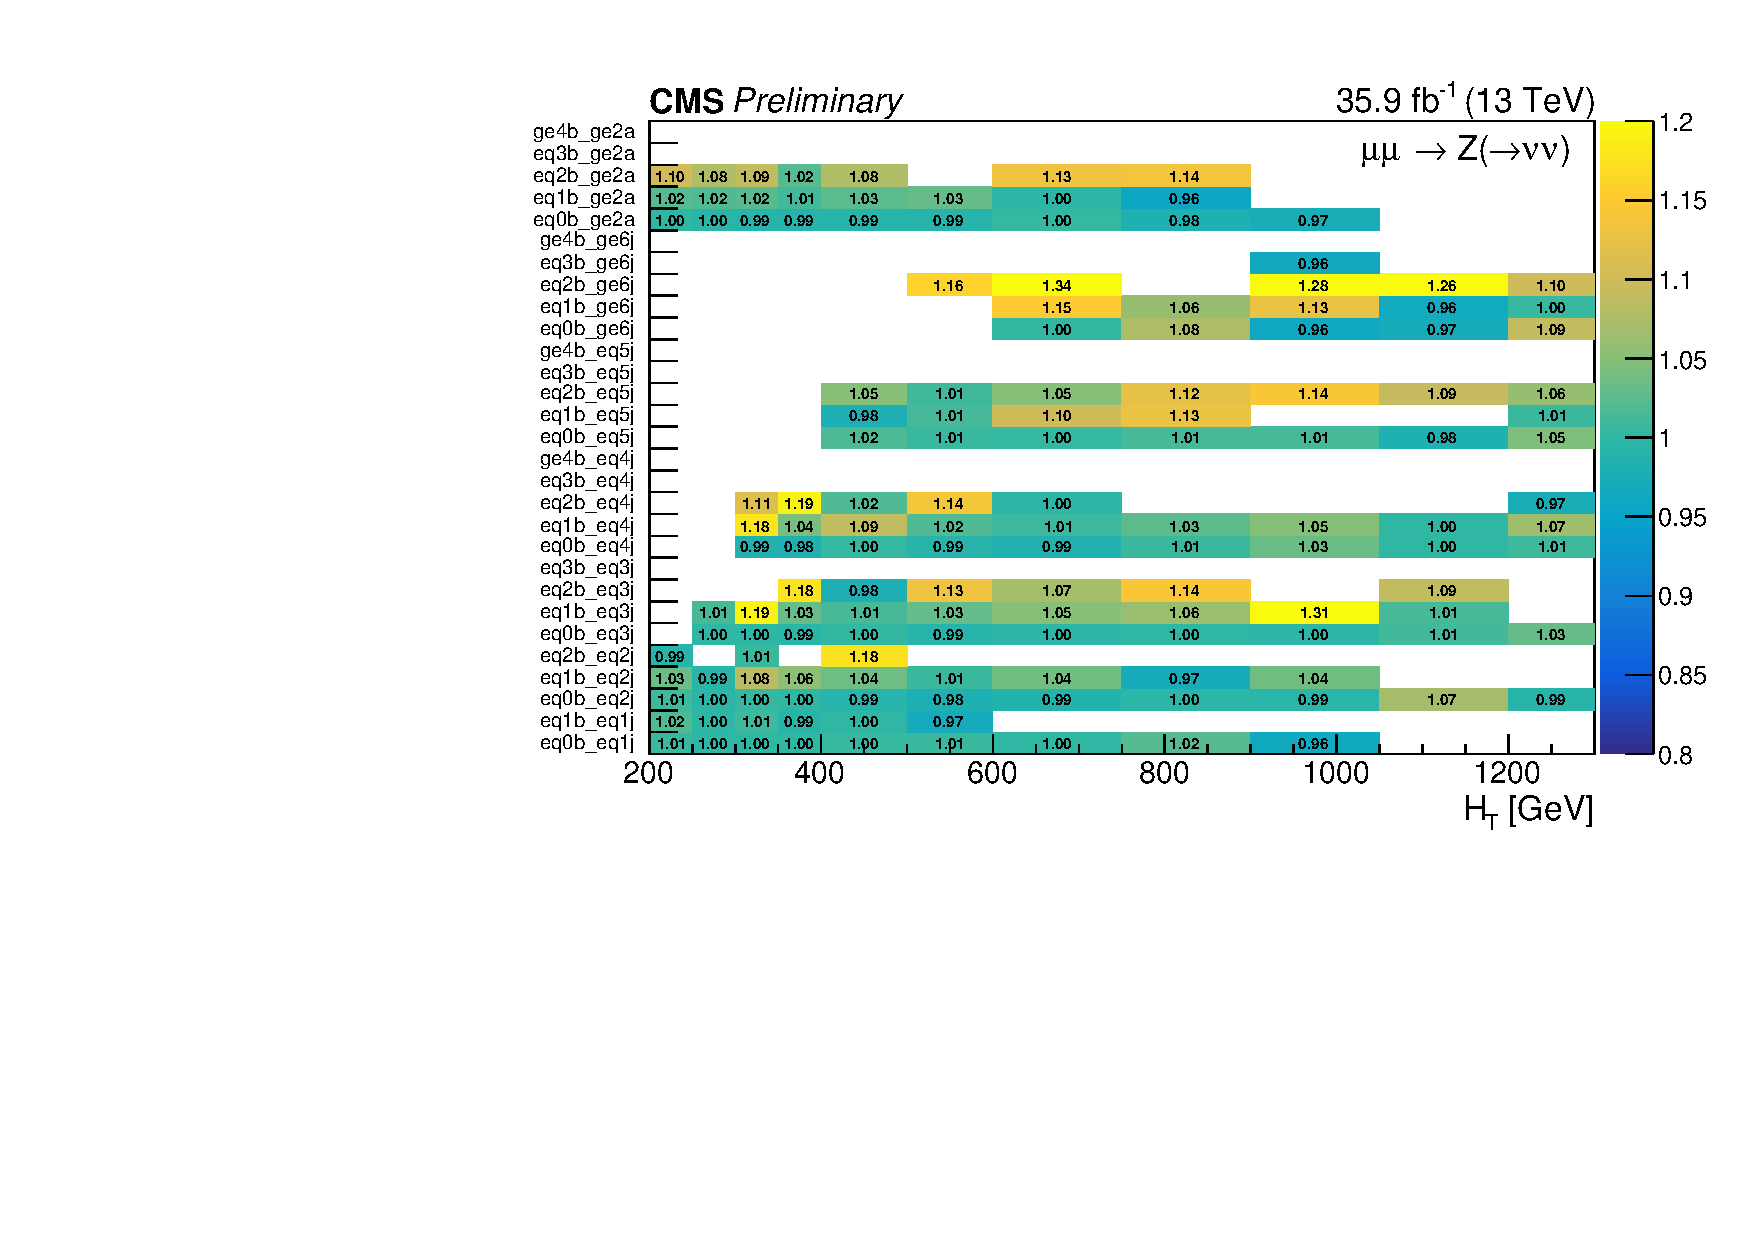
\includegraphics[width=0.5\textwidth]{figures/mcSystematics36p4fb/plots/tfratio_mumu_Zinv_2d_scaleWeightDown.pdf}
  }\\
  \subfigure[Up/down variations versus \njet.]{
    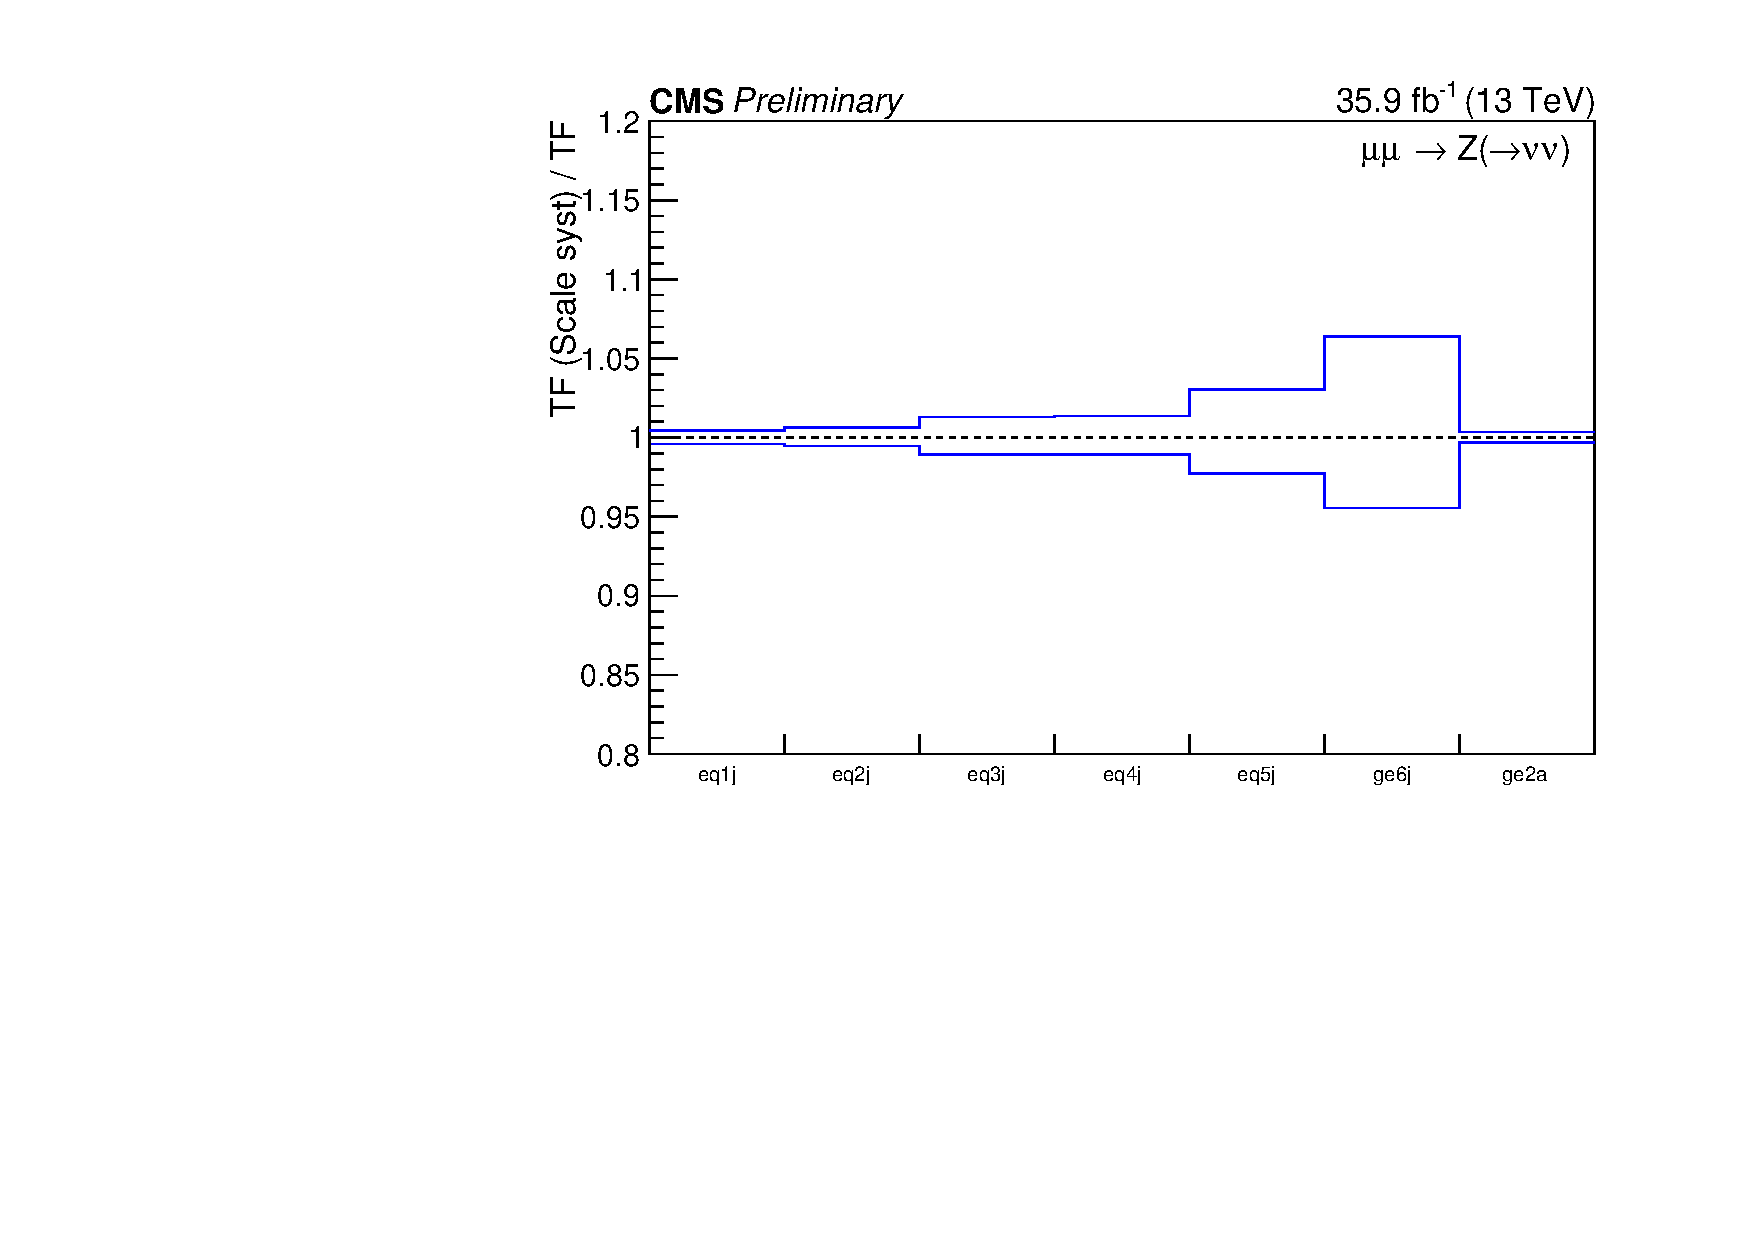
\includegraphics[width=0.5\textwidth]{figures/mcSystematics36p4fb/plots/tfratio_mumu_Zinv_njet_scaleWeightUp.pdf}
  } ~
  \subfigure[Up/down variations versus \scalht.]{
    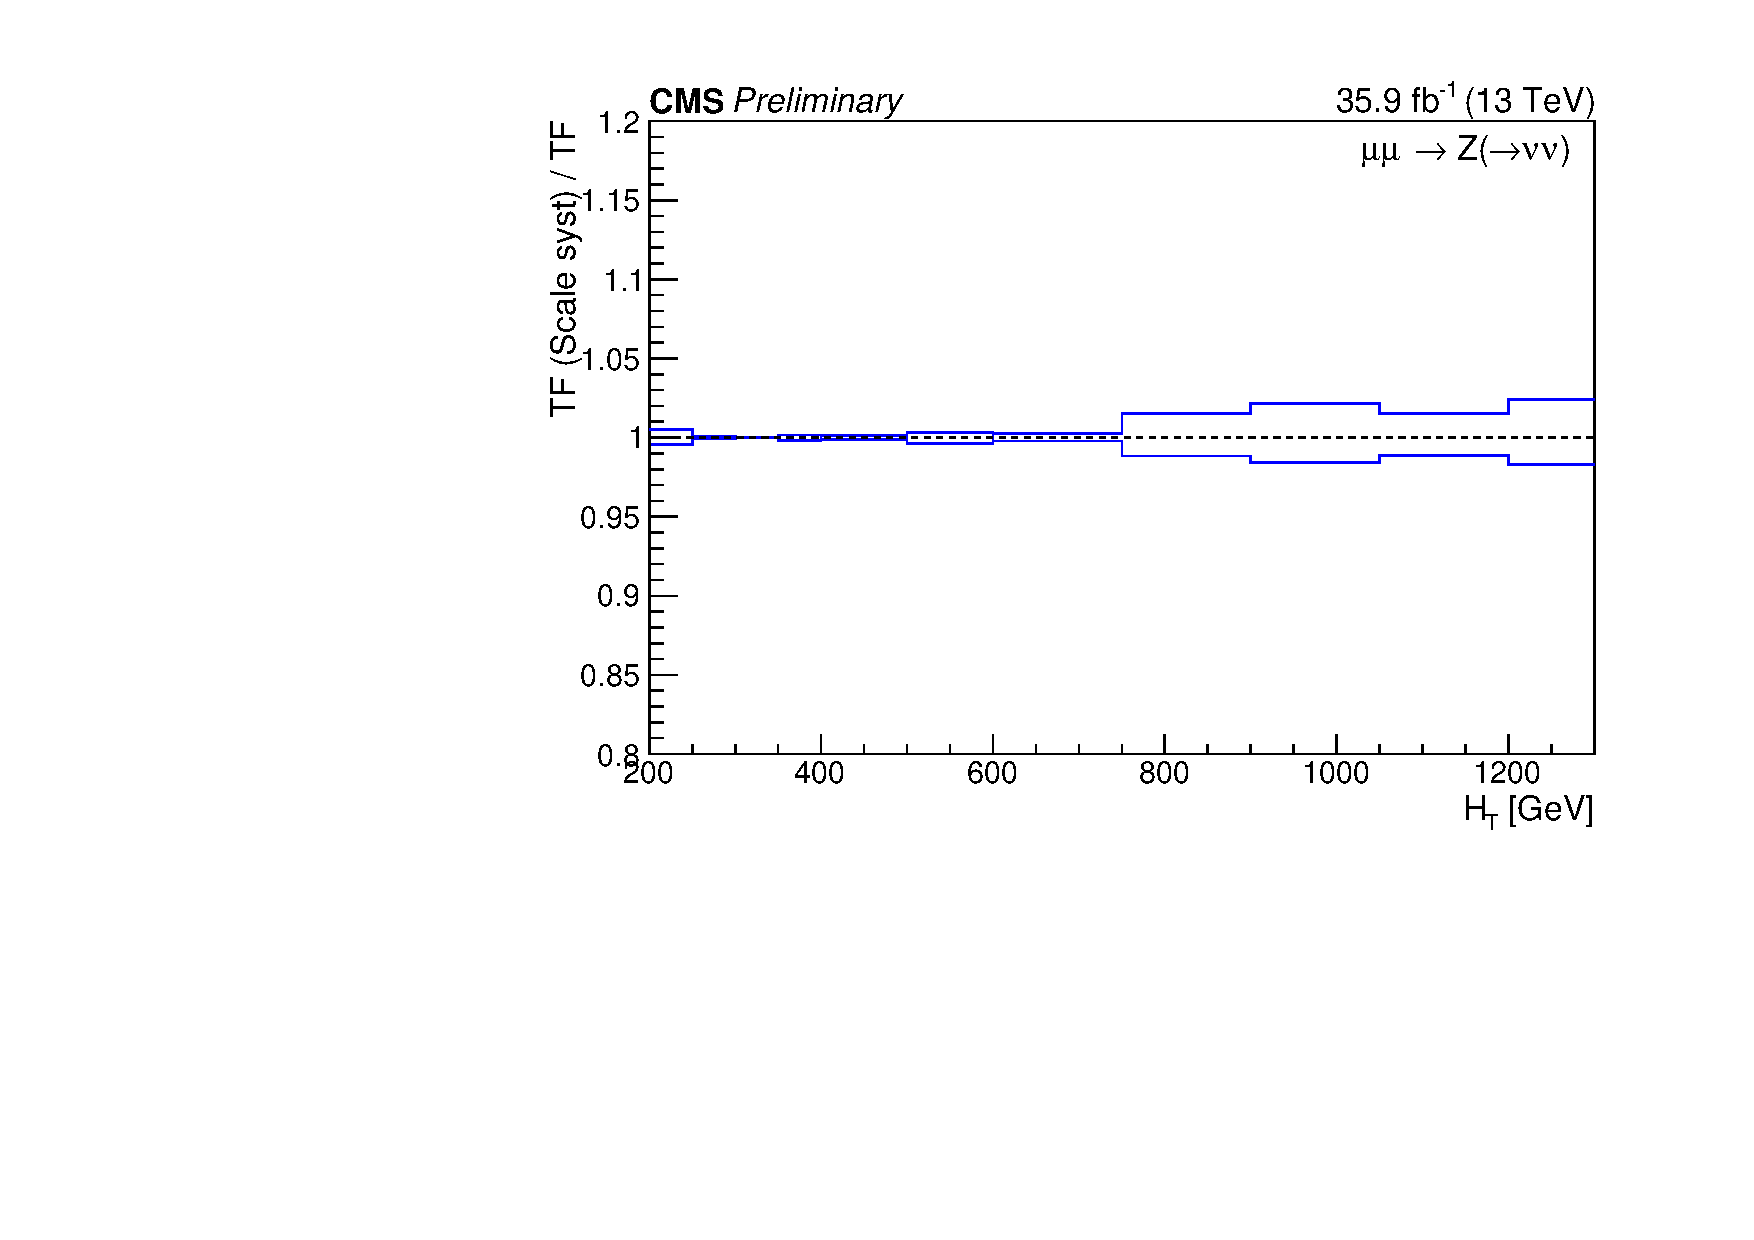
\includegraphics[width=0.5\textwidth]{figures/mcSystematics36p4fb/plots/tfratio_mumu_Zinv_ht_scaleWeightUp.pdf}
  } \\
  \subfigure[Up/down variations versus \nb.]{
    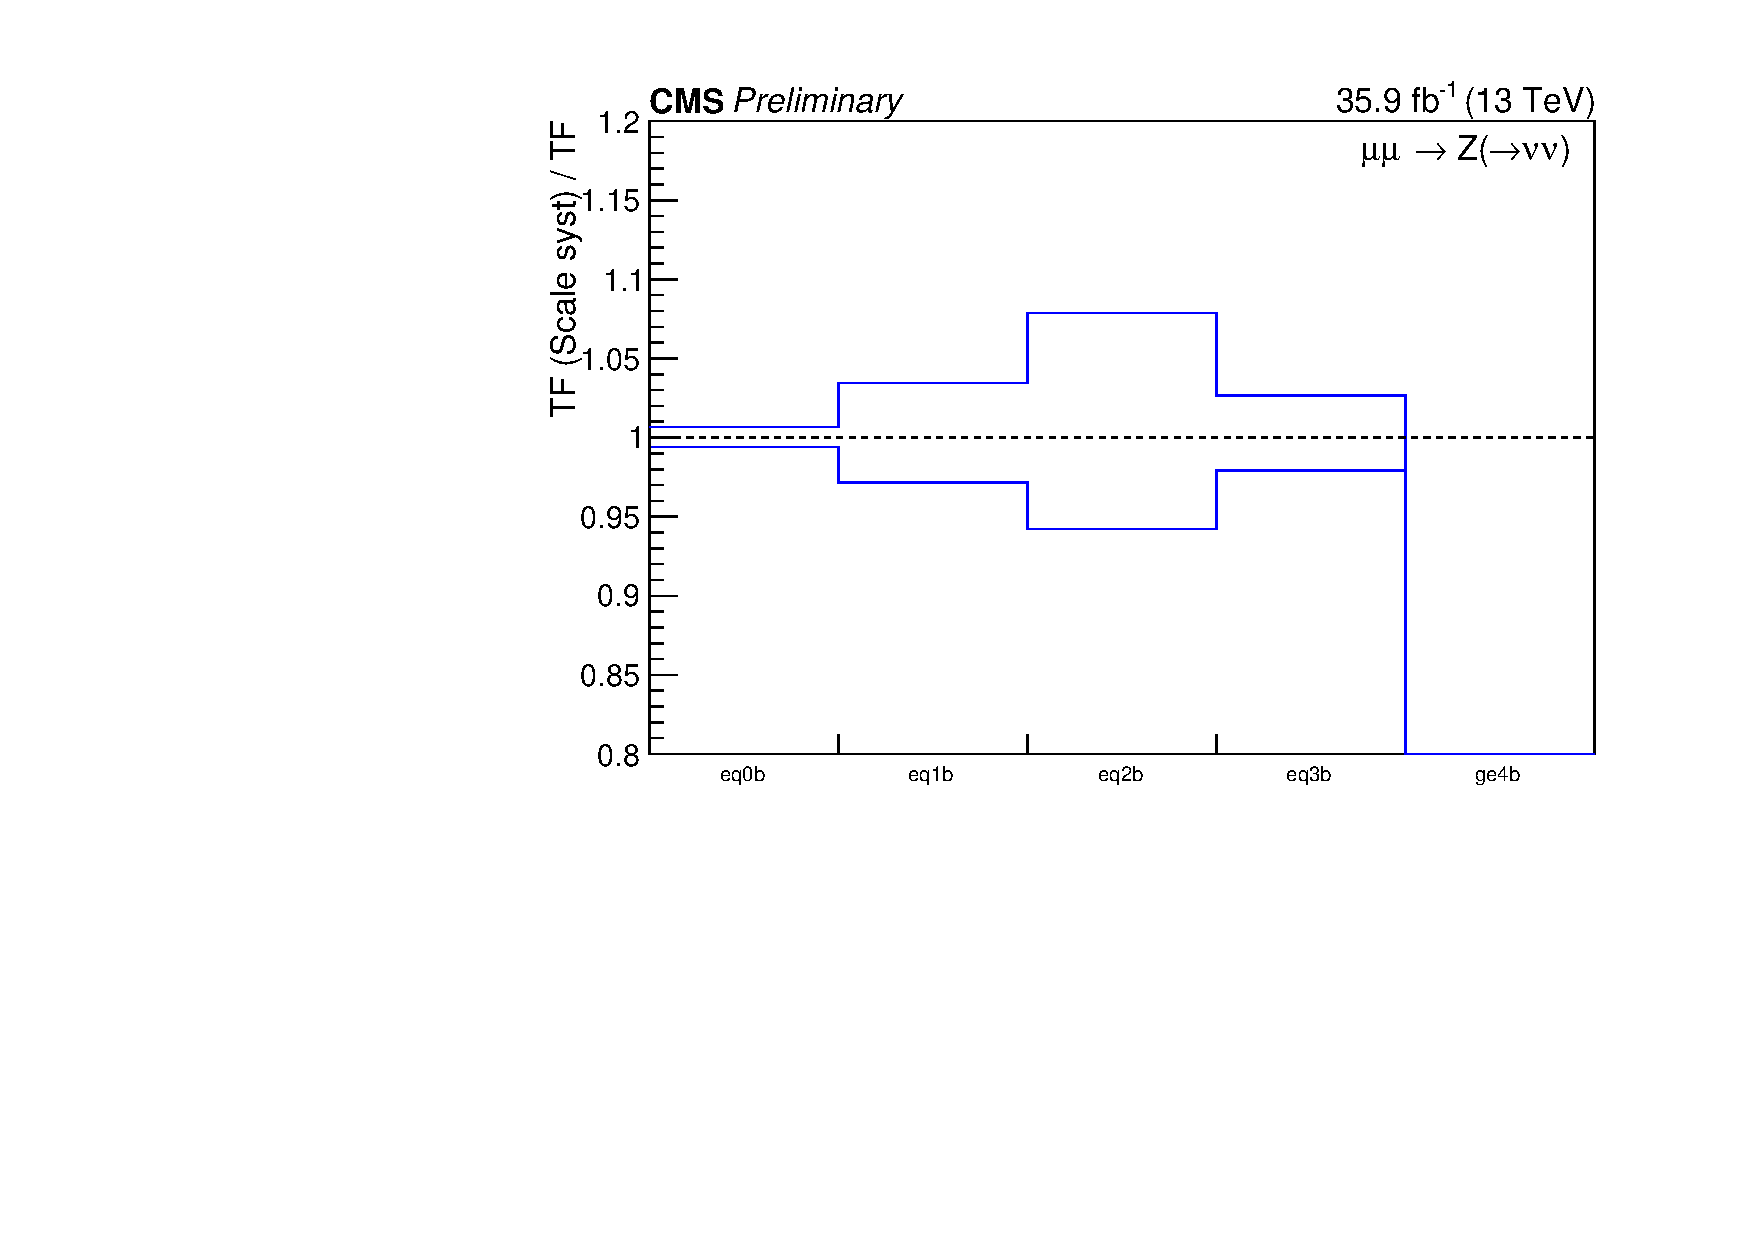
\includegraphics[width=0.5\textwidth]{figures/mcSystematics36p4fb/plots/tfratio_mumu_Zinv_bjet_scaleWeightUp.pdf}
  } ~
  \subfigure[Up/down variations versus \mht.]{
    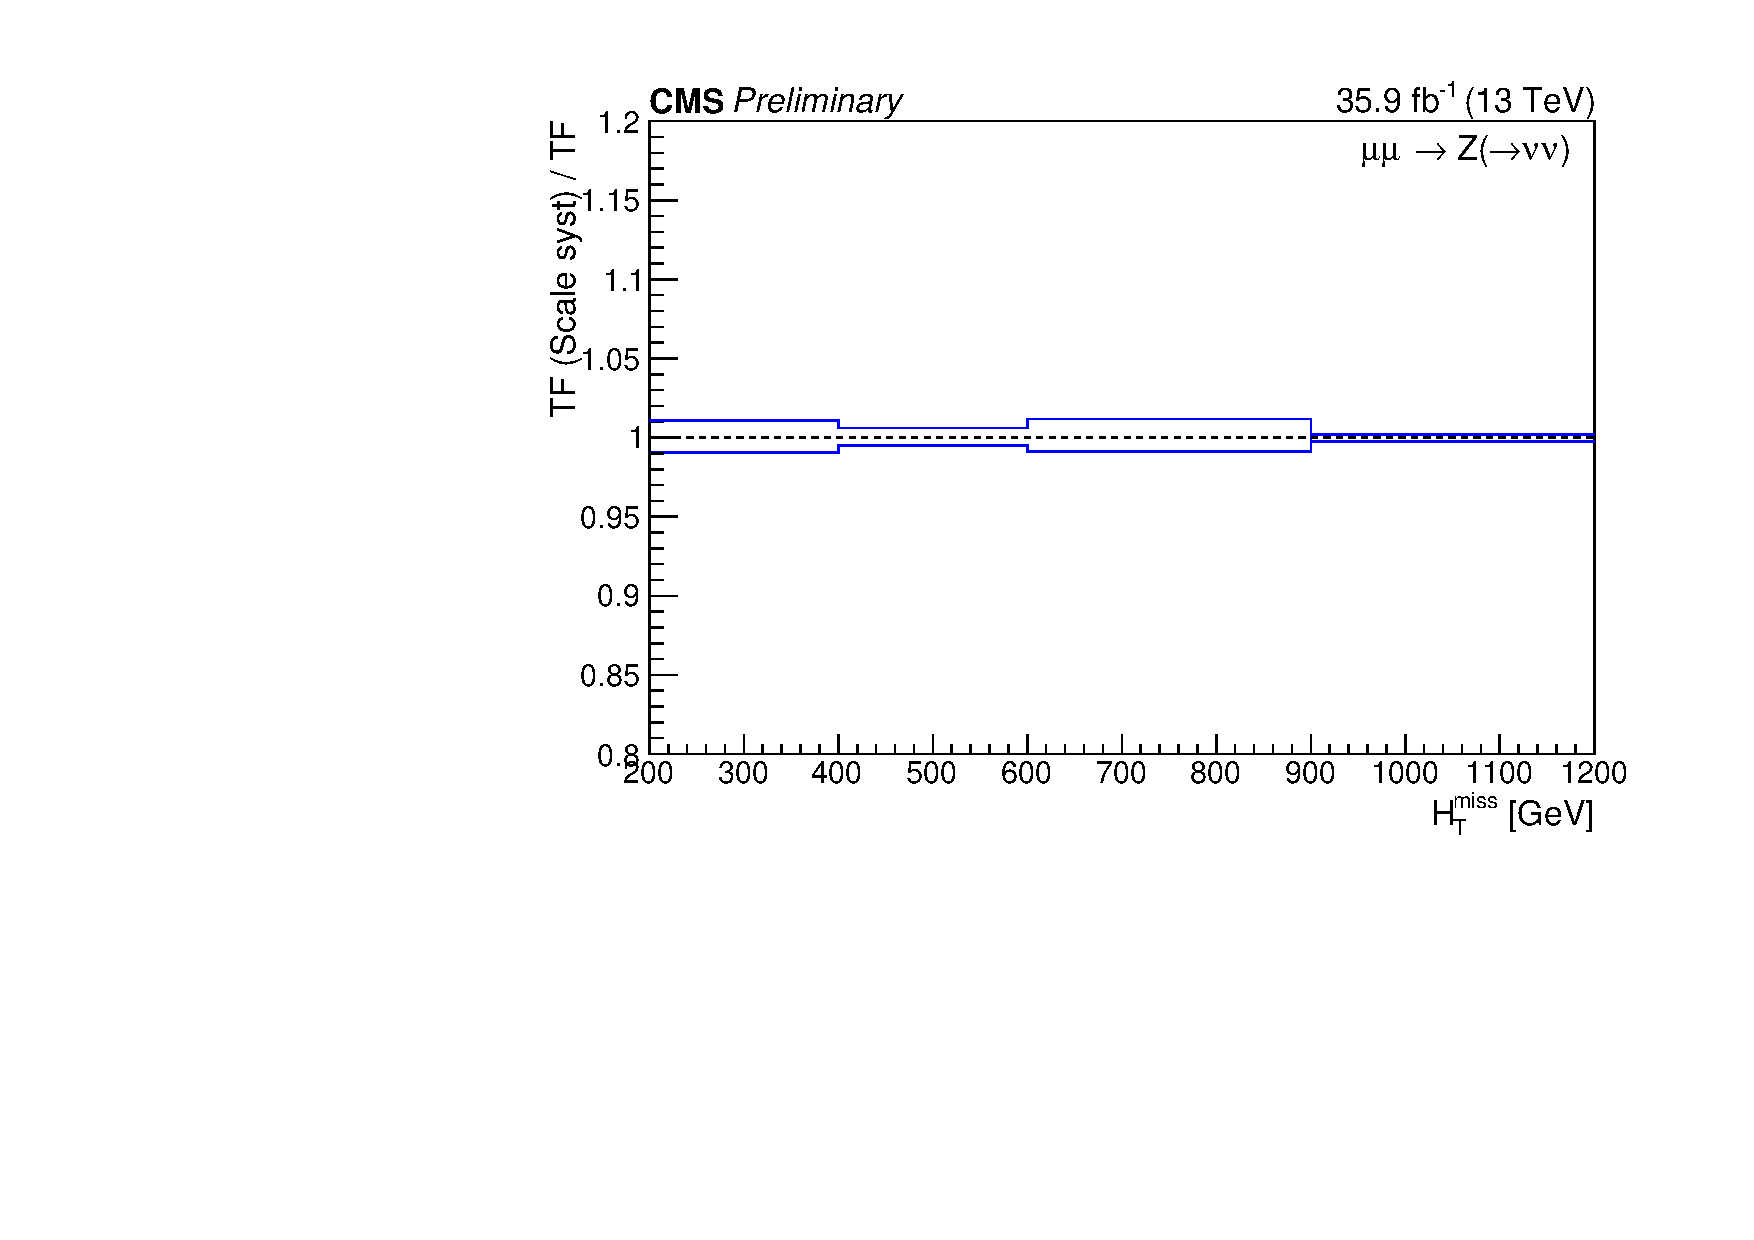
\includegraphics[width=0.5\textwidth]{figures/mcSystematics36p4fb/plots/tfratio_mumu_Zinv_mht_scaleWeightUp.pdf}
  } \\
  \caption{\label{fig:tfSyst_scale_mmZinv} The relative change in the
    ``$\mmj \rightarrow \znunu\ + \textrm{jets}$'' transfer factors from
    simulation due to $\pm1\sigma$ uncertainties in
    renormalisation/factorisation scales.  }
\end{figure}

\clearpage
\begin{figure}[!h]
  \centering
  \subfigure[Up variation versus (\njet,\nb) category and \scalht.]{
    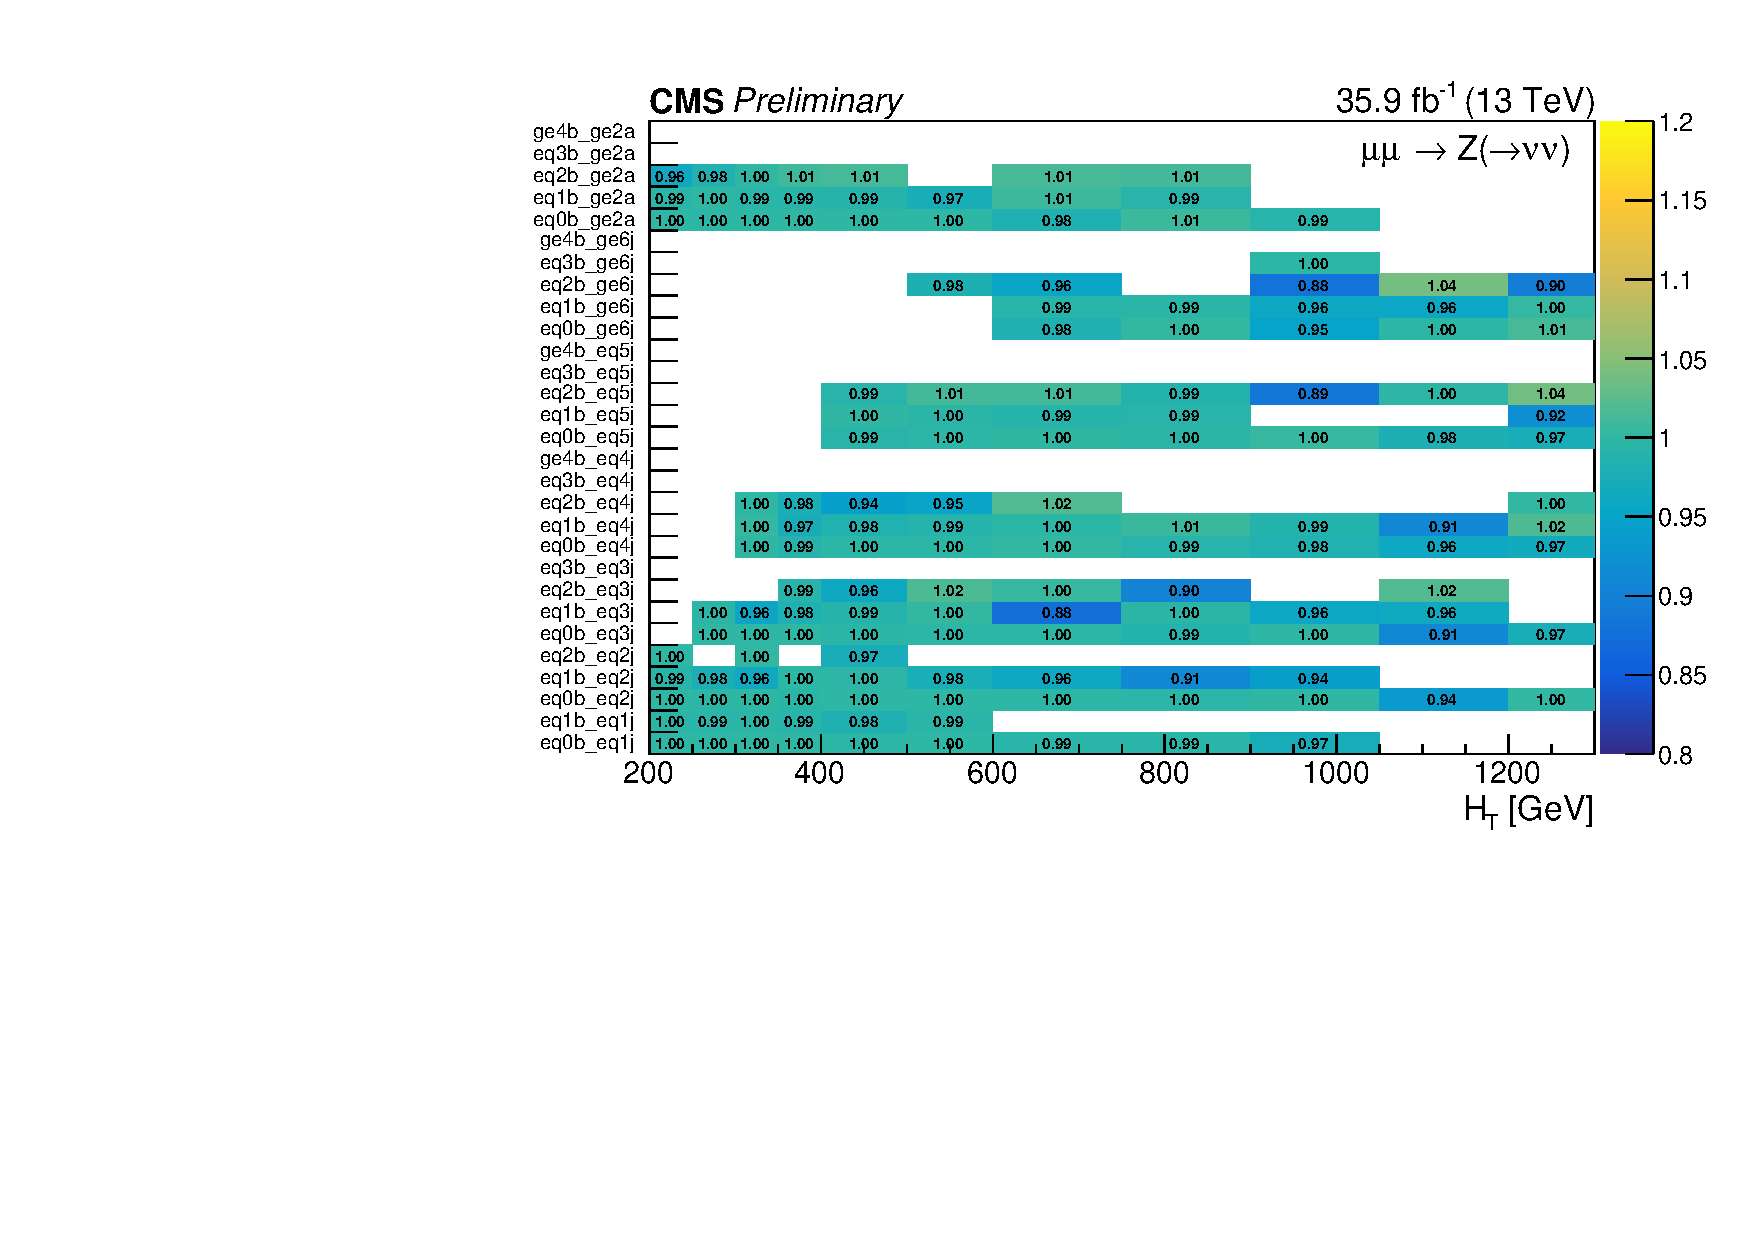
\includegraphics[width=0.5\textwidth]{figures/mcSystematics36p4fb/plots/tfratio_mumu_Zinv_2d_pdfWeightUp.pdf}
  } ~
  \subfigure[Down variation versus (\njet,\nb) category and \scalht.]{
    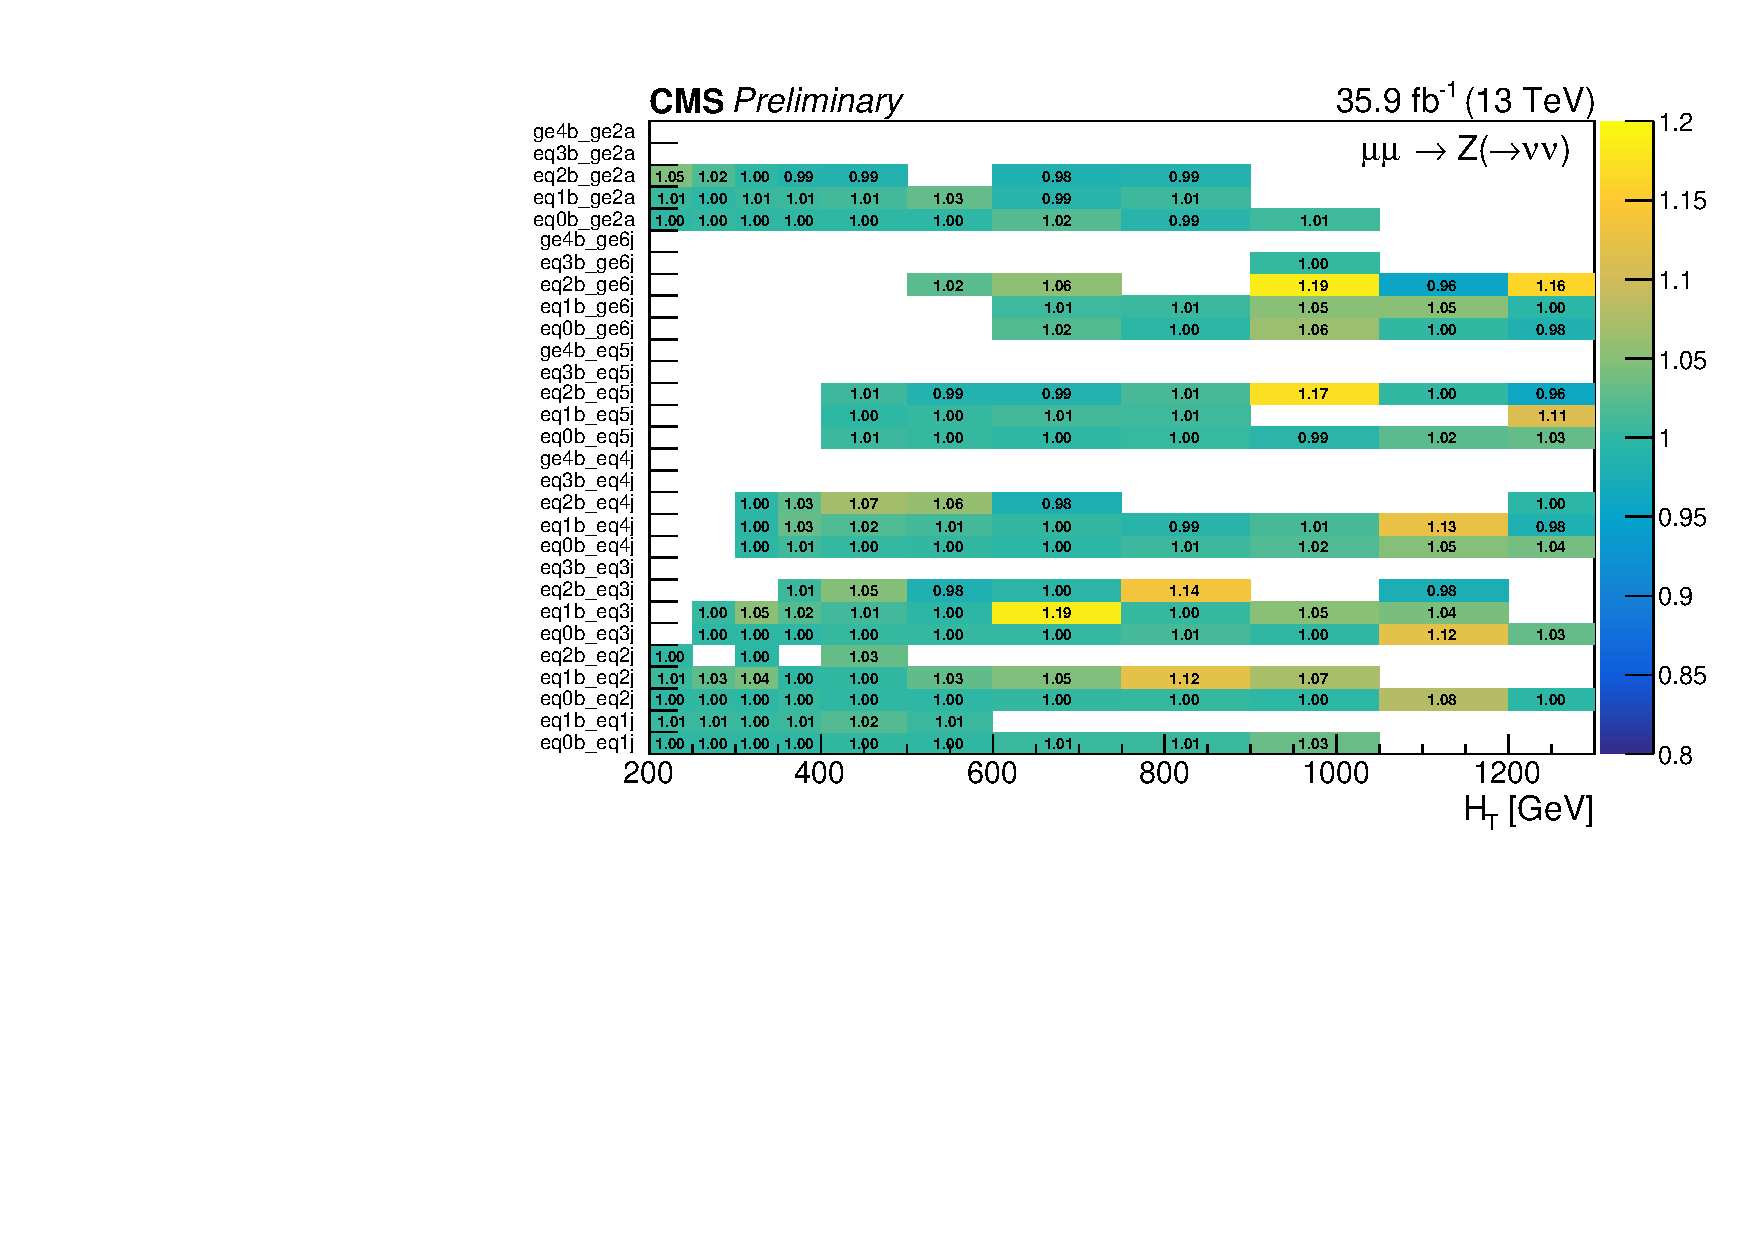
\includegraphics[width=0.5\textwidth]{figures/mcSystematics36p4fb/plots/tfratio_mumu_Zinv_2d_pdfWeightDown.pdf}
  }\\
  \subfigure[Up/down variations versus \njet.]{
    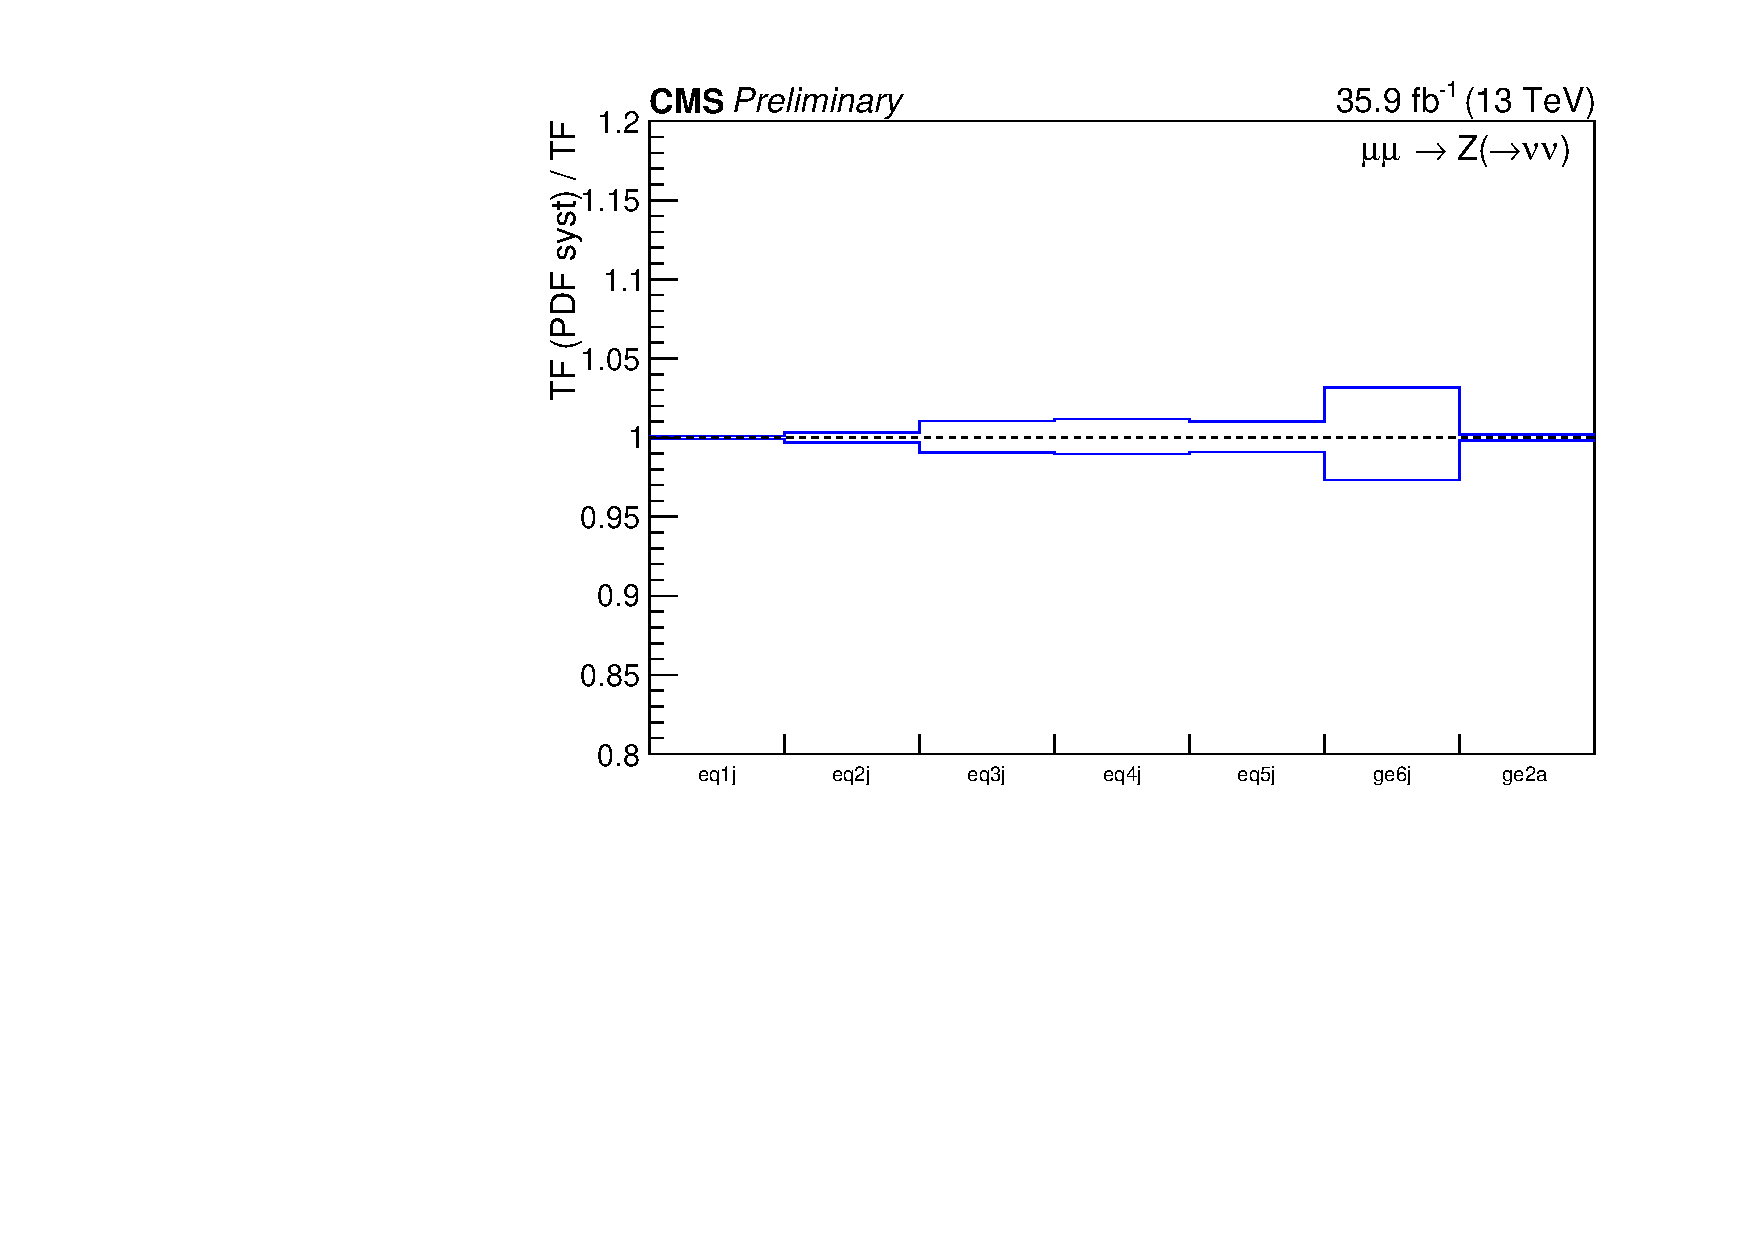
\includegraphics[width=0.5\textwidth]{figures/mcSystematics36p4fb/plots/tfratio_mumu_Zinv_njet_pdfWeightUp.pdf}
  } ~
  \subfigure[Up/down variations versus \scalht.]{
    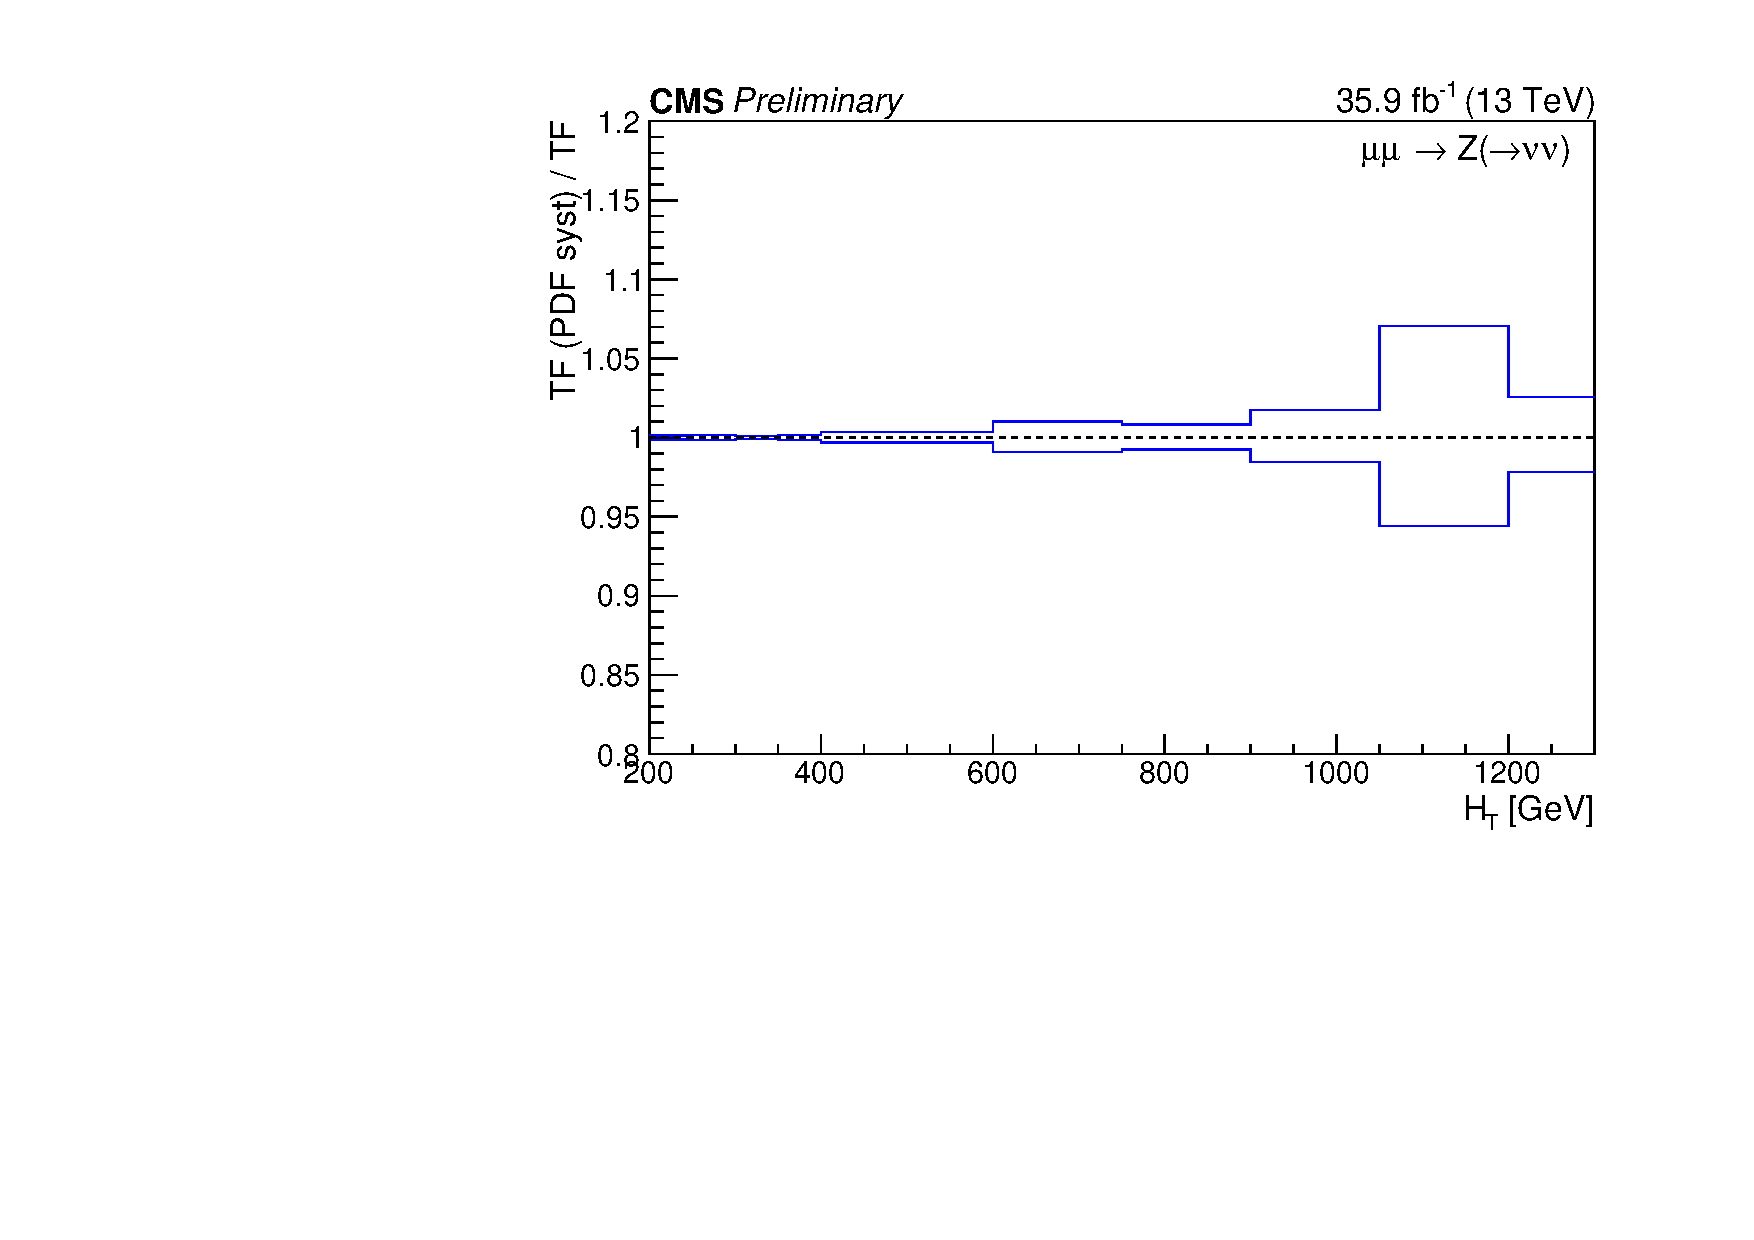
\includegraphics[width=0.5\textwidth]{figures/mcSystematics36p4fb/plots/tfratio_mumu_Zinv_ht_pdfWeightUp.pdf}
  } \\
  \subfigure[Up/down variations versus \nb.]{
    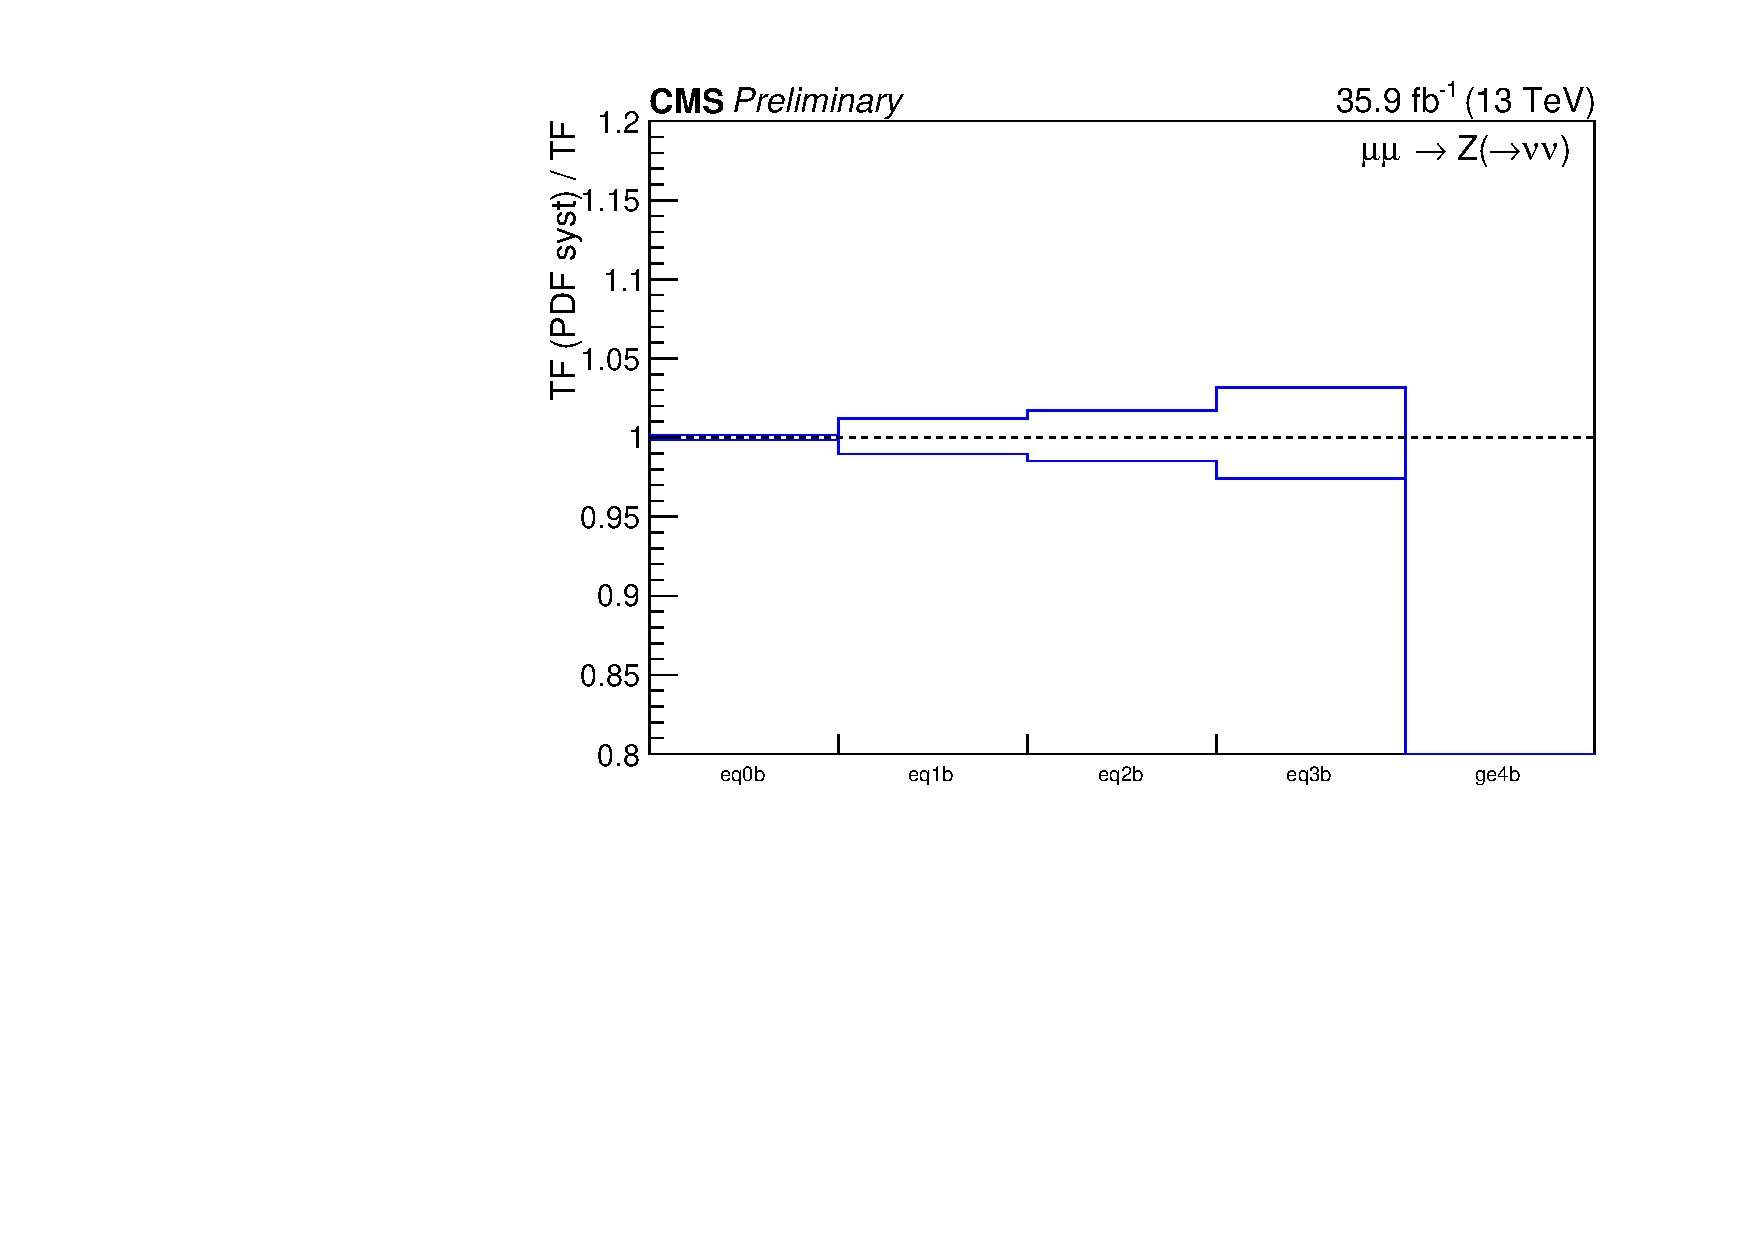
\includegraphics[width=0.5\textwidth]{figures/mcSystematics36p4fb/plots/tfratio_mumu_Zinv_bjet_pdfWeightUp.pdf}
  } ~
  \subfigure[Up/down variations versus \mht.]{
    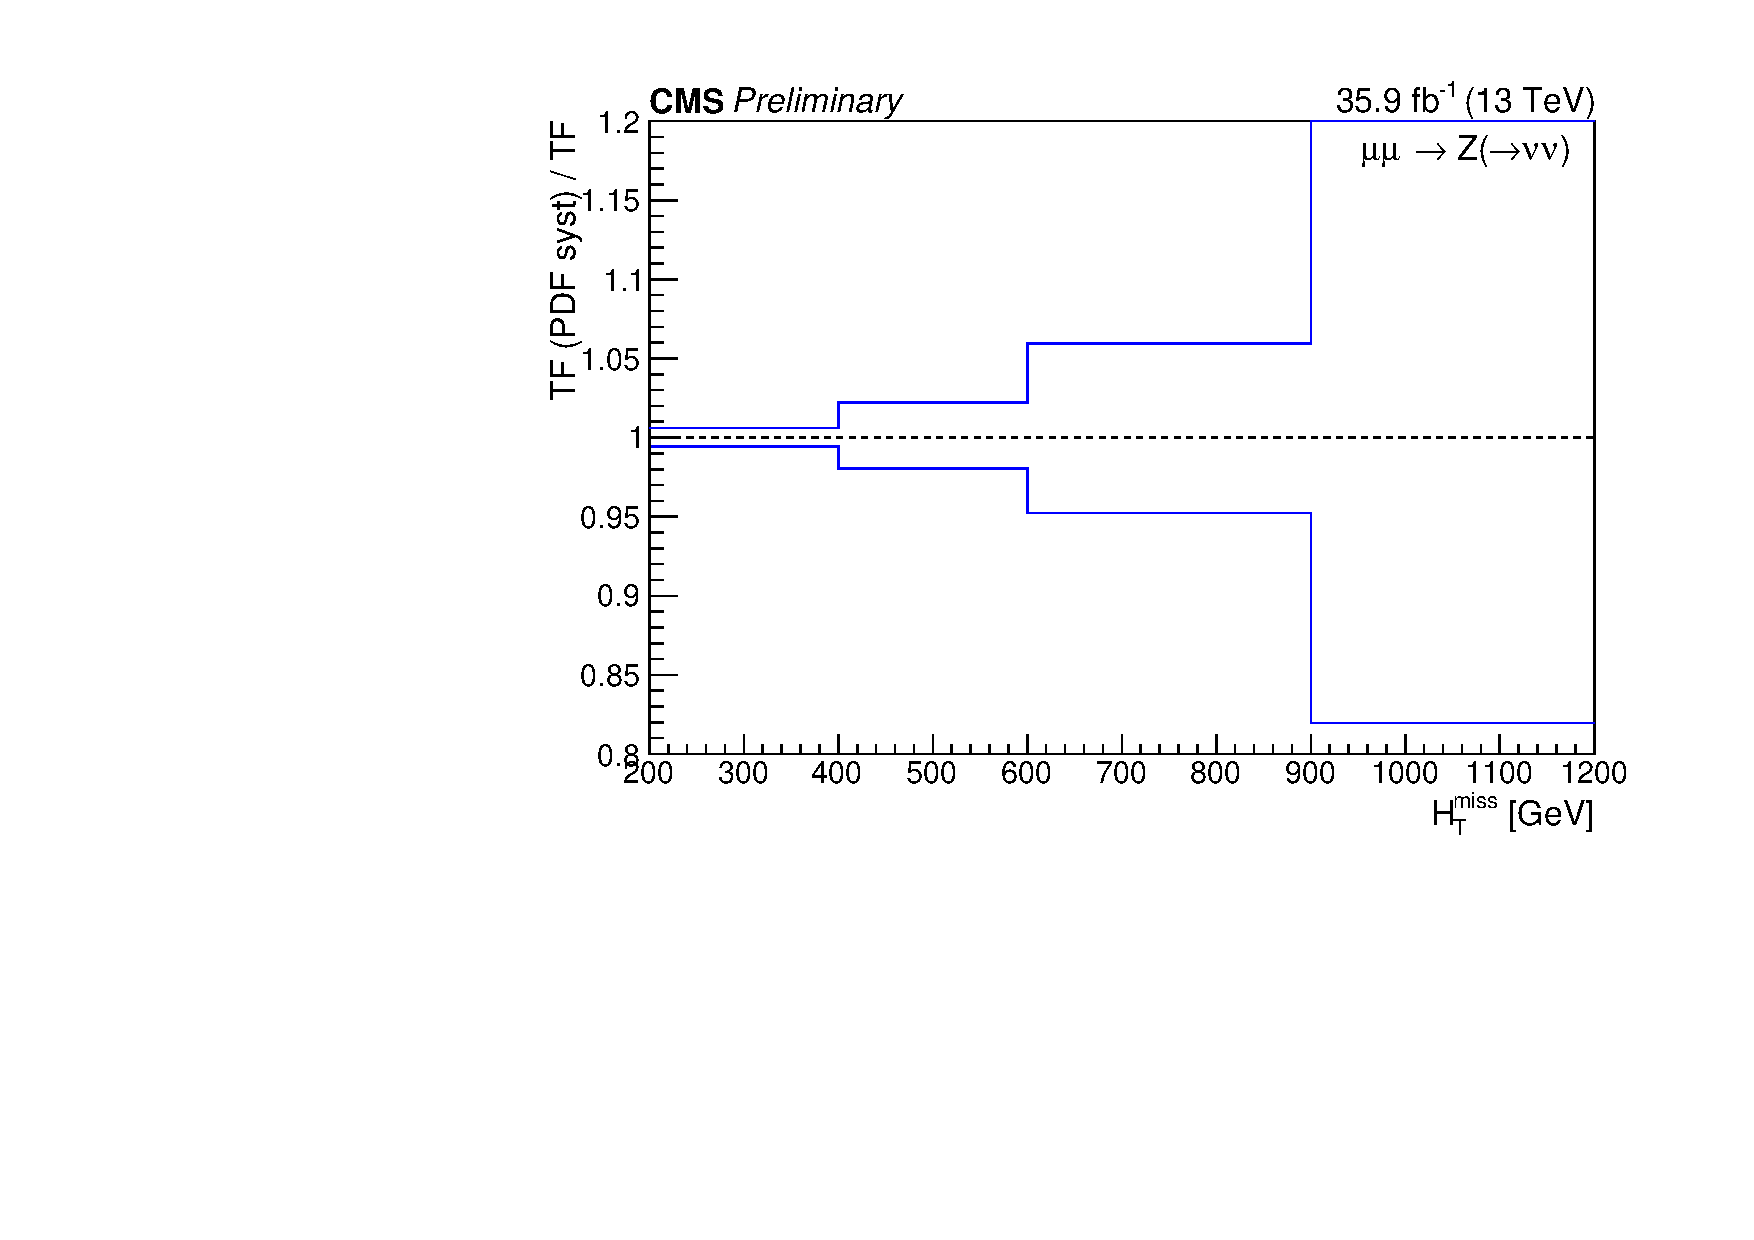
\includegraphics[width=0.5\textwidth]{figures/mcSystematics36p4fb/plots/tfratio_mumu_Zinv_mht_pdfWeightUp.pdf}
  } \\
  \caption{\label{fig:tfSyst_pdf_mmZinv} The relative change in the
    ``$\mmj \rightarrow \znunu\ + \textrm{jets}$'' transfer factors from
    simulation due to $\pm1\sigma$ uncertainties in parton density
    functions.  } 
\end{figure}

\clearpage
\subsection{Missing higher-order corrections in LO \texorpdfstring{\MADGRAPH}{MadGraph}
  samples}
  In addition to the figures below, the plots in figure~\ref{fig:NLO_app} are also relevant.

\begin{figure}[!h]
  \centering
  \subfigure[Correction versus Z boson \Pt.]{
    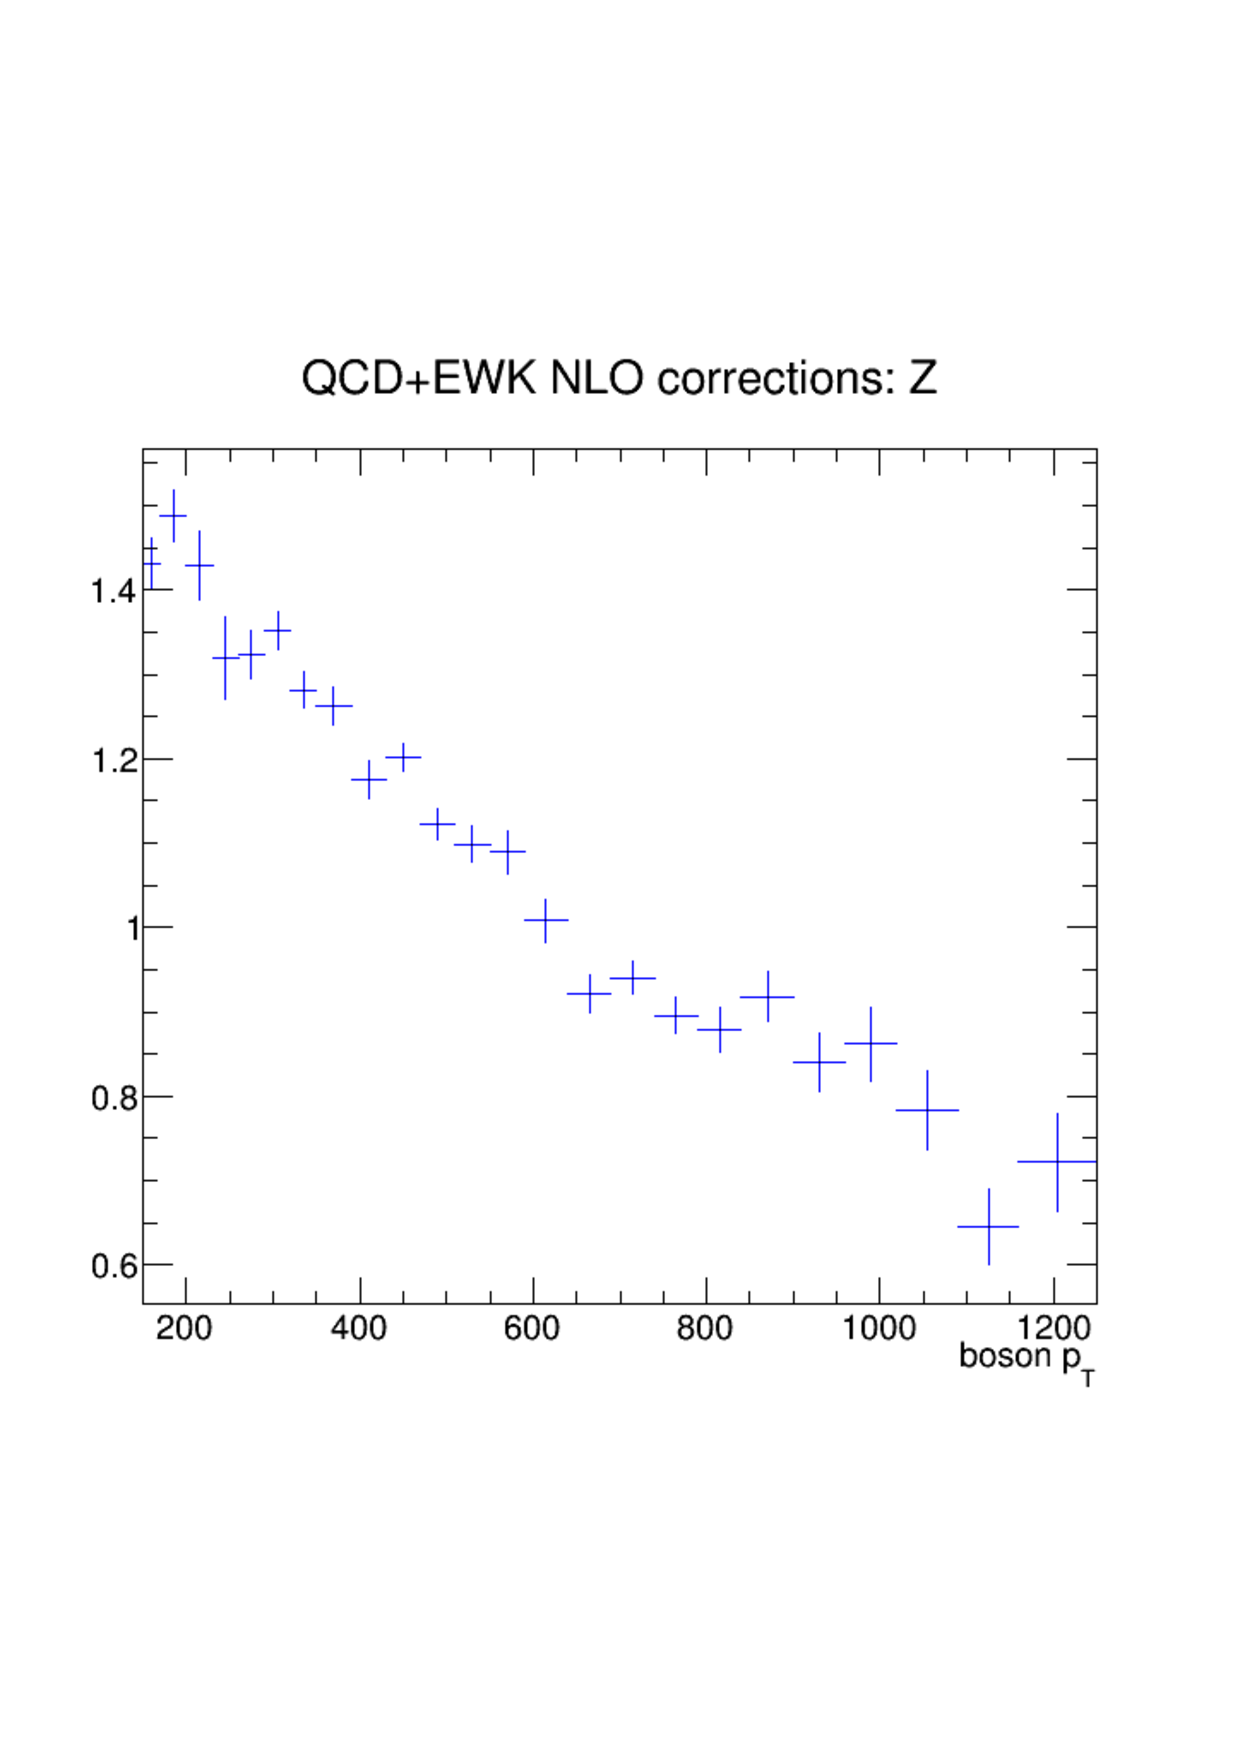
\includegraphics[width=0.4\textwidth,trim=0 150 0 150]{figures/NLO/Z.pdf}
  } ~
  \subfigure[Variation versus (\njet,\nb) category and \scalht.]{
    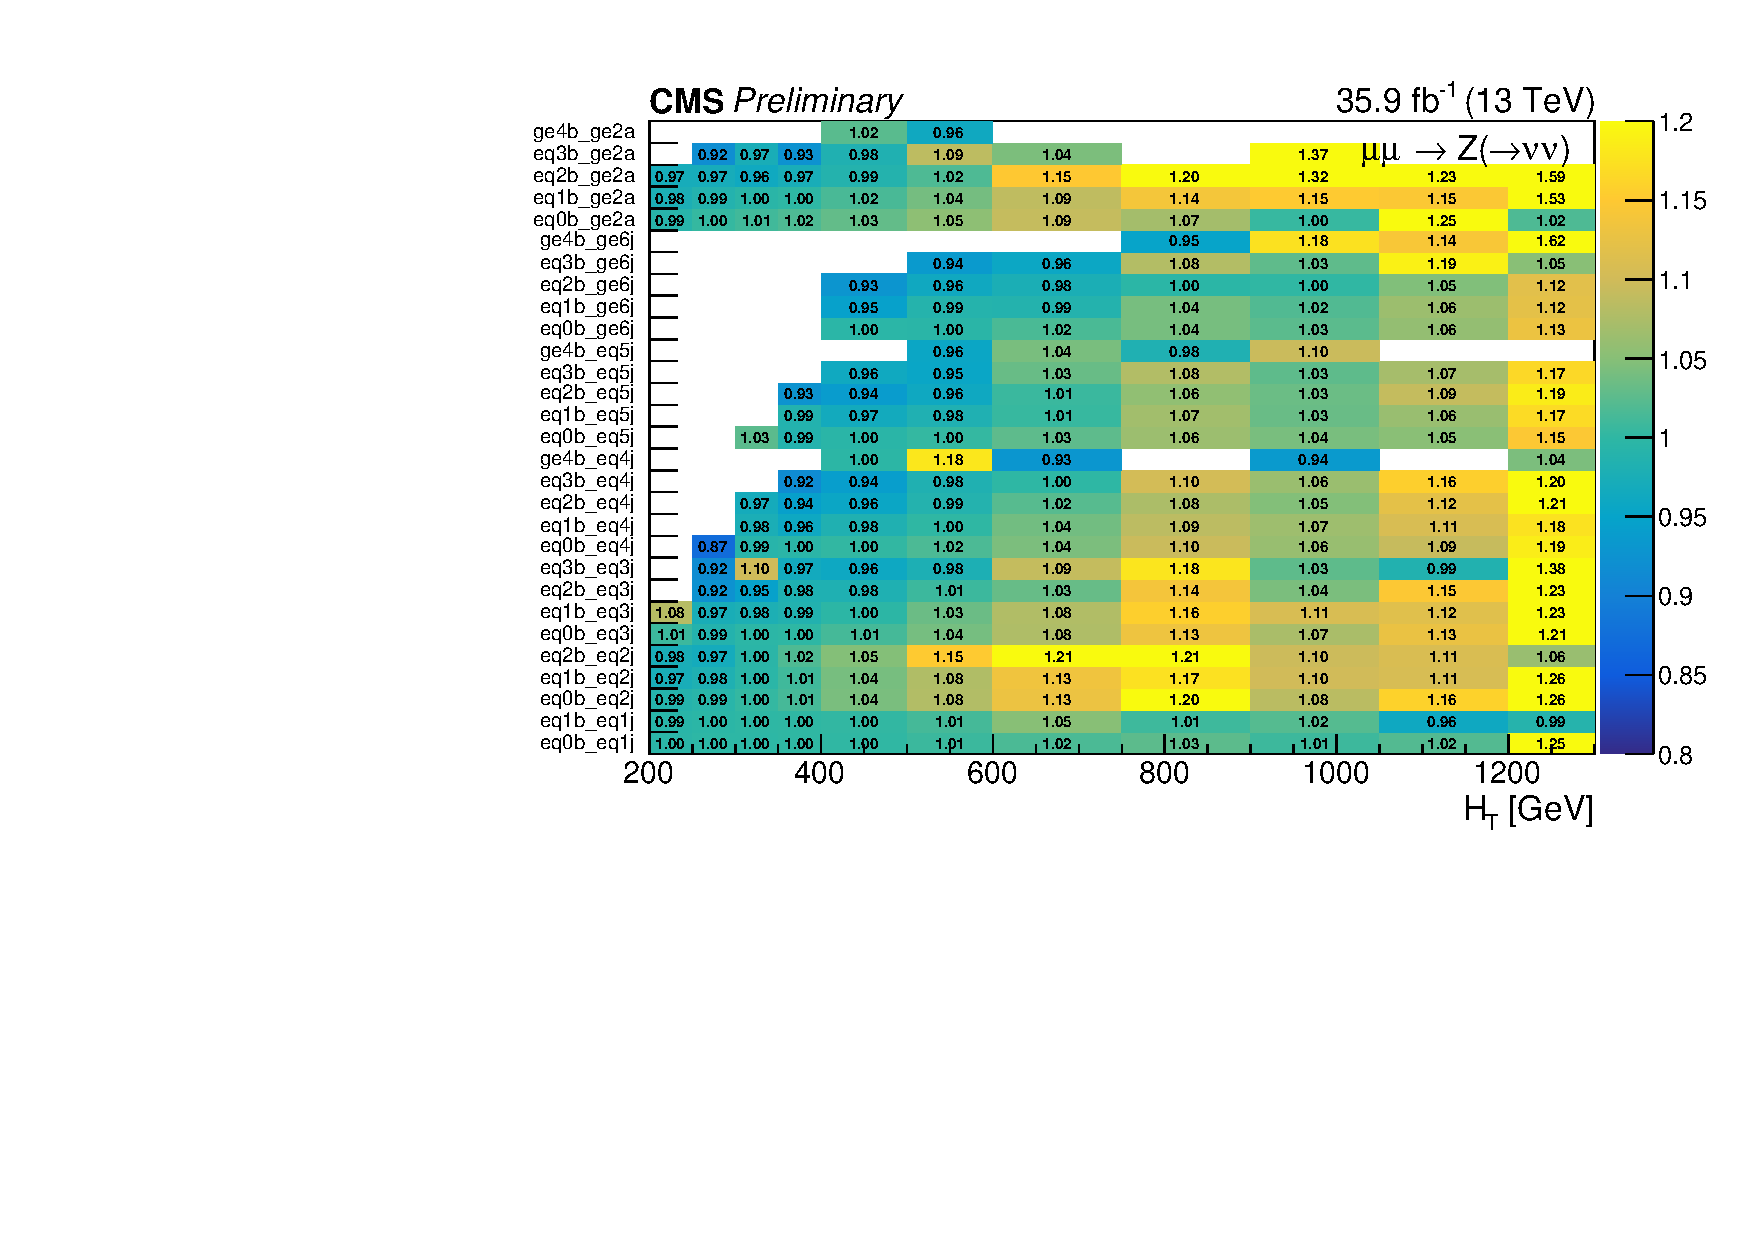
\includegraphics[width=0.5\textwidth]{figures/mcSystematics36p4fb/plots/tfratio_mumu_Zinv_2d_bosonPtWeightDown.pdf}
  }\\
  \subfigure[Variation versus \njet.]{
    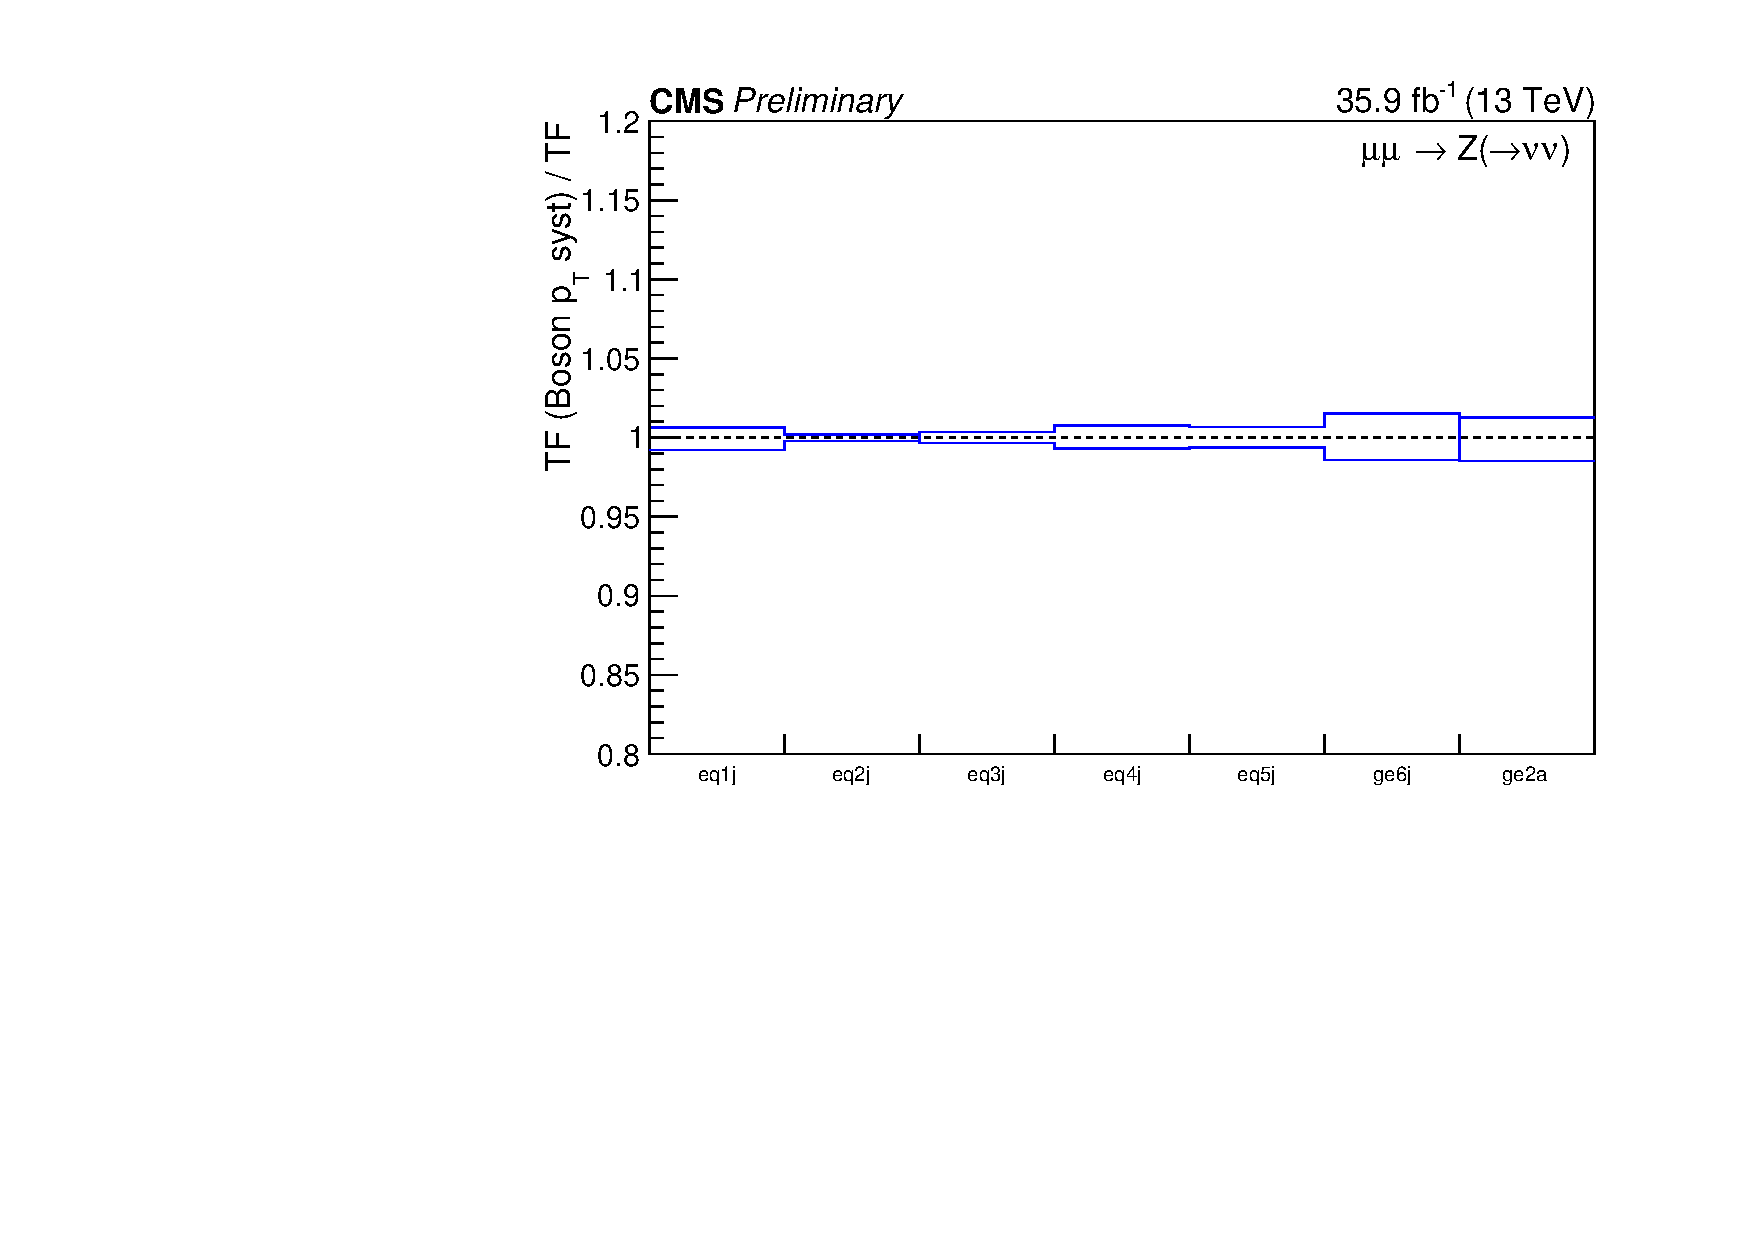
\includegraphics[width=0.5\textwidth]{figures/mcSystematics36p4fb/plots/tfratio_mumu_Zinv_njet_bosonPtWeightUp.pdf}
  } ~
  \subfigure[Variation versus \scalht.]{
    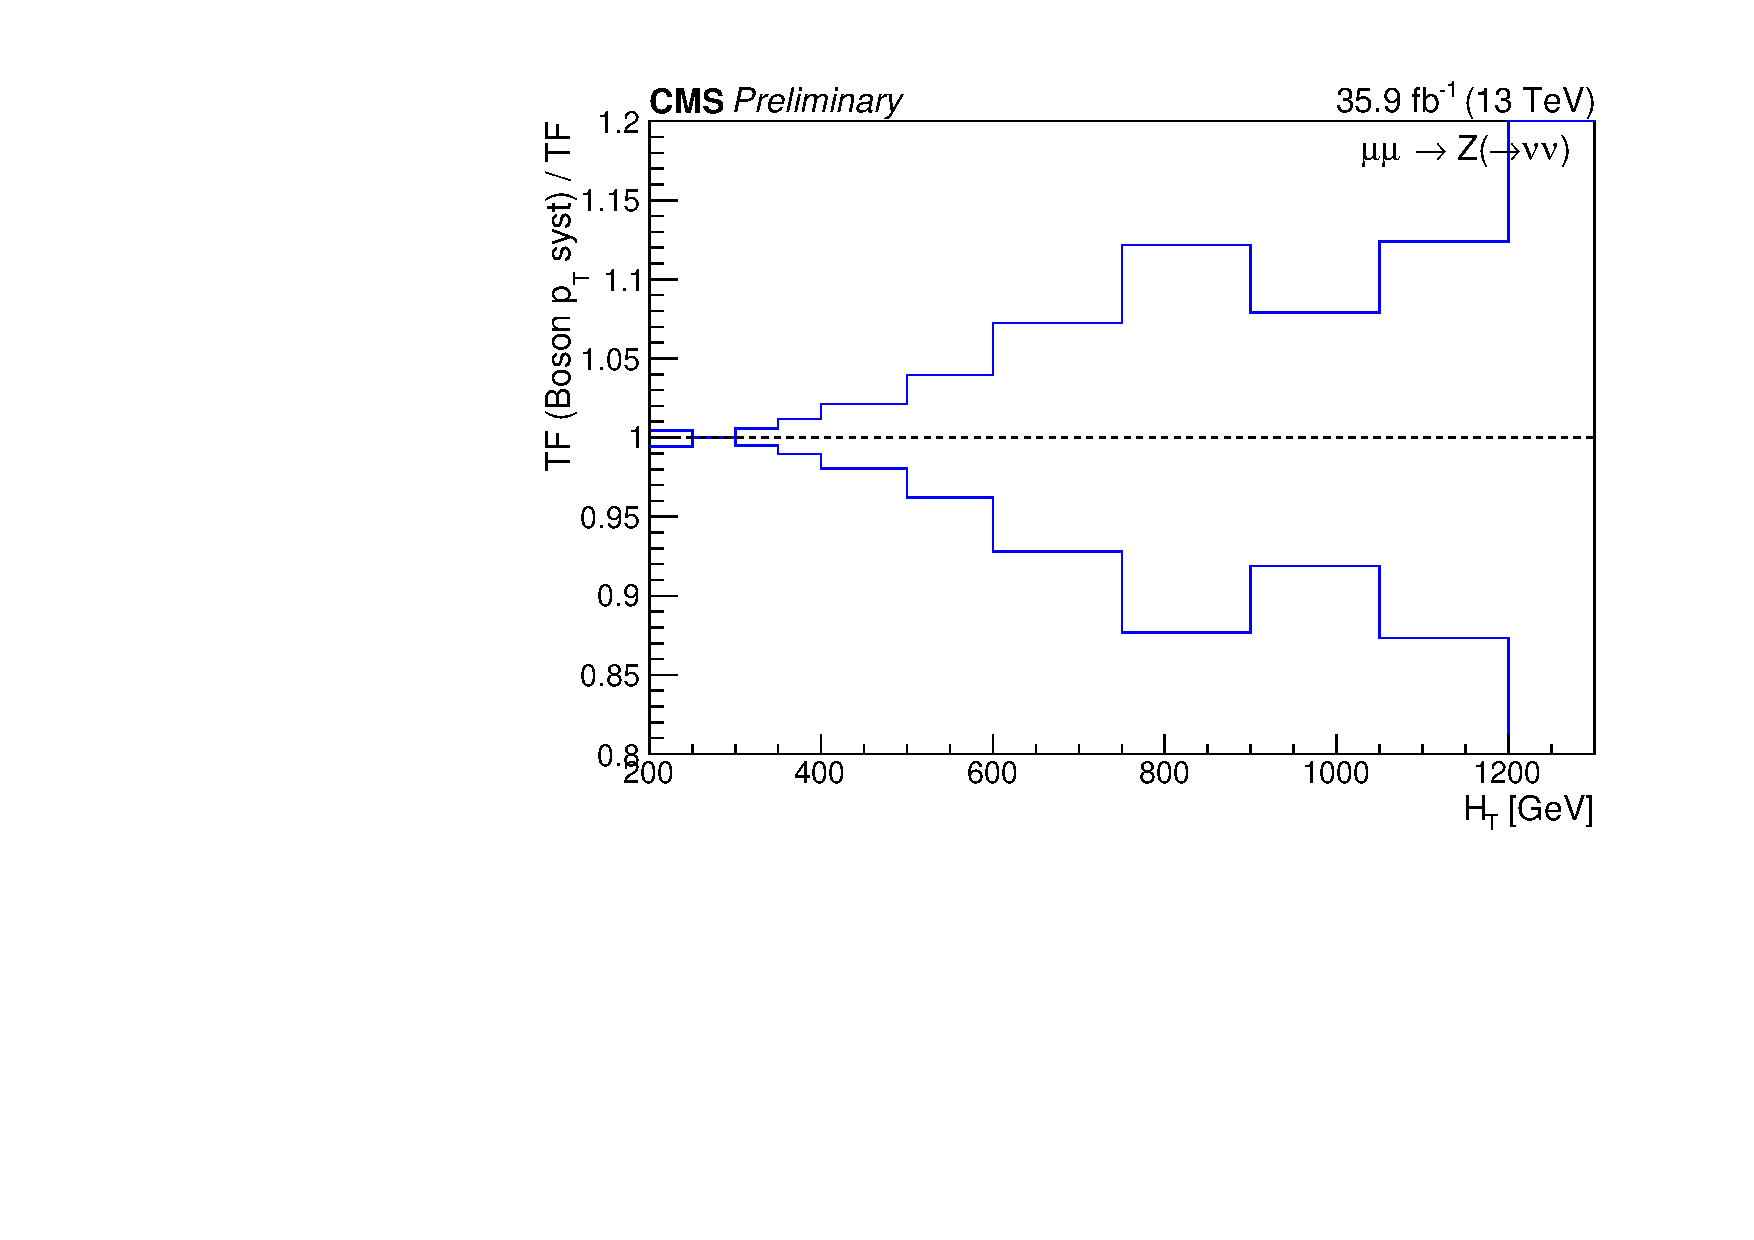
\includegraphics[width=0.5\textwidth]{figures/mcSystematics36p4fb/plots/tfratio_mumu_Zinv_ht_bosonPtWeightUp.pdf}
  } \\
  \subfigure[Variation versus \nb.]{
    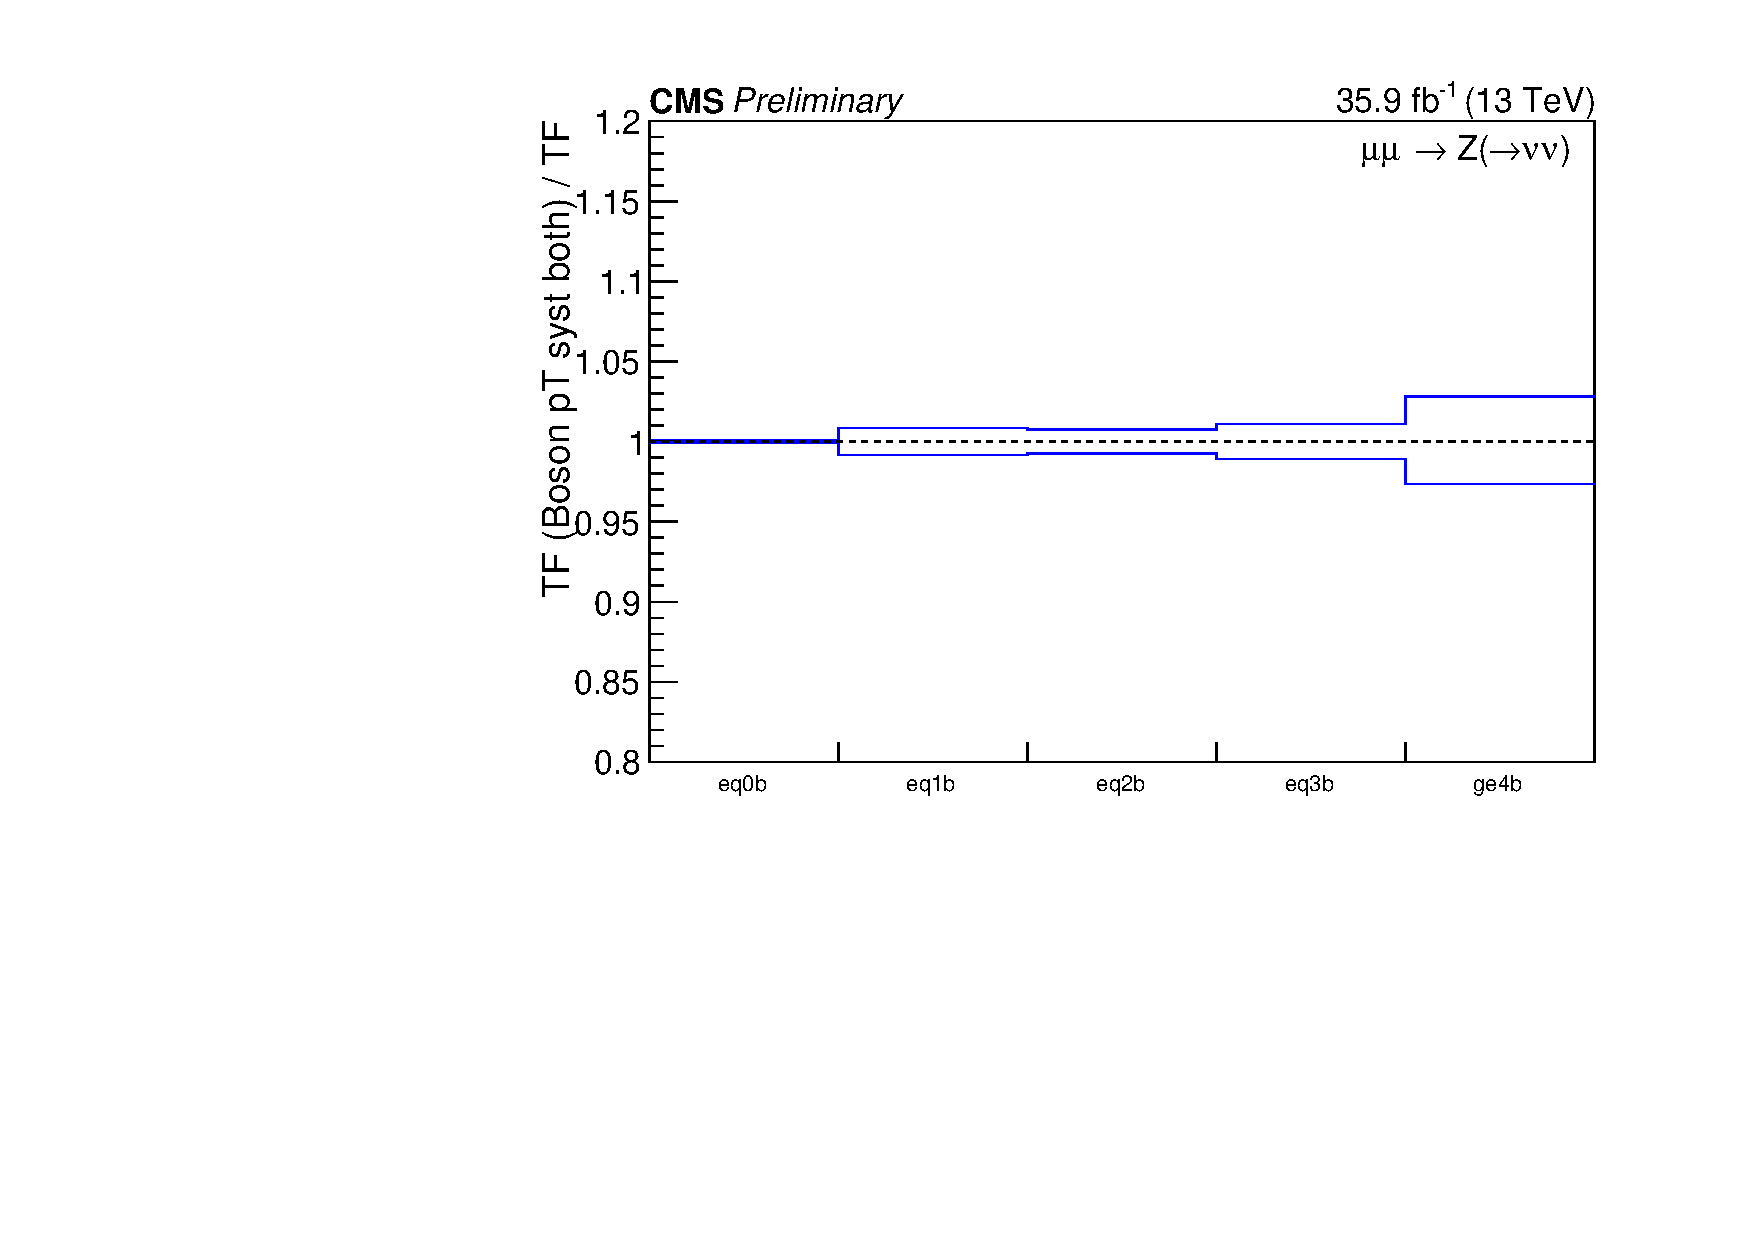
\includegraphics[width=0.5\textwidth]{figures/mcSystematics36p4fb/plots/tfratio_mumu_Zinv_bjet_bosonPtWeightUp.pdf}
  } ~
  \subfigure[Variation versus \mht.]{
    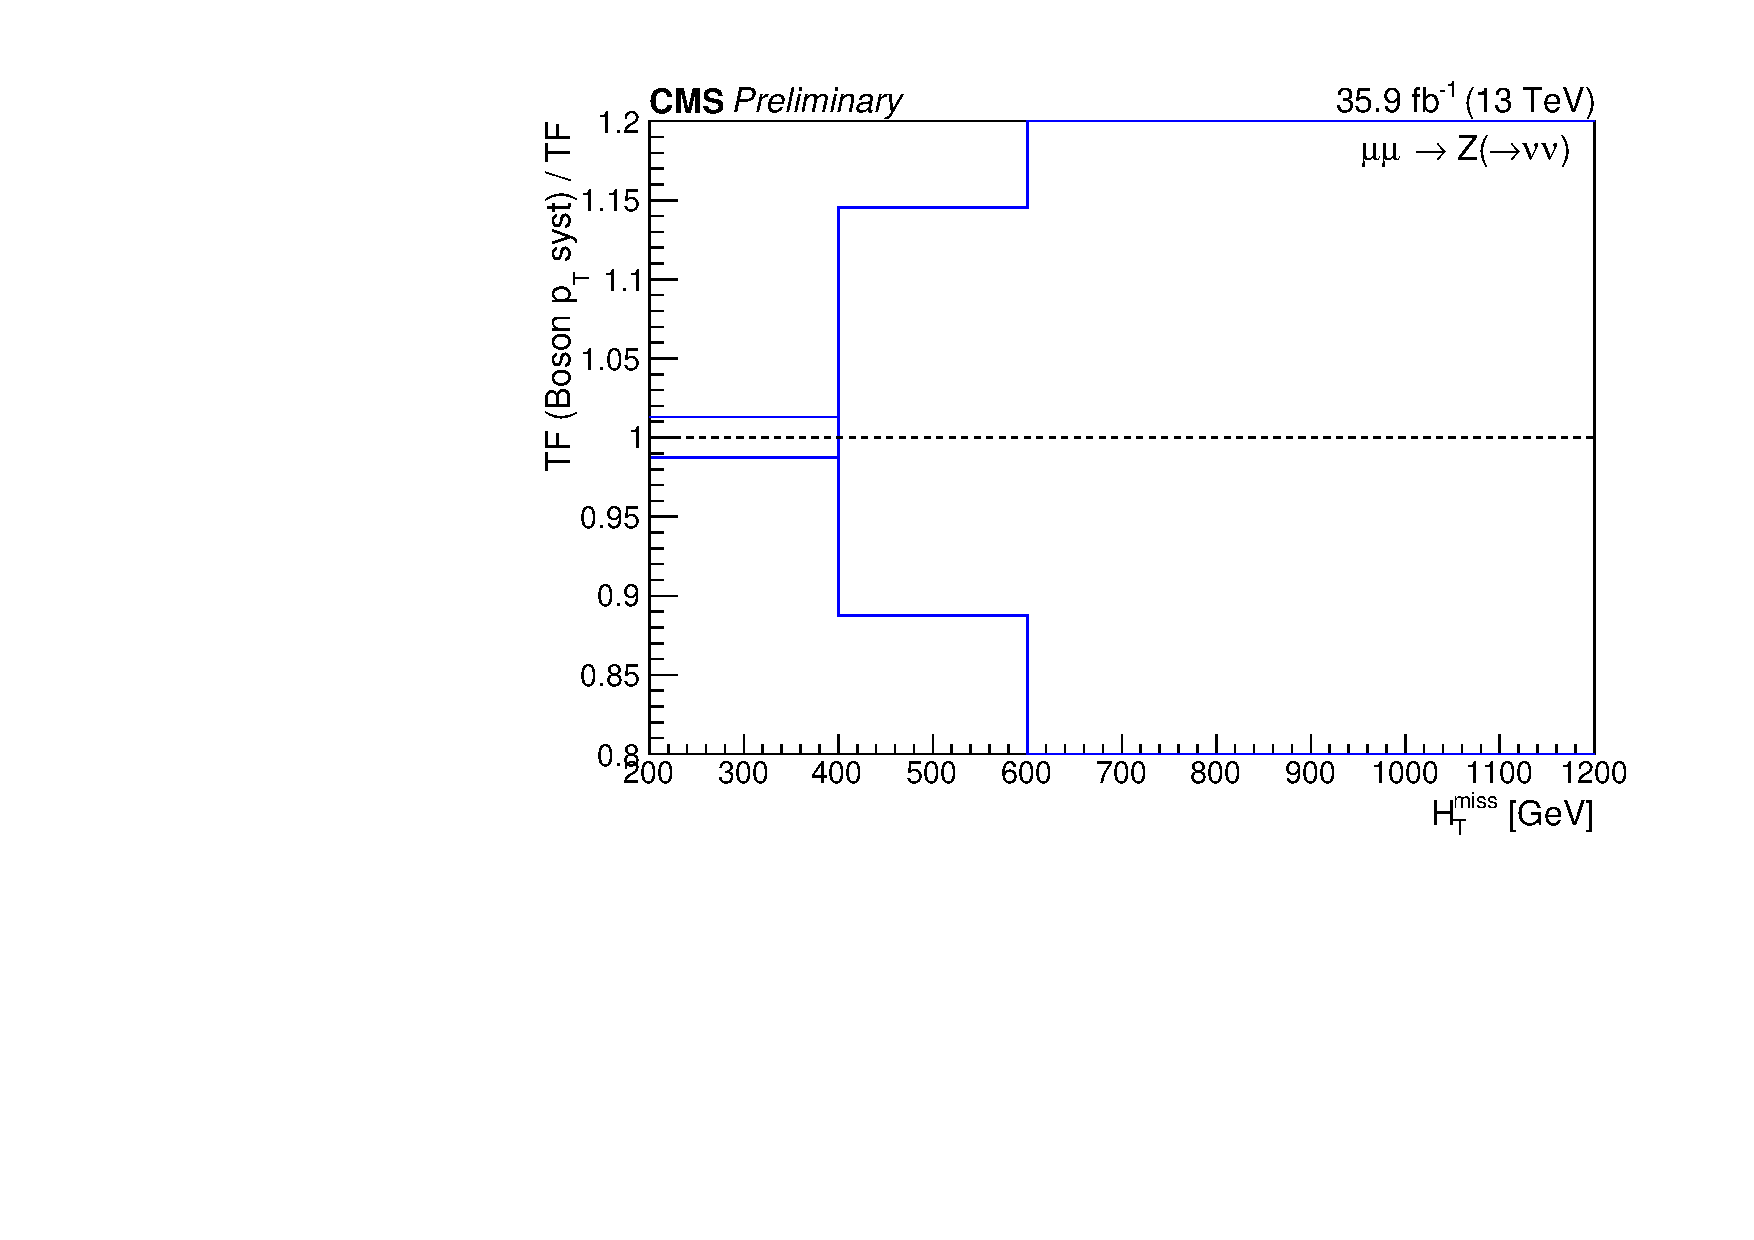
\includegraphics[width=0.5\textwidth]{figures/mcSystematics36p4fb/plots/tfratio_mumu_Zinv_mht_bosonPtWeightUp.pdf}
  } \\
  \caption{\label{fig:tfSyst_nlo_mmZinv} The relative change in the
    ``$\mmj \rightarrow \znunu\ + \textrm{jets}$'' transfer factors from
    simulation when assuming uncertainties equal in magnitude to QCD +
    EWK NLO corrections versus Z boson \Pt.  }
\end{figure}

%\clearpage
%\begin{figure}[!h]
%  \centering
%  \subfigure[\label{fig:NLO:mono-asymm}Monojet and asymmetric topologies]{
%    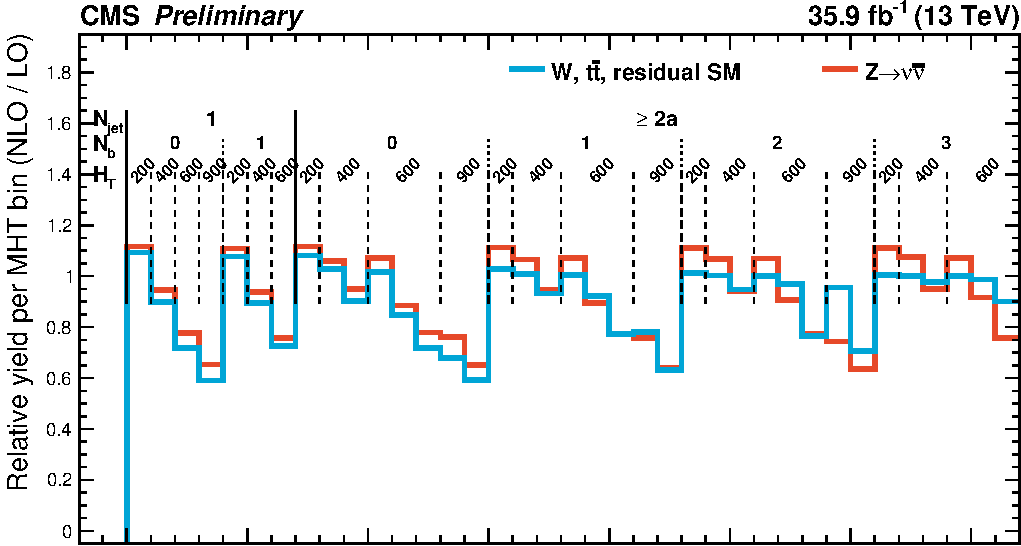
\includegraphics[width=0.48\textwidth]{figures/NLO/monojet_no-fit_NLO.pdf}
%  }~ 
%  \subfigure[\label{fig:NLO:dijet}Dijet topologies]{
%    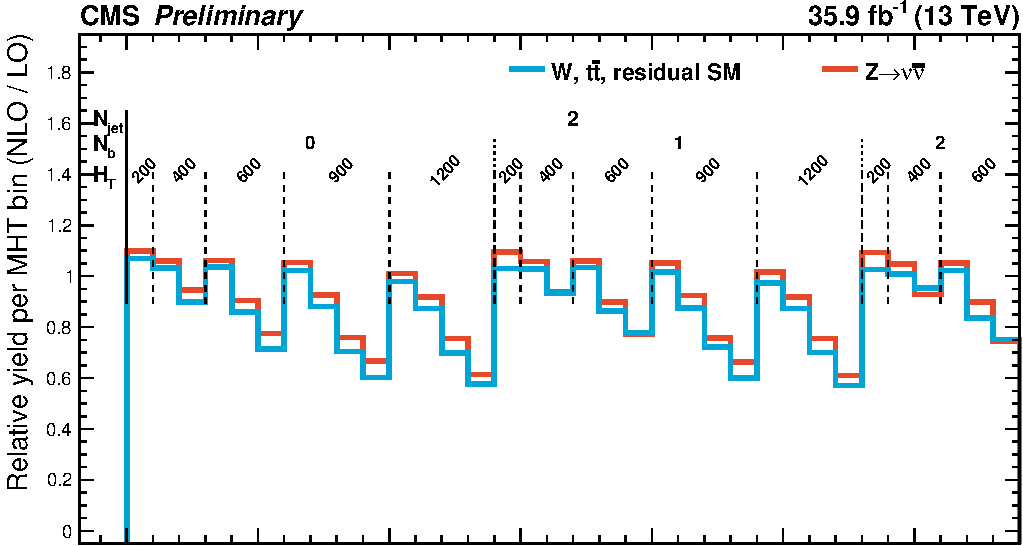
\includegraphics[width=0.48\textwidth]{figures/NLO/di-jet_no-fit_NLO.pdf}
%  }\\
%  \subfigure[\label{fig:NLO:three-jet}Topologies with 3 jets]{
%    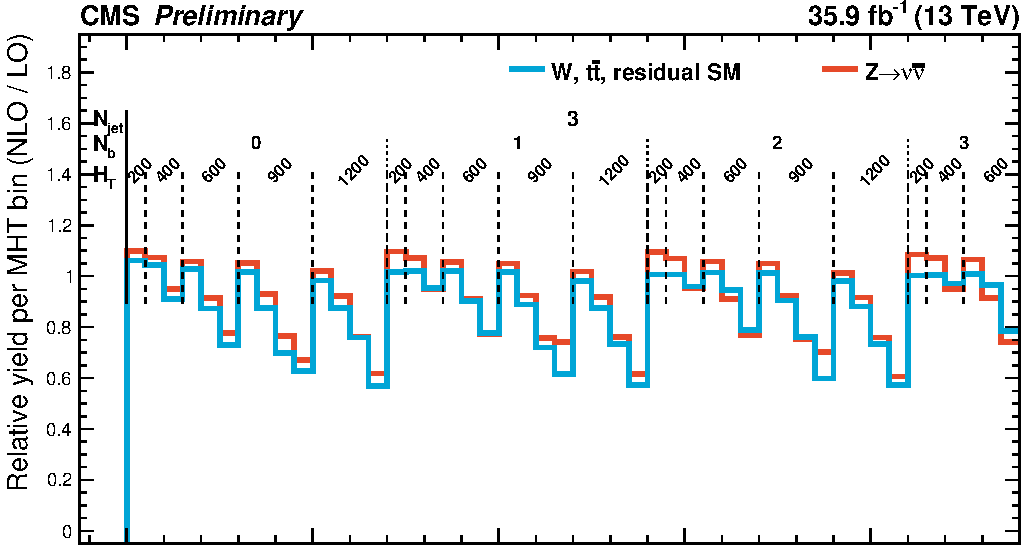
\includegraphics[width=0.48\textwidth]{figures/NLO/3jet_no-fit_NLO.pdf}
%  }~ 
%  \subfigure[\label{fig:NLO:four-jet}Topologies with 4 jets]{
%    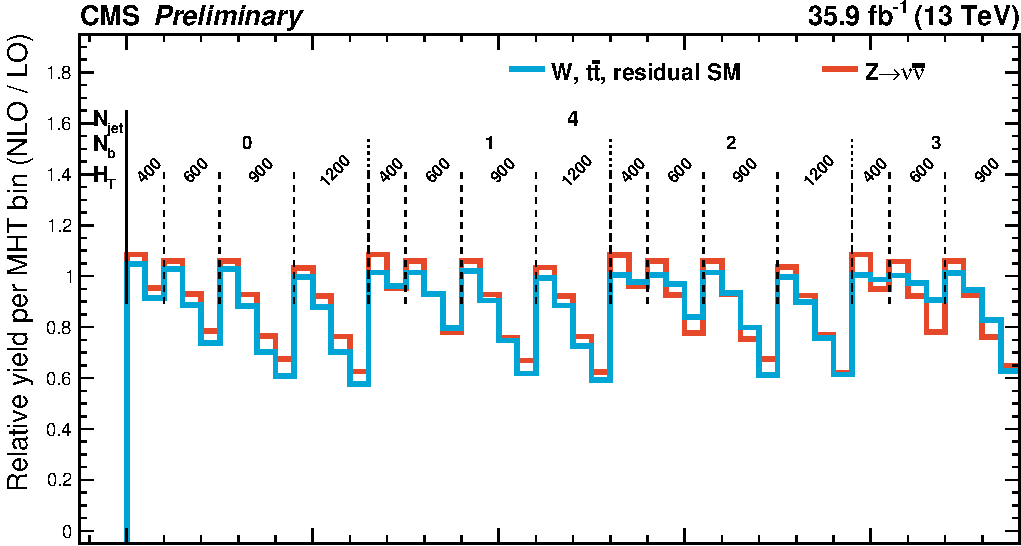
\includegraphics[width=0.48\textwidth]{figures/NLO/4jet_no-fit_NLO.pdf}
%  }\\
%  \subfigure[\label{fig:NLO:five-jet}Topologies with 5 jets]{
%    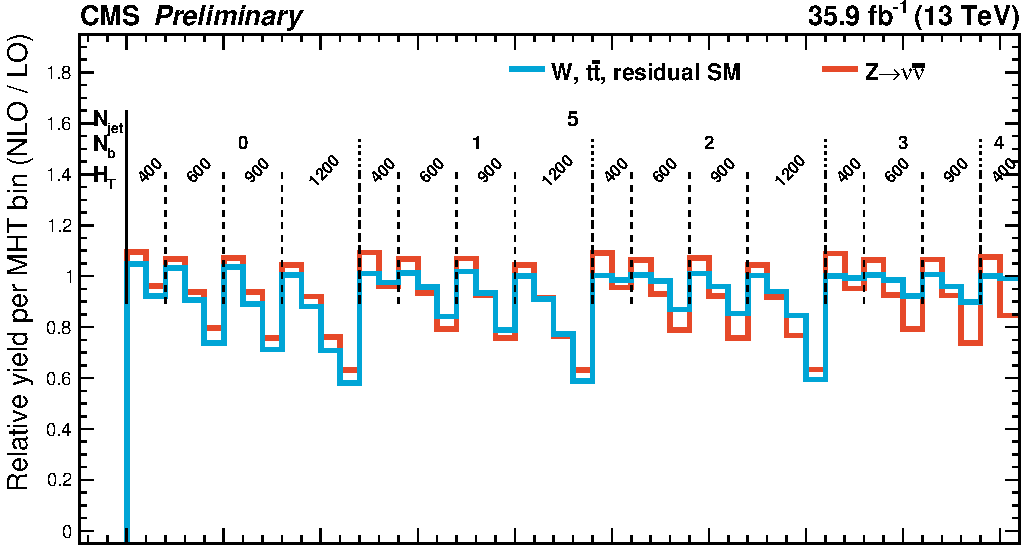
\includegraphics[width=0.48\textwidth]{figures/NLO/5jet_no-fit_NLO.pdf}
%  }~ 
%  \subfigure[\label{fig:NLO:six-jet}Topologies with $\ge$6 jets]{
%    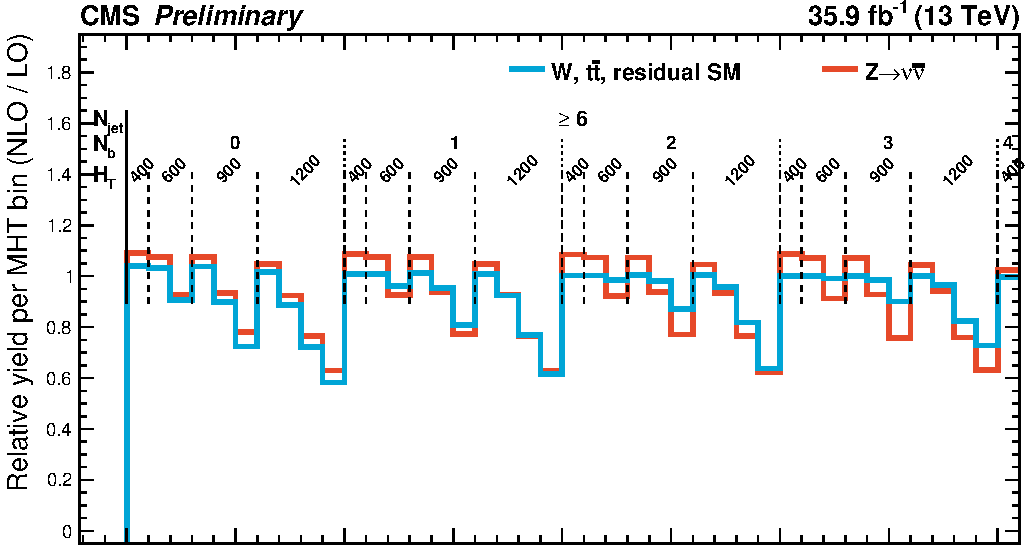
\includegraphics[width=0.48\textwidth]{figures/NLO/6+_jets_no-fit_NLO.pdf}
%  }\\
%  \caption{\label{fig:NLO_app} Size of the NLO corrections applied to data per MHT bin, in the signal region.
%	}
%\end{figure}
%

\clearpage
\subsection{Signal trigger efficiency}

\begin{figure}[!h]
  \centering
  \subfigure[Up variation versus (\njet,\nb) category and \scalht.]{
    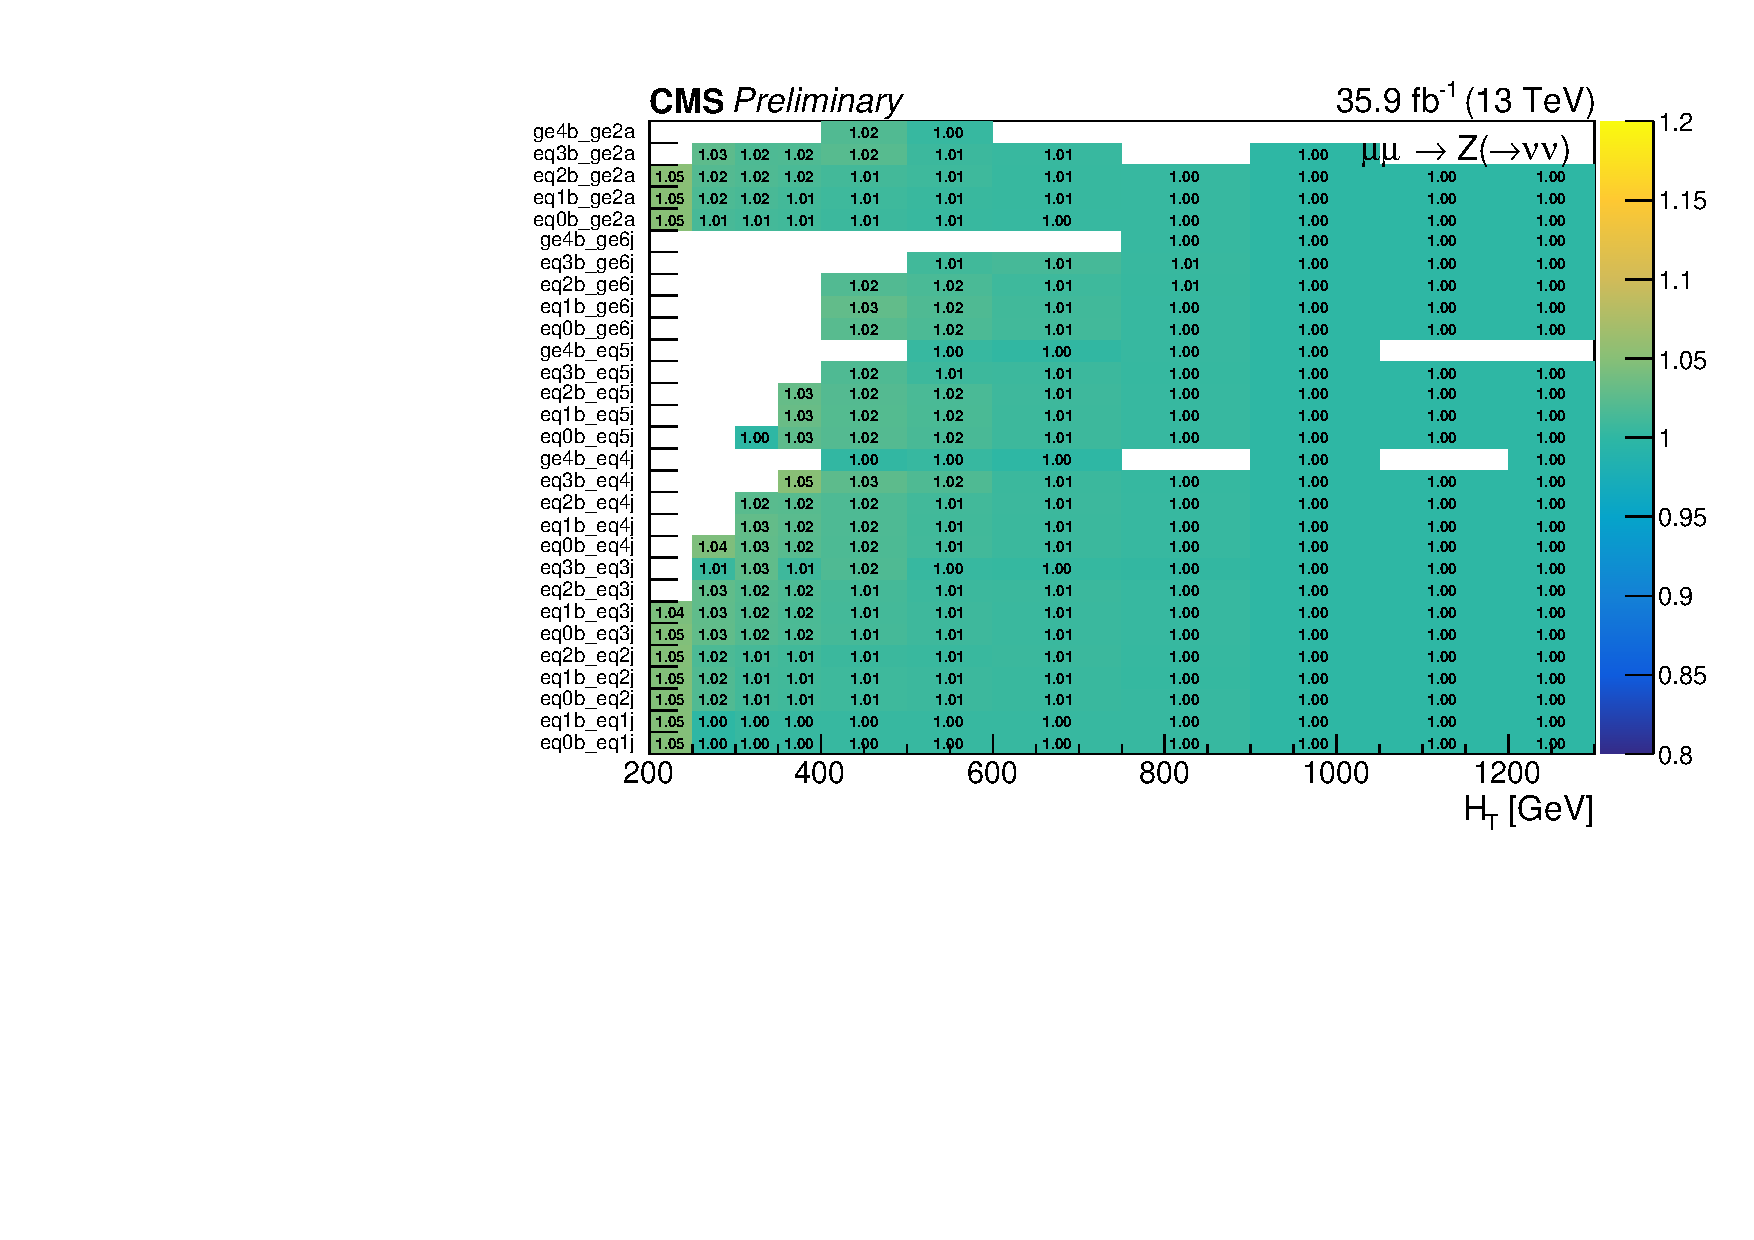
\includegraphics[width=0.5\textwidth]{figures/mcSystematics36p4fb/plots/tfratio_mumu_Zinv_2d_triggerWeightUp.pdf}
  } ~
  \subfigure[Down variation versus (\njet,\nb) category and \scalht.]{
    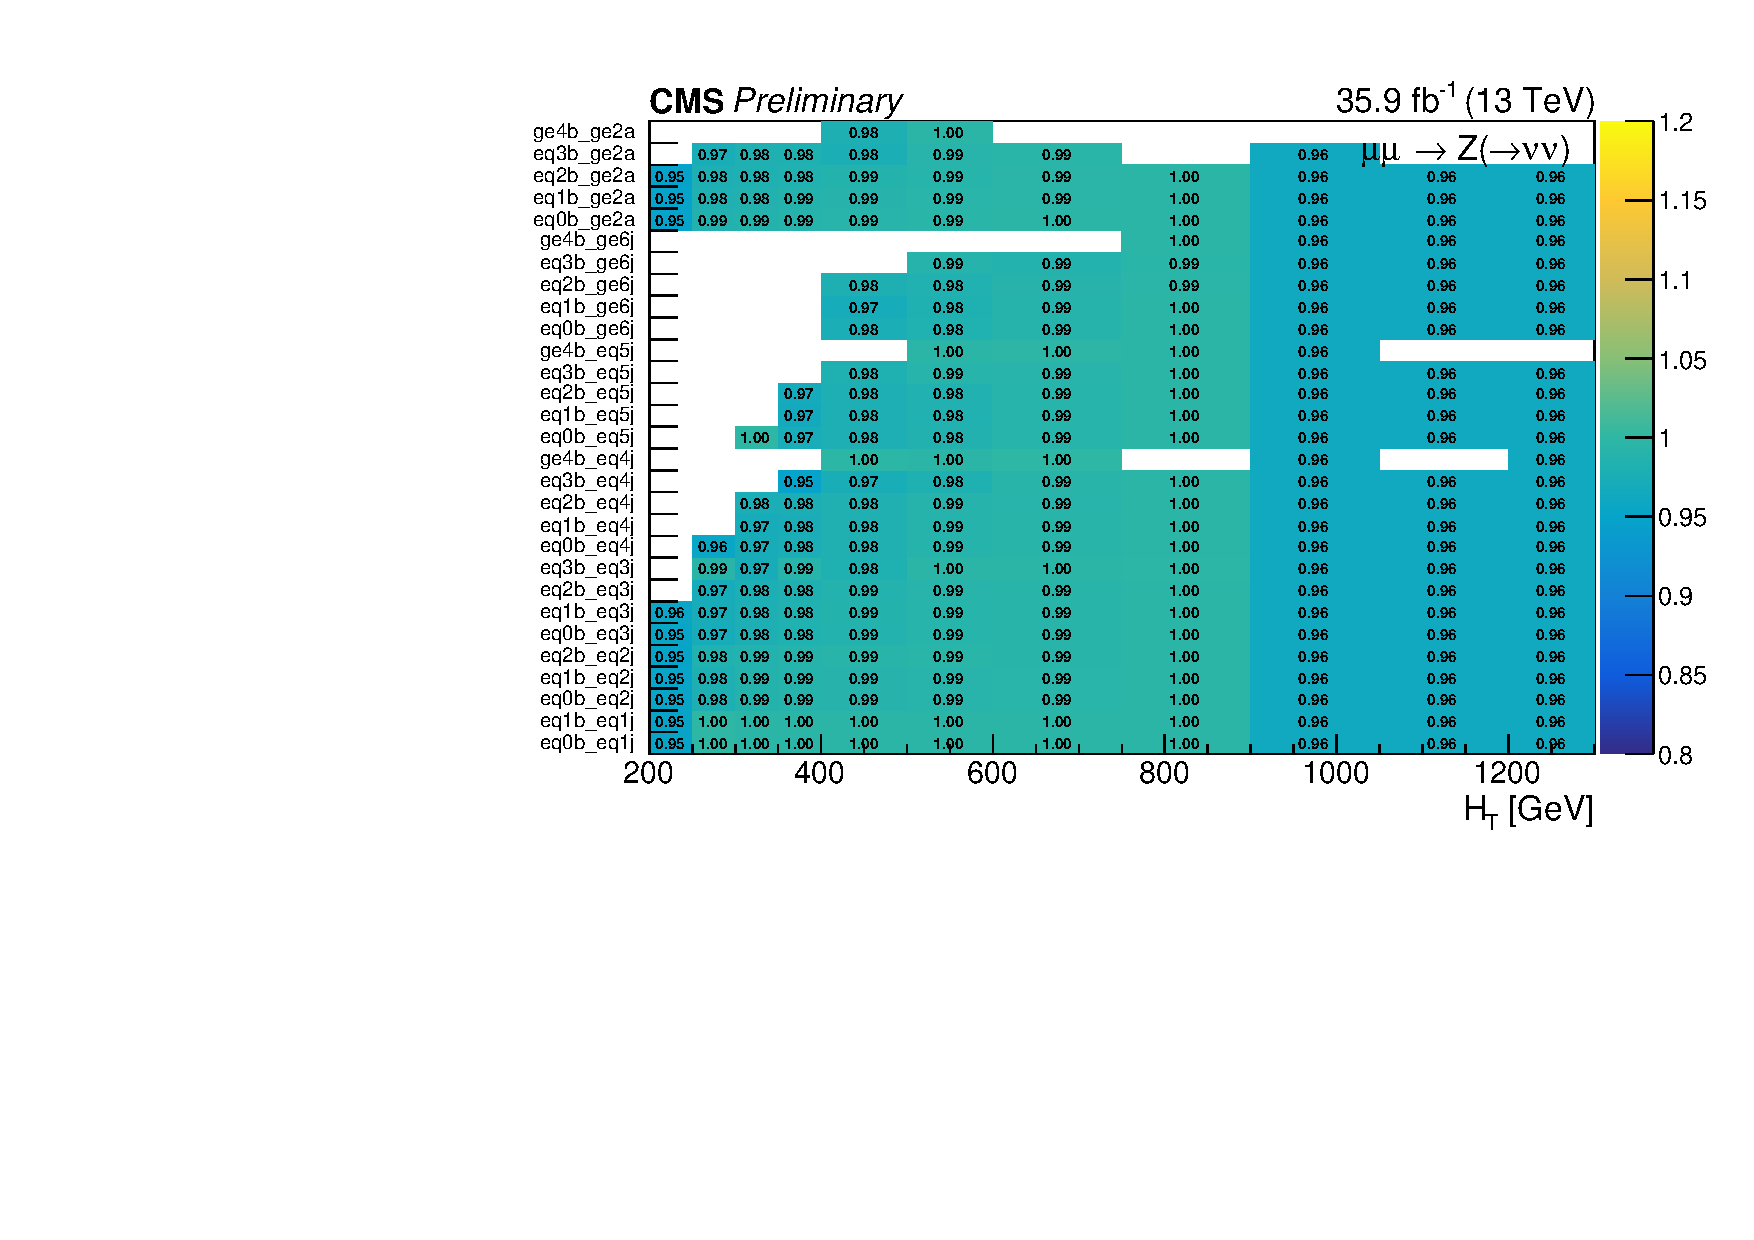
\includegraphics[width=0.5\textwidth]{figures/mcSystematics36p4fb/plots/tfratio_mumu_Zinv_2d_triggerWeightDown.pdf}
  }\\
  \subfigure[Up/down variations versus \njet.]{
    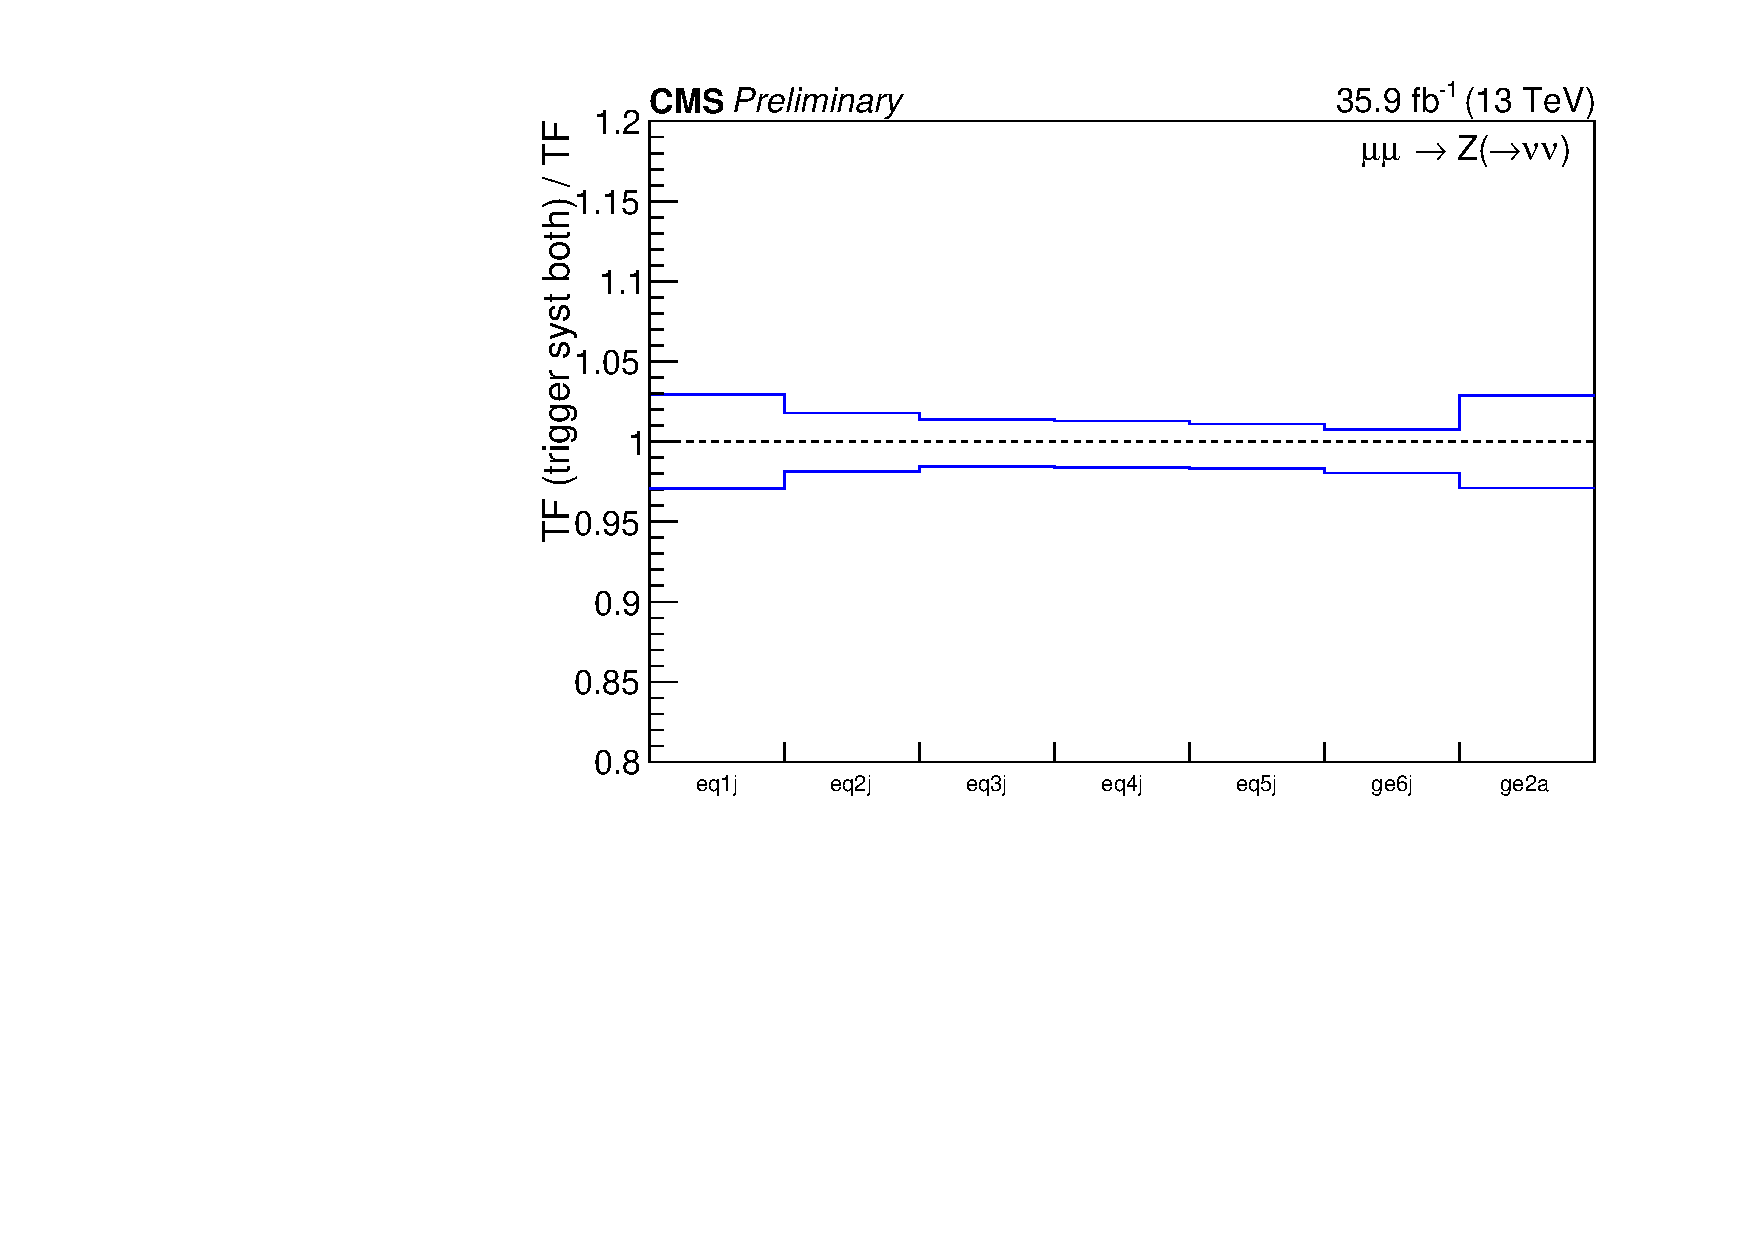
\includegraphics[width=0.5\textwidth]{figures/mcSystematics36p4fb/plots/tfratio_mumu_Zinv_njet_triggerWeightUp.pdf}
  } ~
  \subfigure[Up/down variations versus \scalht.]{
    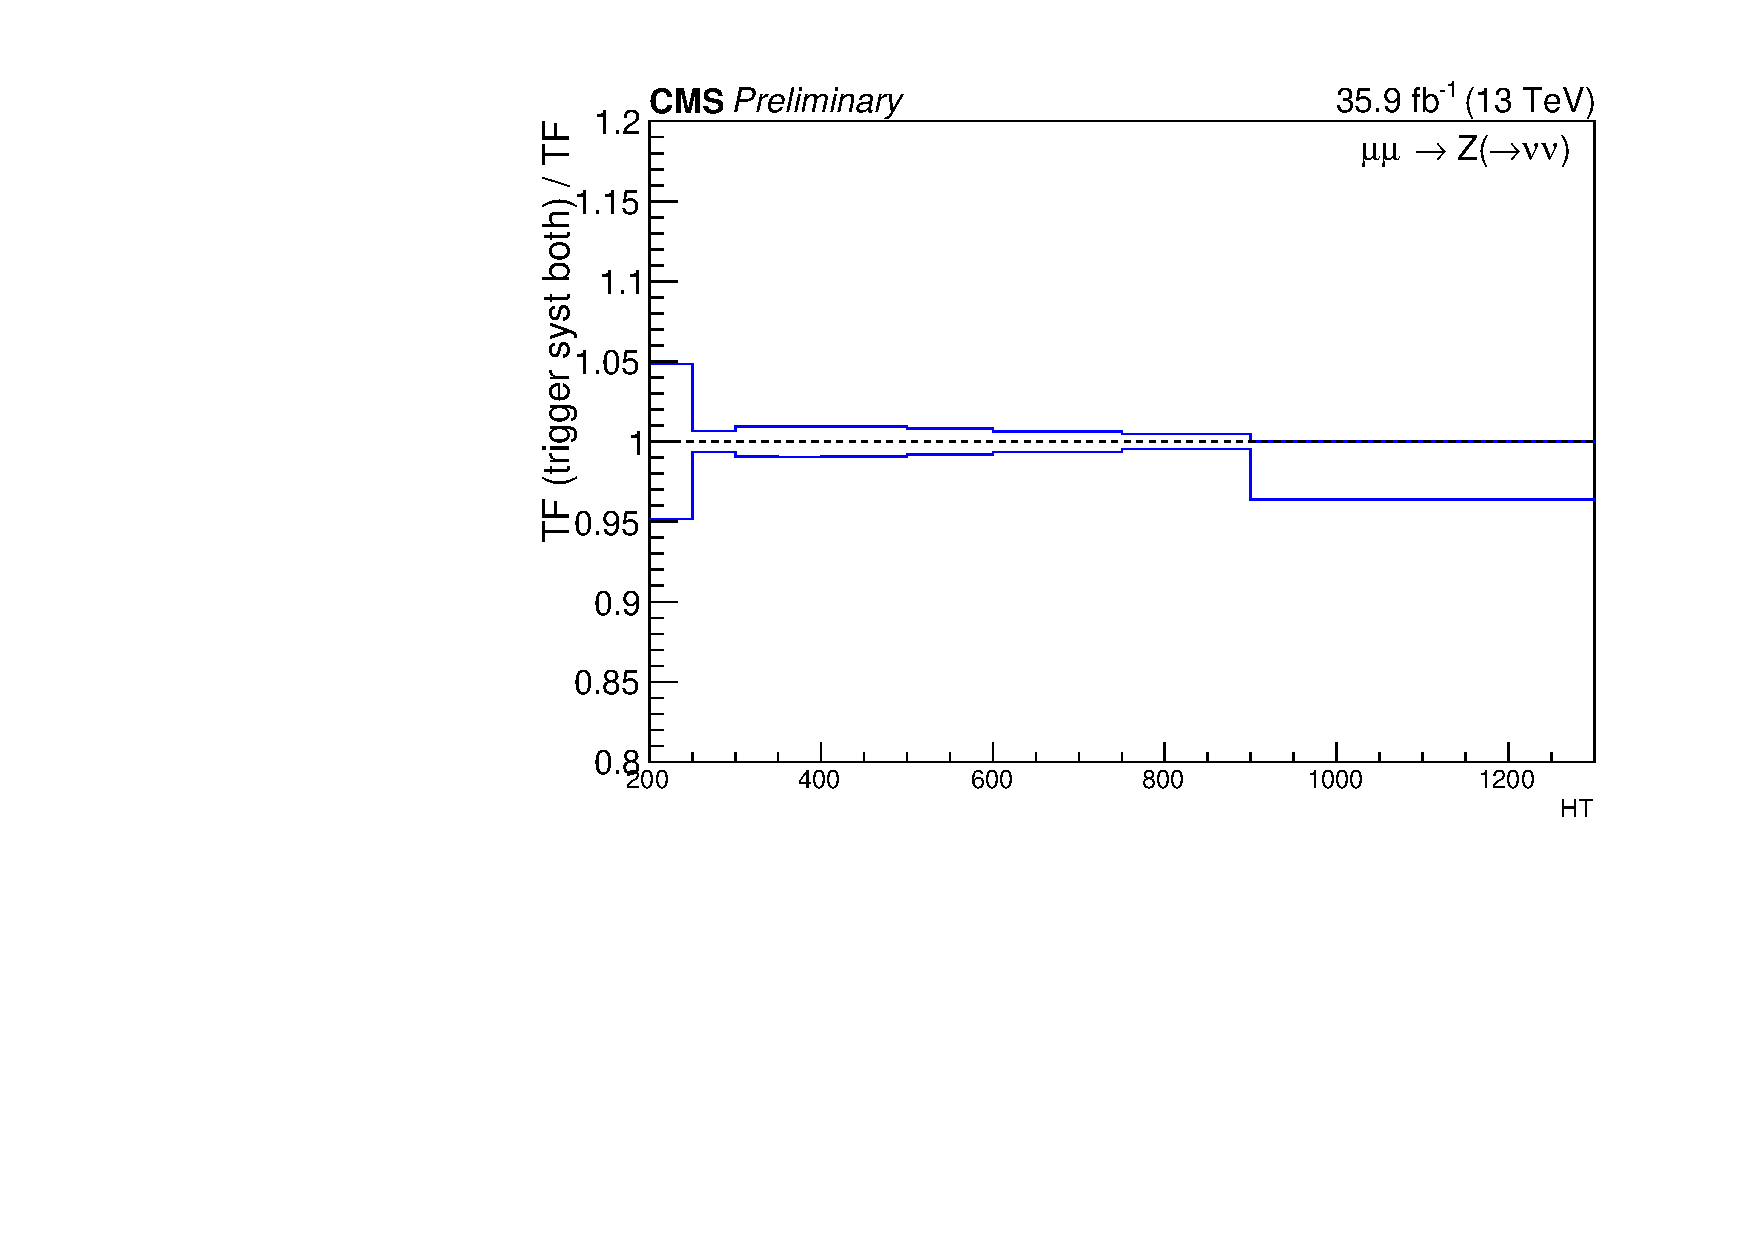
\includegraphics[width=0.5\textwidth]{figures/mcSystematics36p4fb/plots/tfratio_mumu_Zinv_ht_triggerWeightUp.pdf}
  } \\
  \subfigure[Up/down variations versus \nb.]{
    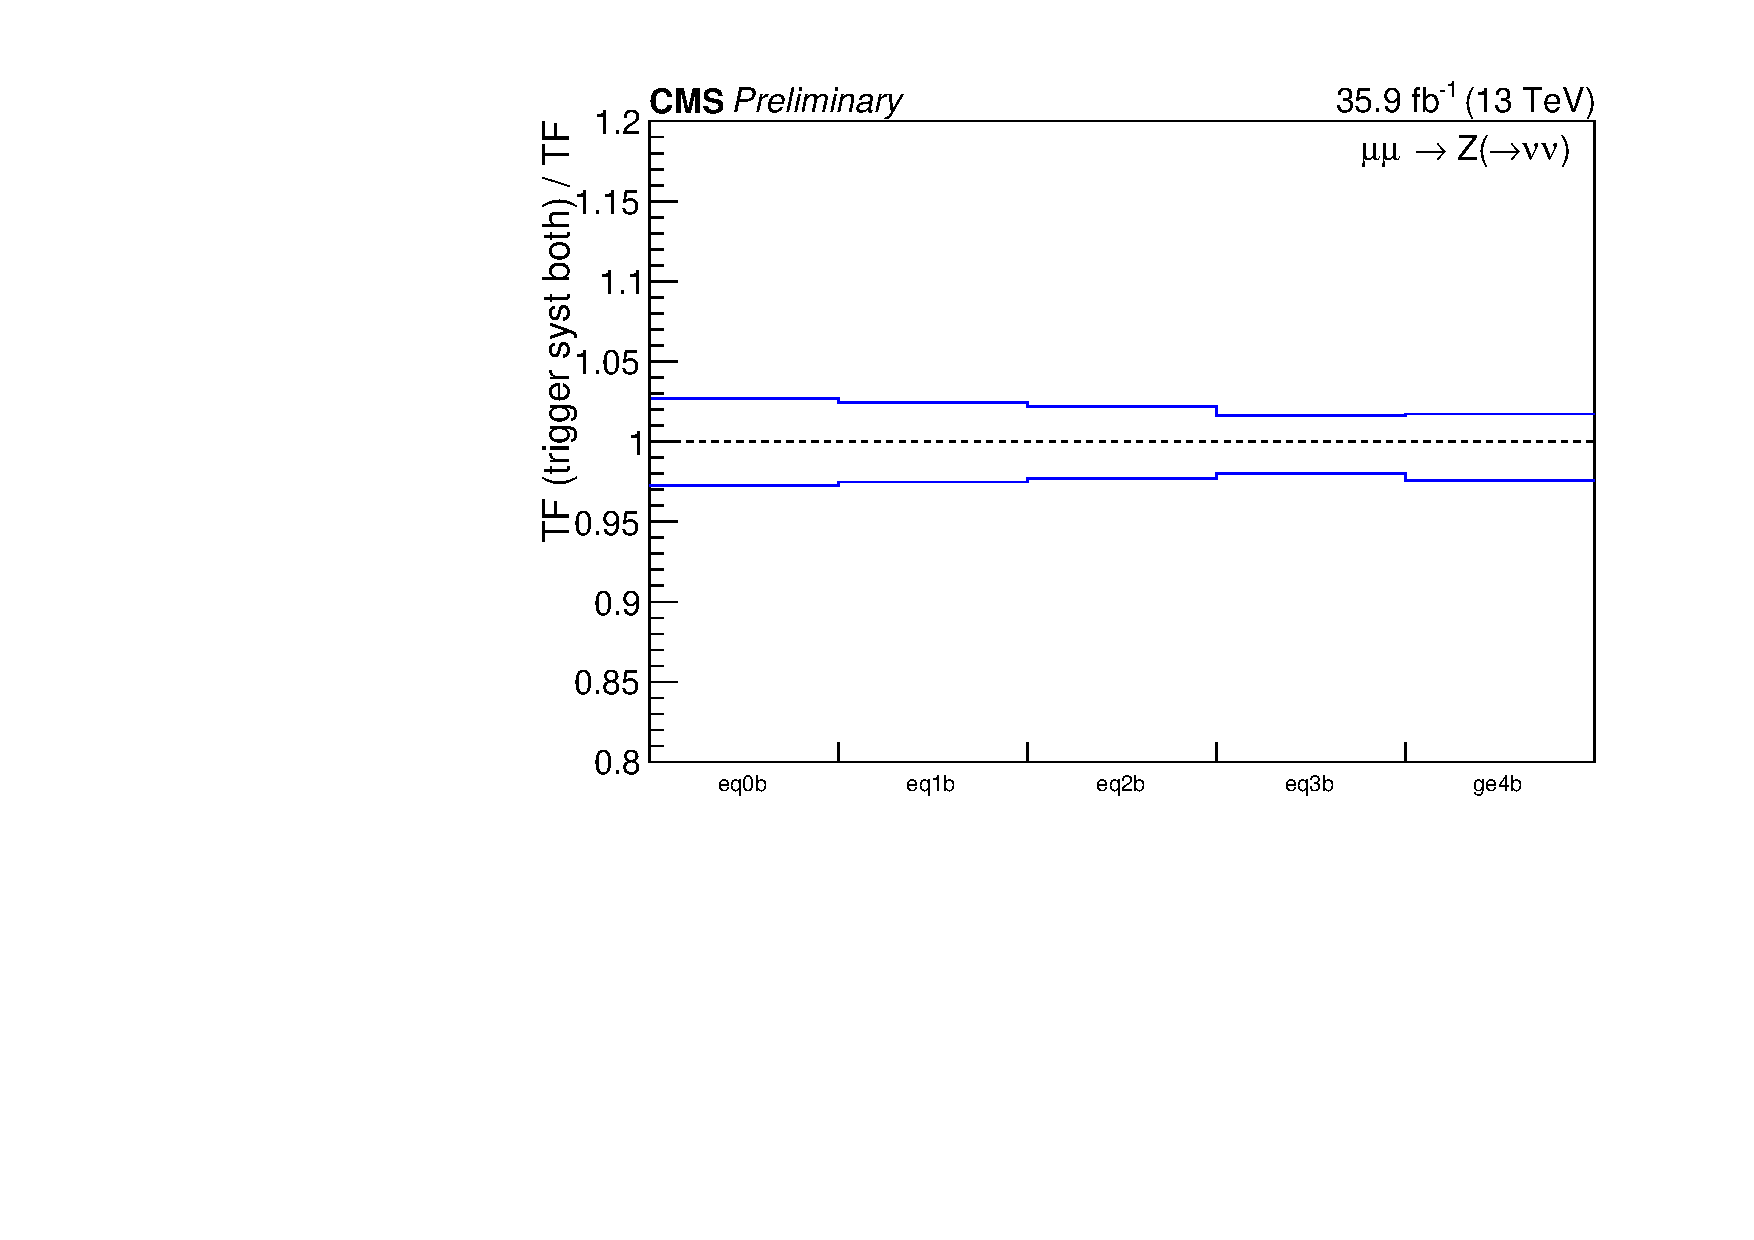
\includegraphics[width=0.5\textwidth]{figures/mcSystematics36p4fb/plots/tfratio_mumu_Zinv_bjet_triggerWeightUp.pdf}
  } ~
  \subfigure[Up/down variations versus \mht.]{
    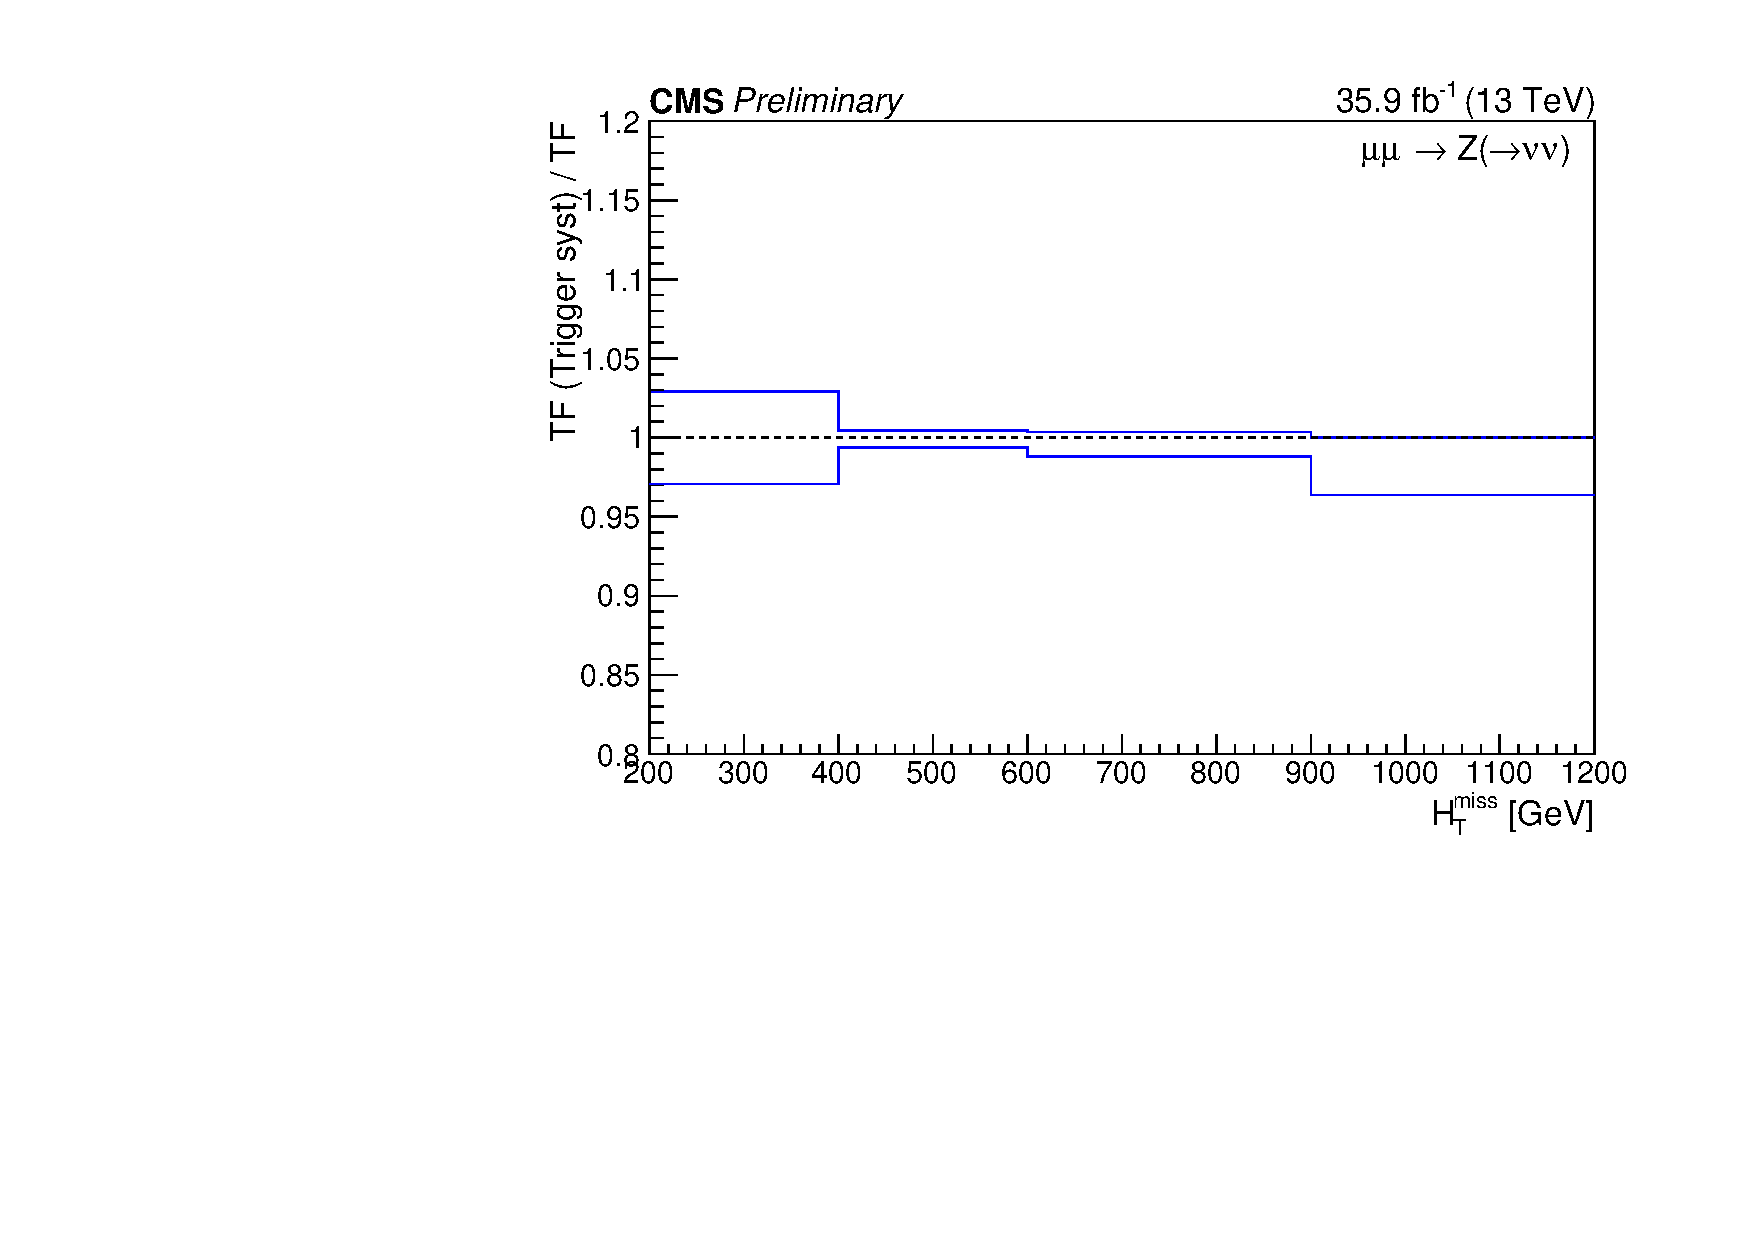
\includegraphics[width=0.5\textwidth]{figures/mcSystematics36p4fb/plots/tfratio_mumu_Zinv_mht_triggerWeightUp.pdf}
  } \\
  \caption{\label{fig:tfSyst_trigger_mmZinv} The relative change in the
    ``$\mmj \rightarrow \znunu\ + \textrm{jets}$'' transfer factors from
    simulation due to $\pm1\sigma$ uncertainties in the signal trigger
    efficiencies.  }
\end{figure}

\clearpage
\subsection{Lepton trigger / identification / isolation efficiencies}

\begin{figure}[!h]
  \centering
  \subfigure[Up variation versus (\njet,\nb) category and \scalht.]{
    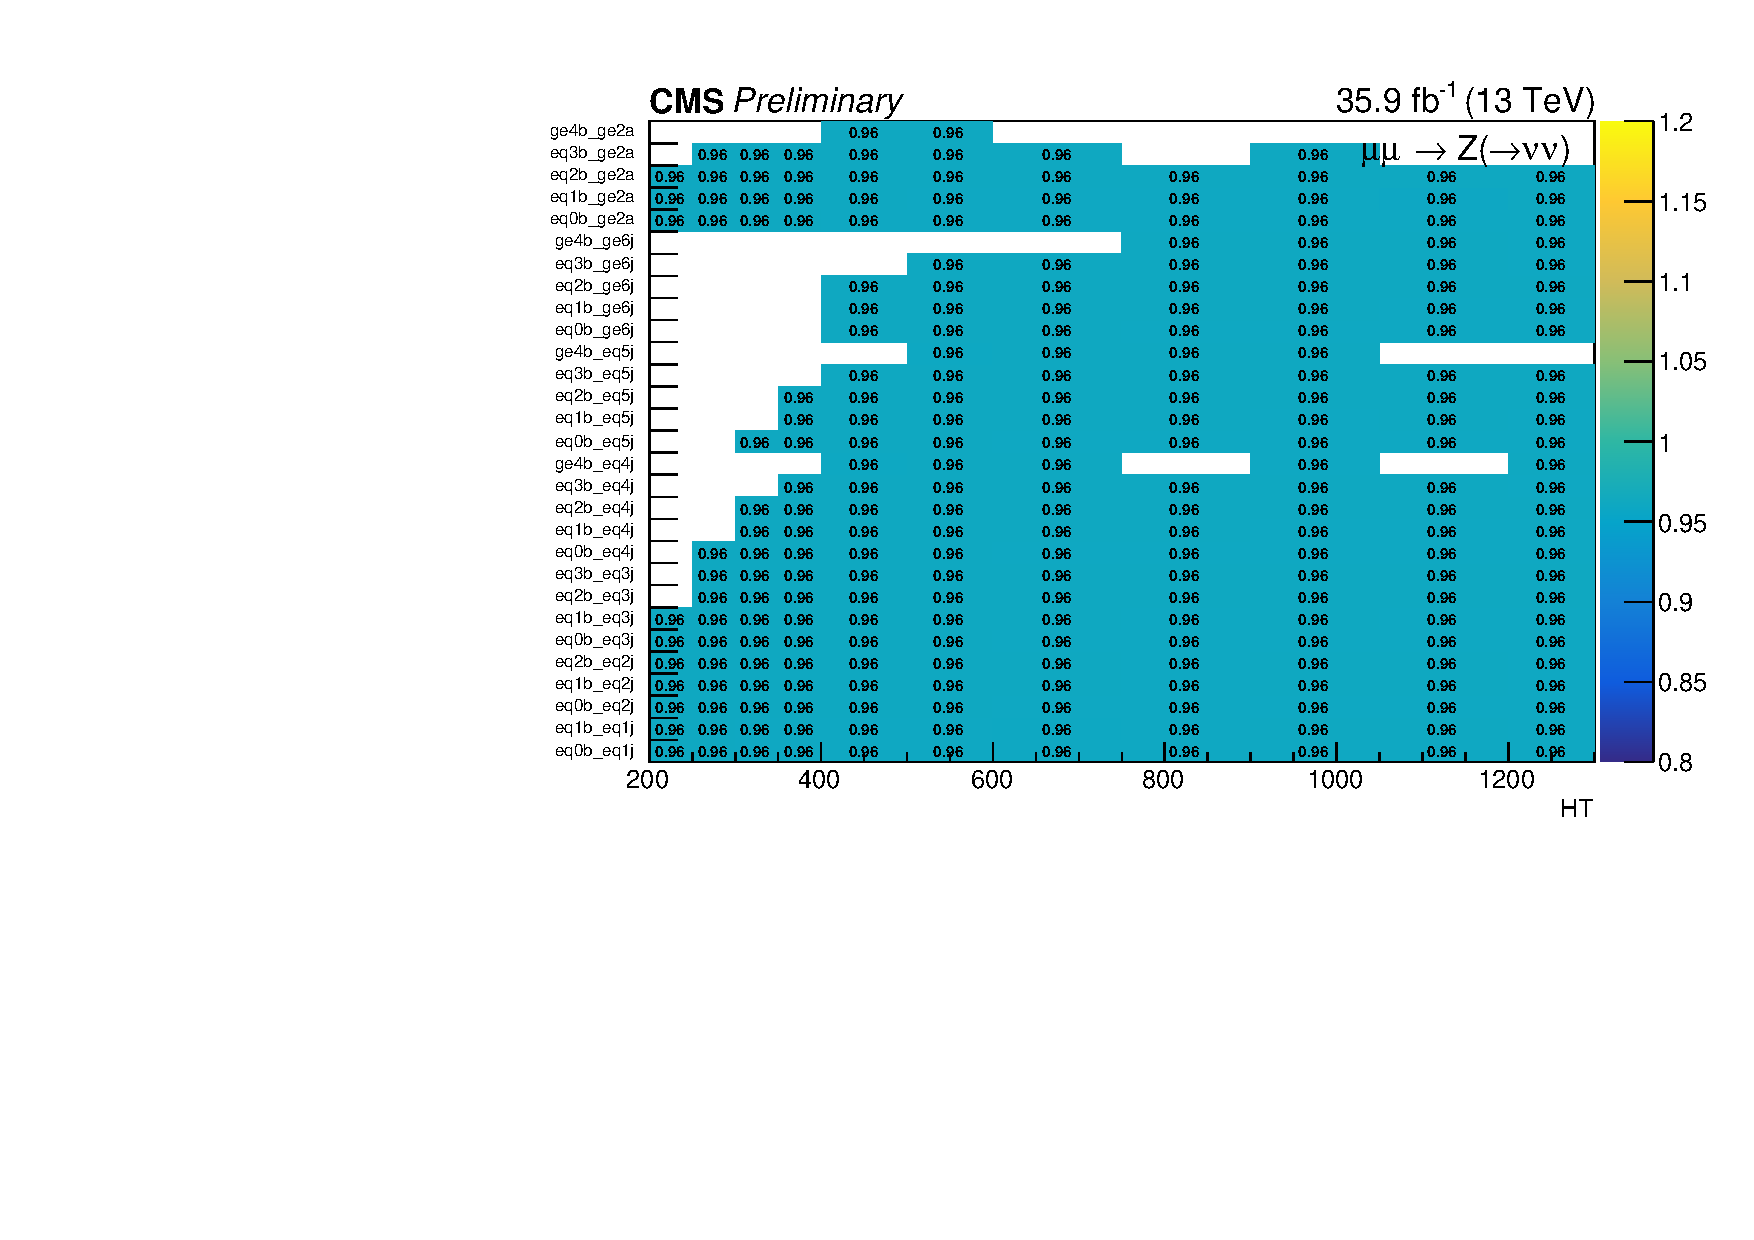
\includegraphics[width=0.5\textwidth]{figures/mcSystematics36p4fb/plots/tfratio_mumu_Zinv_2d_muonSfWeightUp.pdf}
  } ~
  \subfigure[Down variation versus (\njet,\nb) category and \scalht.]{
    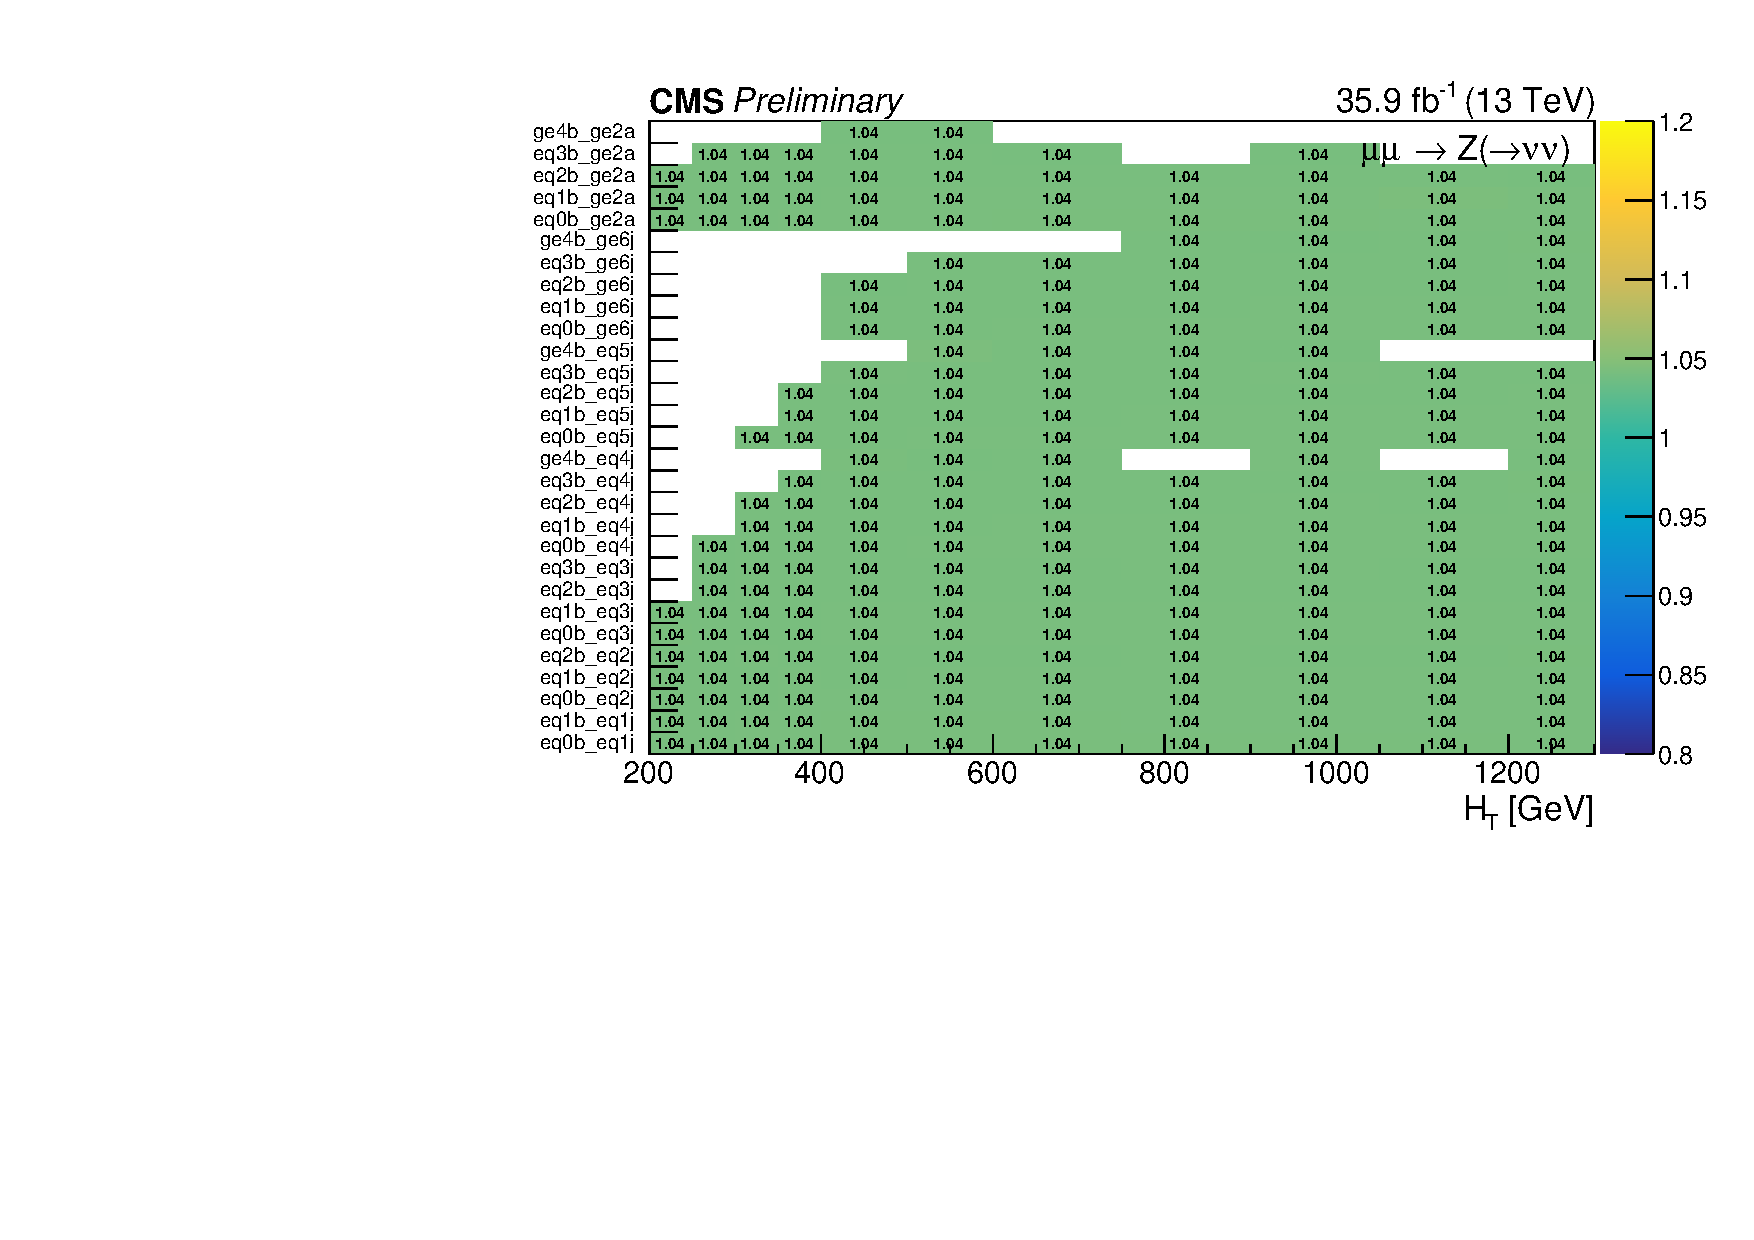
\includegraphics[width=0.5\textwidth]{figures/mcSystematics36p4fb/plots/tfratio_mumu_Zinv_2d_muonSfWeightDown.pdf}
  }\\
  \subfigure[Up/down variations versus \njet.]{
    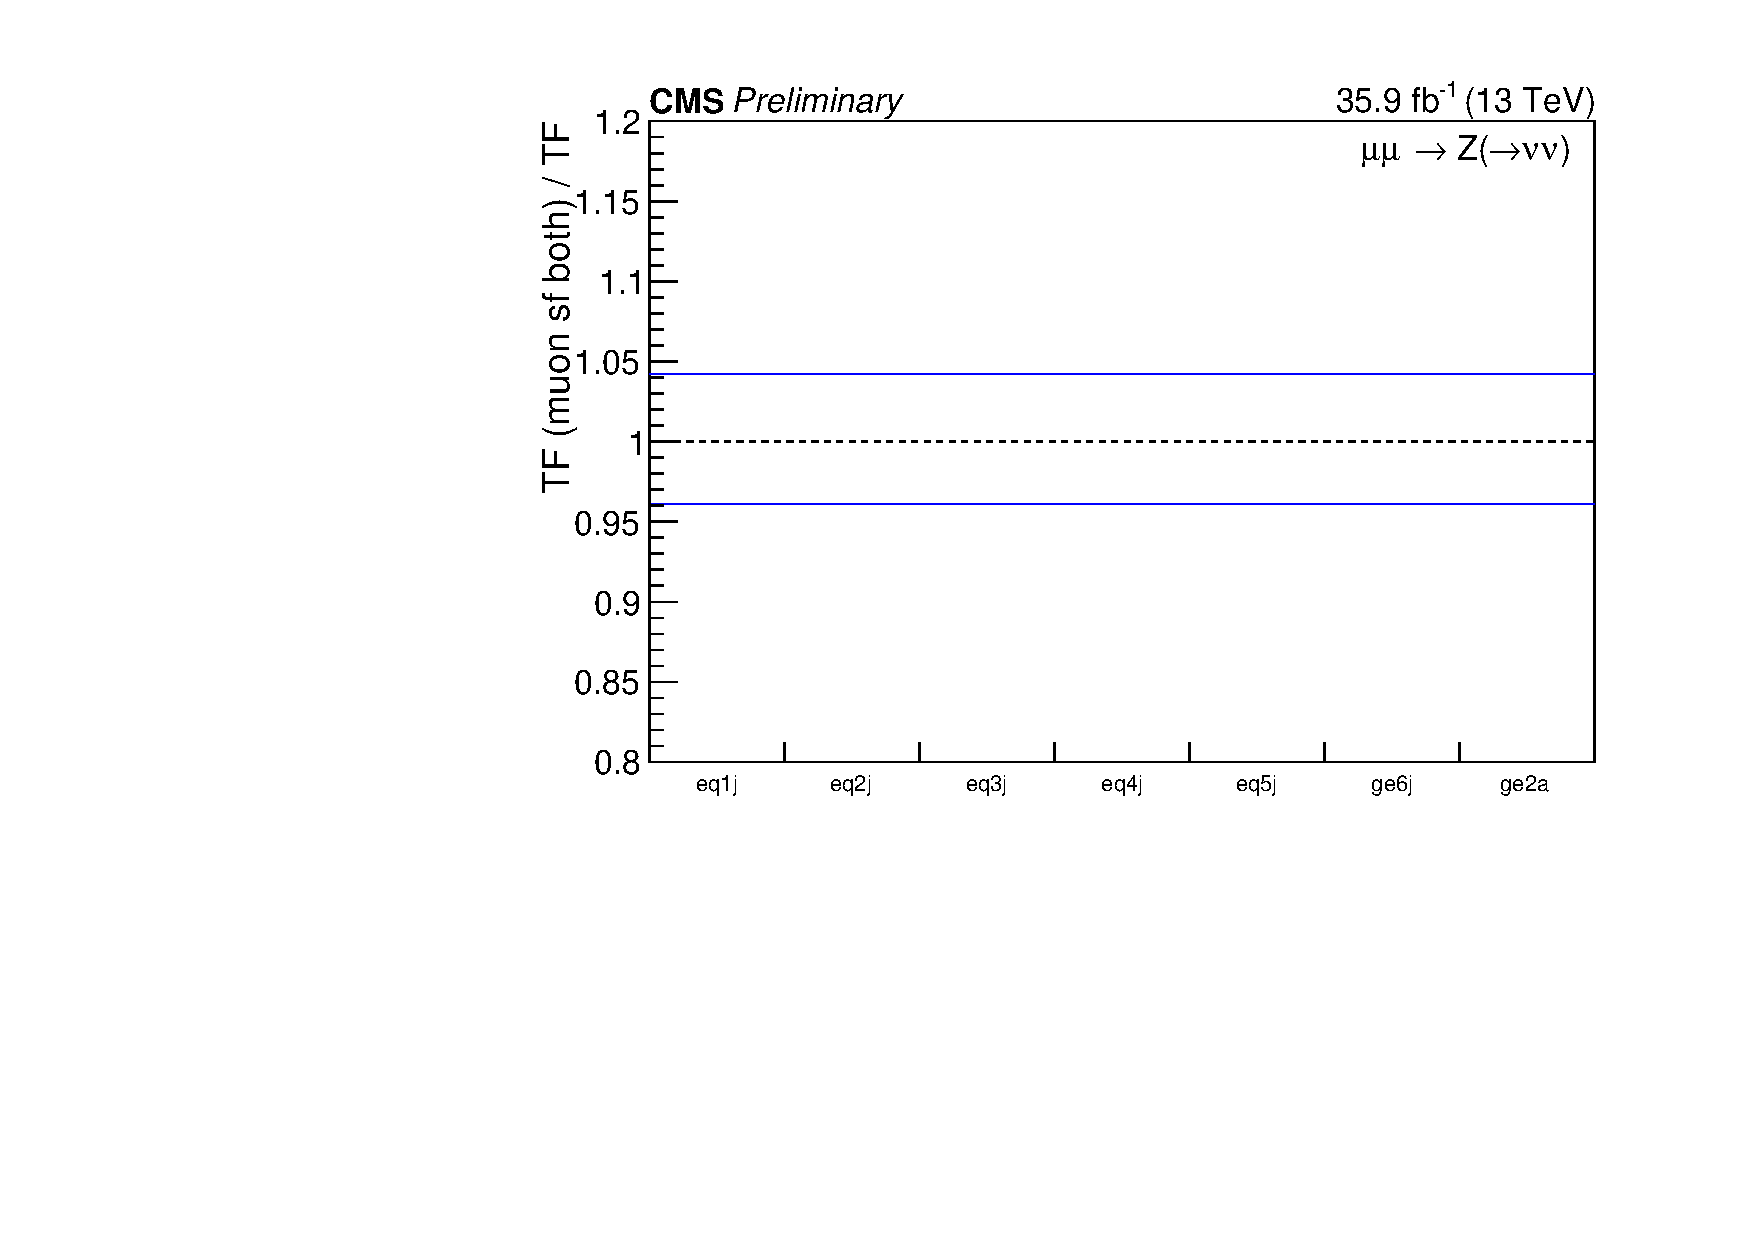
\includegraphics[width=0.5\textwidth]{figures/mcSystematics36p4fb/plots/tfratio_mumu_Zinv_njet_muonSfWeightUp.pdf}
  } ~
  \subfigure[Up/down variations versus \scalht.]{
    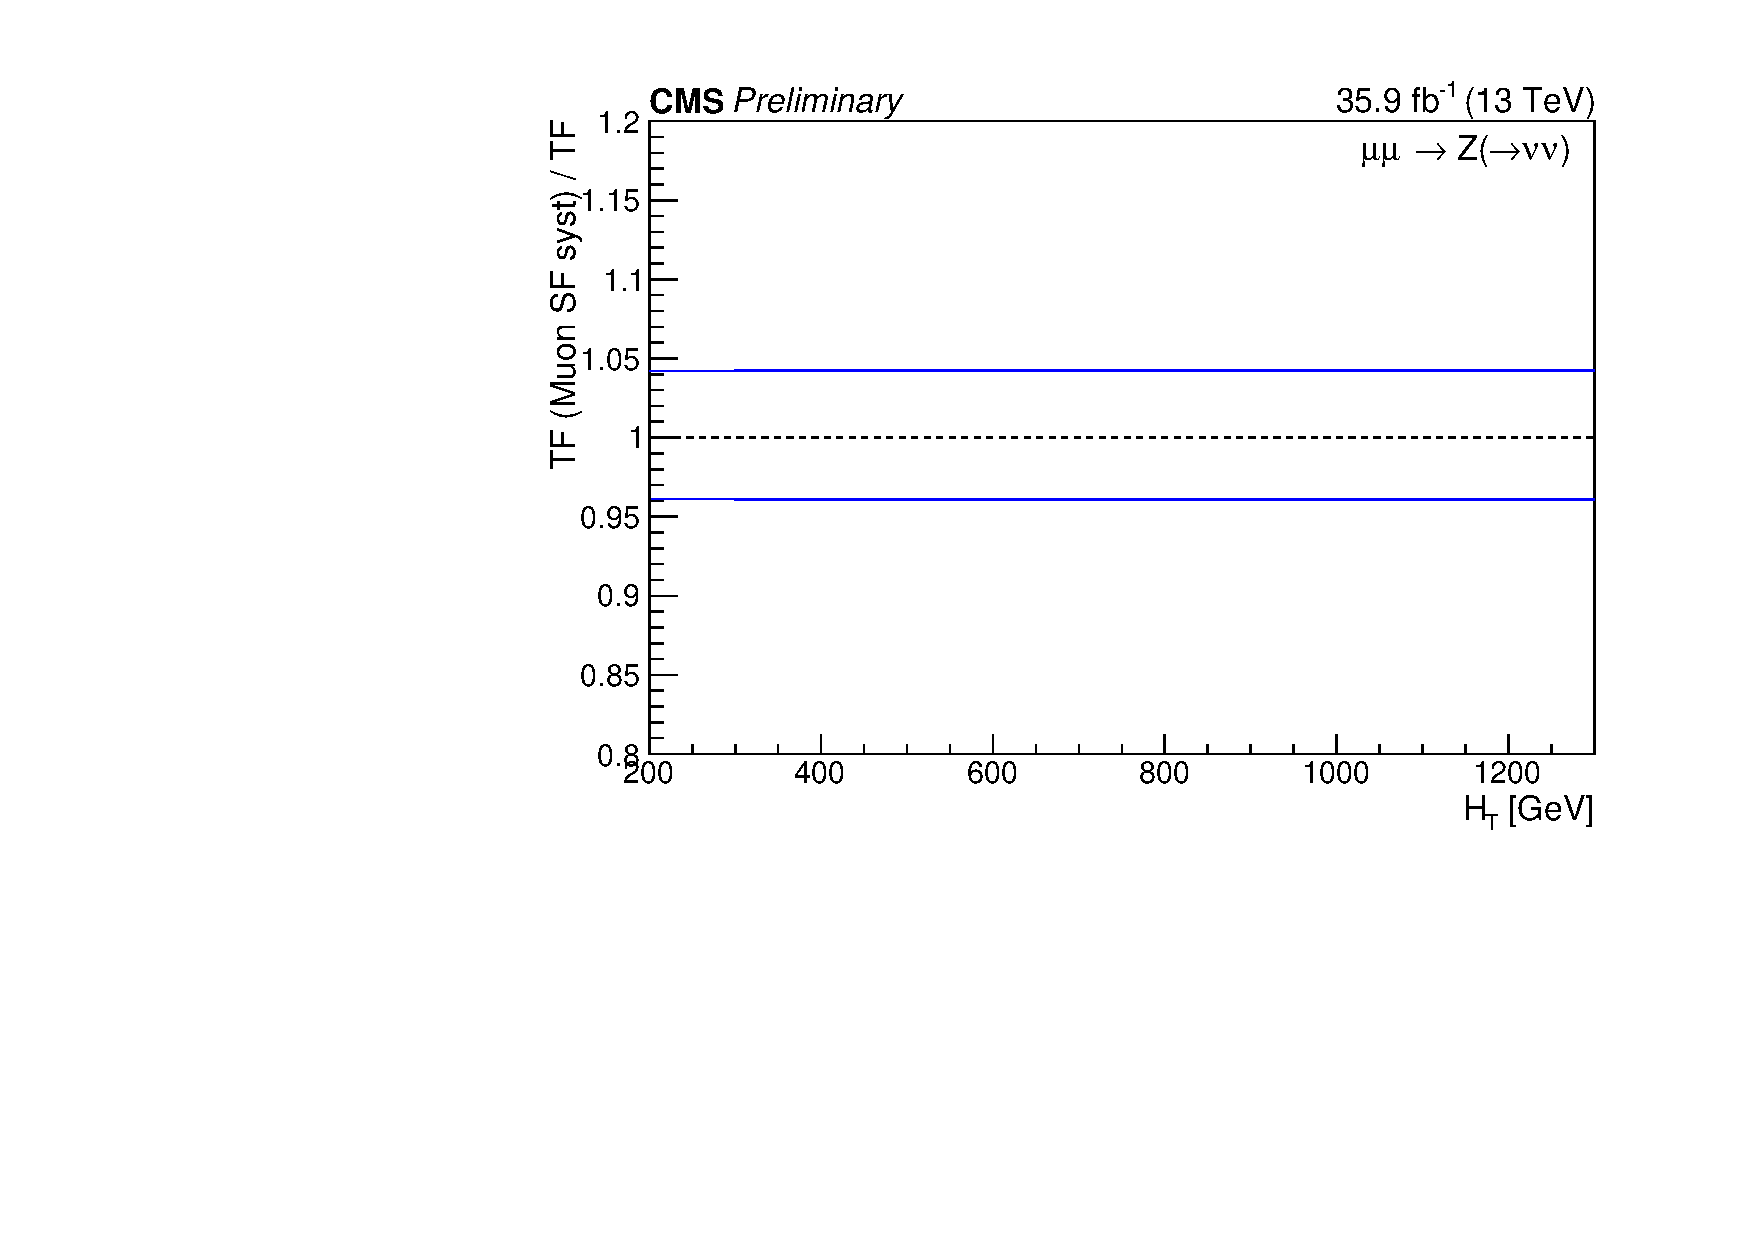
\includegraphics[width=0.5\textwidth]{figures/mcSystematics36p4fb/plots/tfratio_mumu_Zinv_ht_muonSfWeightUp.pdf}
  } \\
  \subfigure[Up/down variations versus \nb.]{
    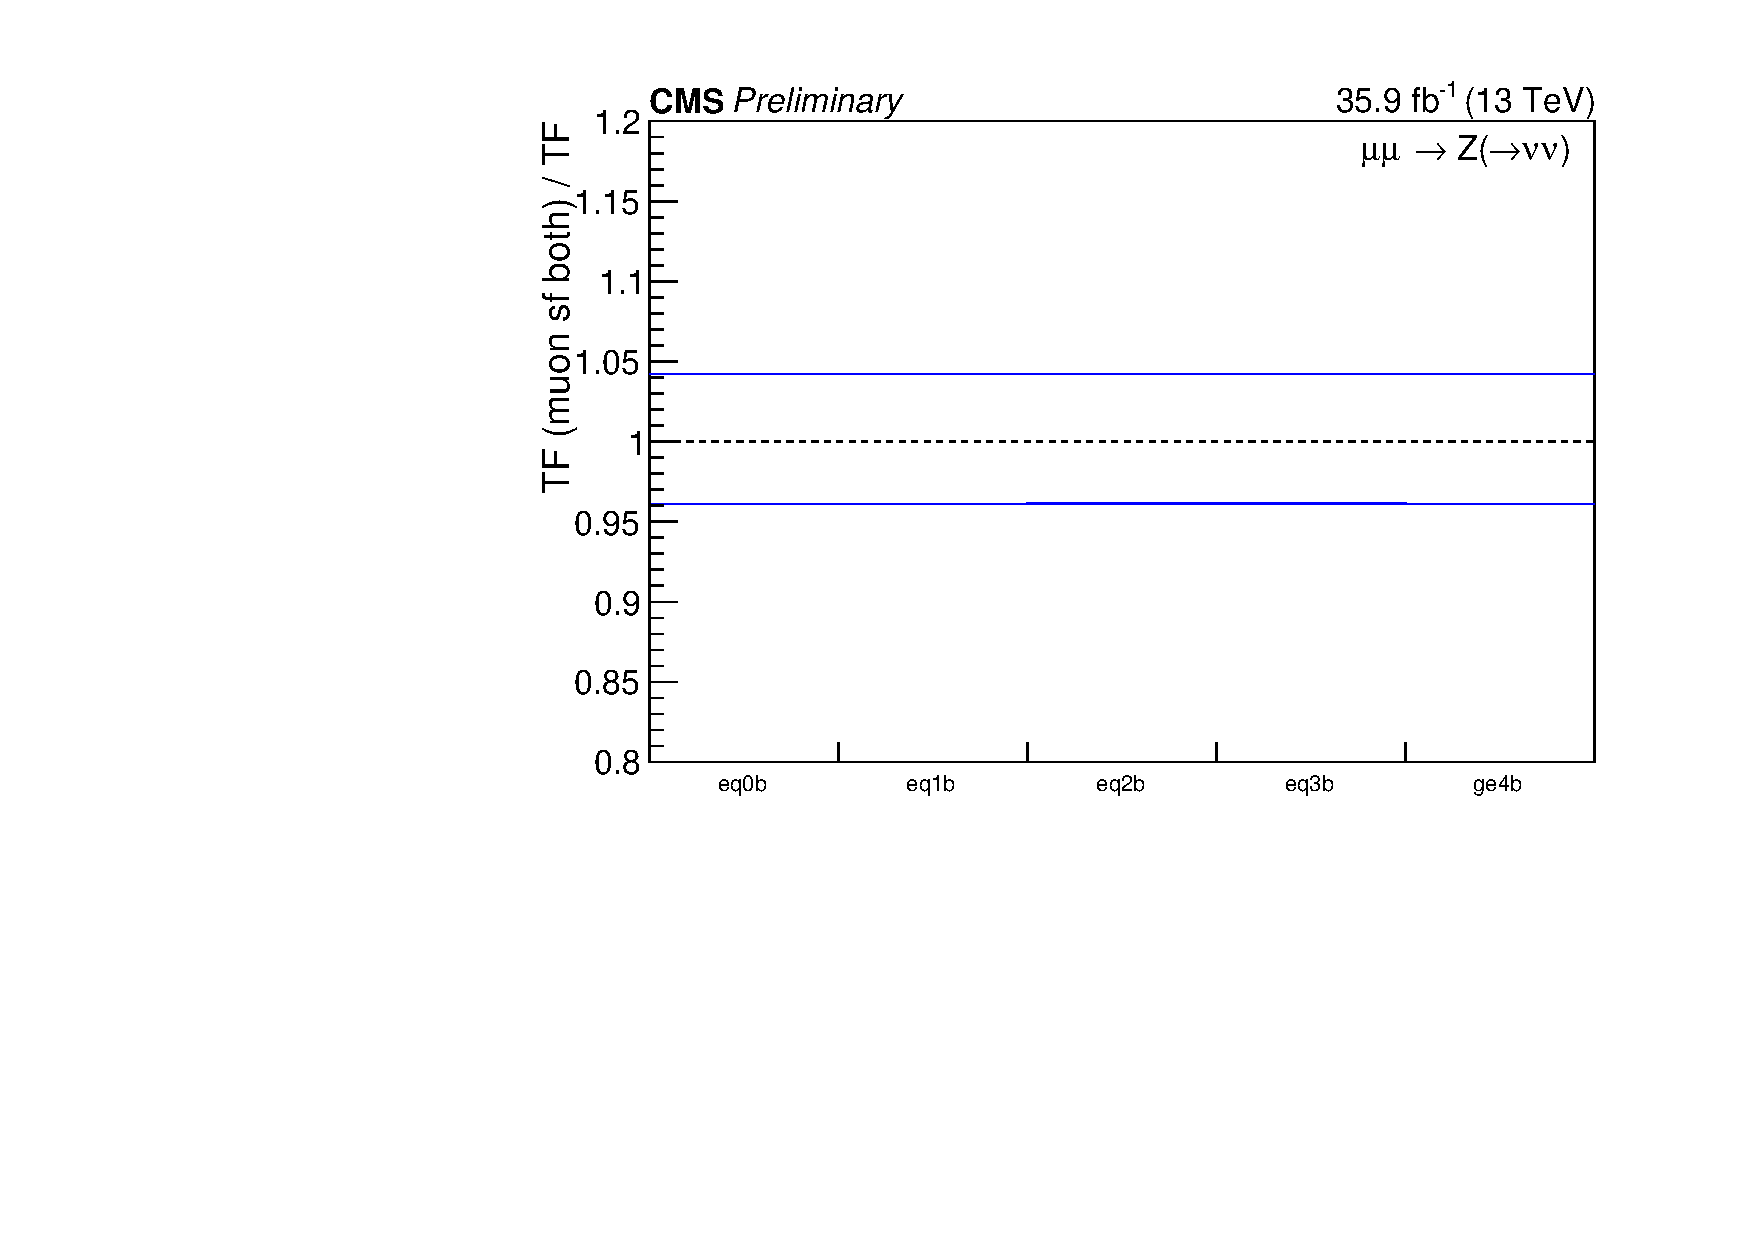
\includegraphics[width=0.5\textwidth]{figures/mcSystematics36p4fb/plots/tfratio_mumu_Zinv_bjet_muonSfWeightUp.pdf}
  } ~
  \subfigure[Up/down variations versus \mht.]{
    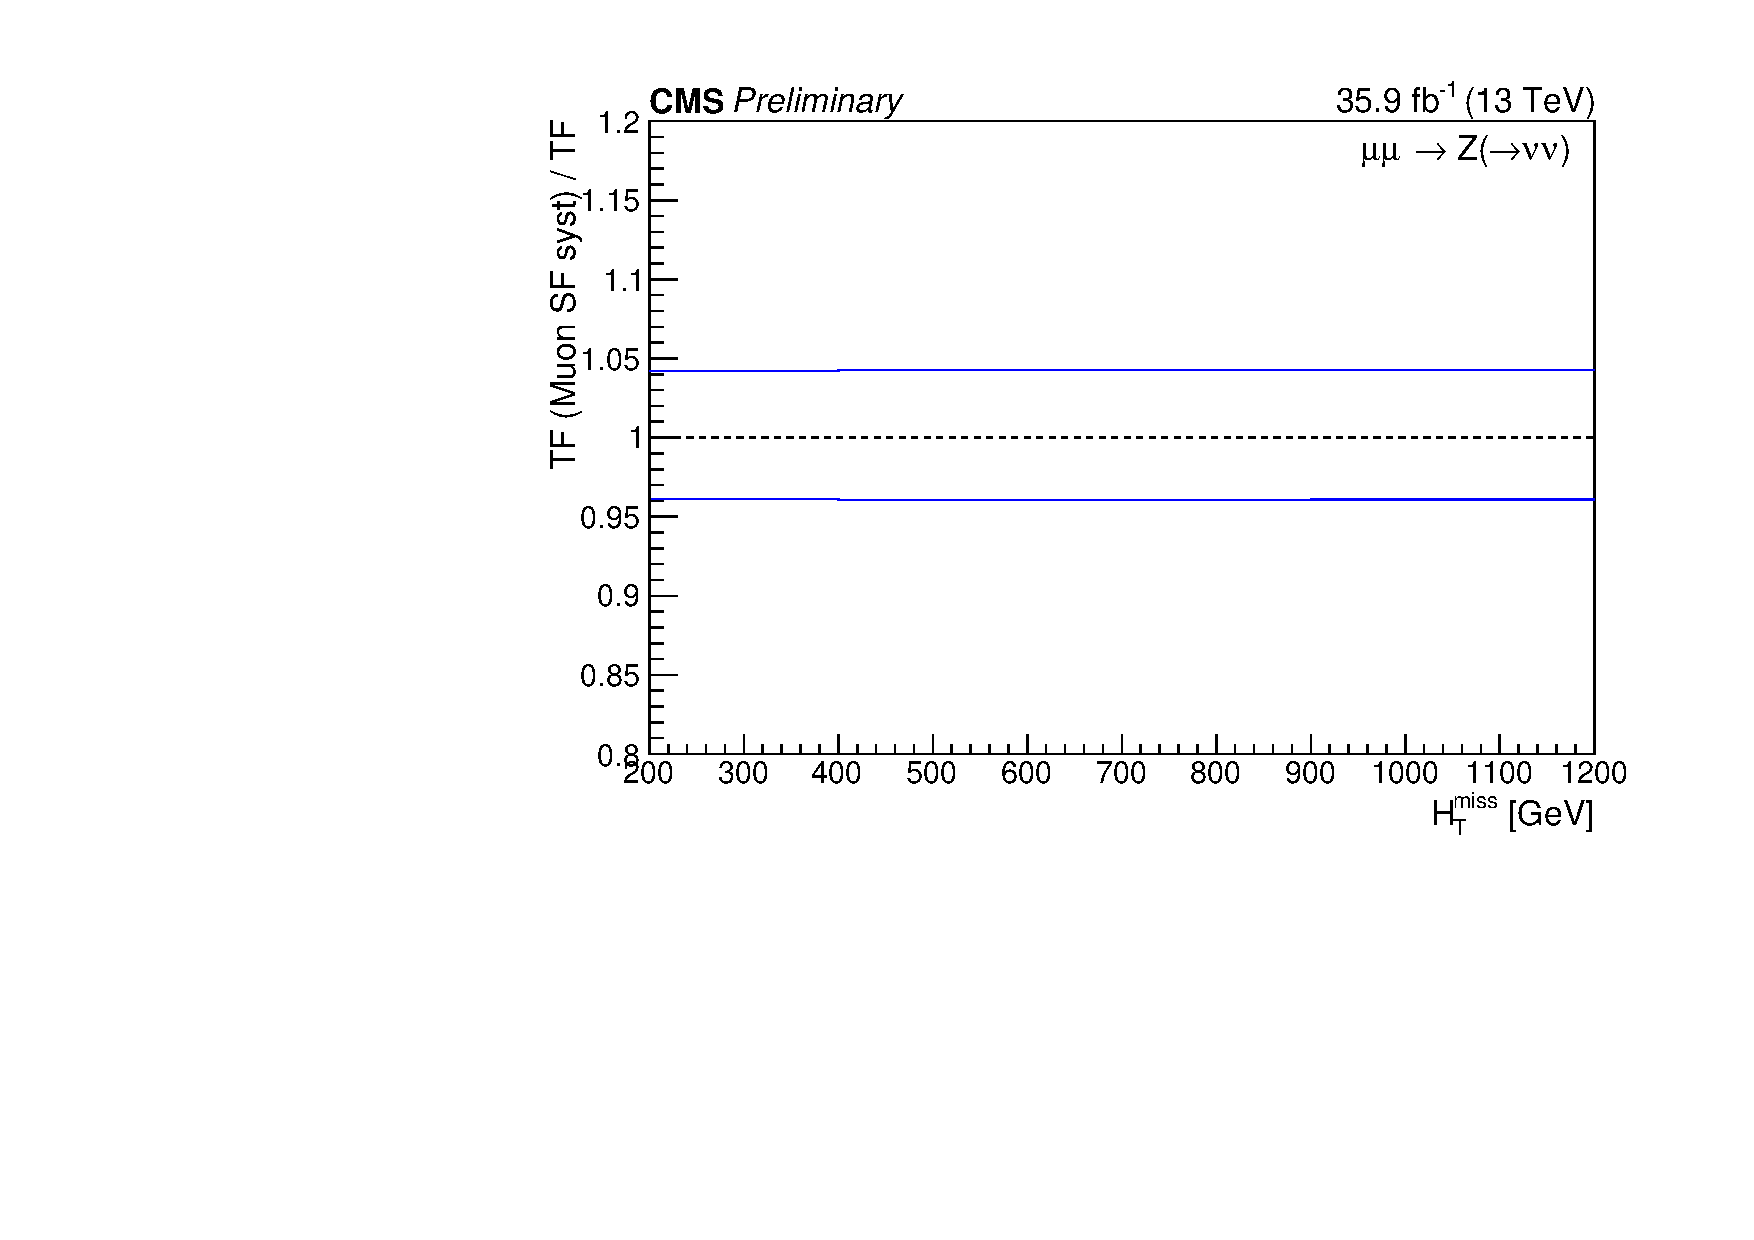
\includegraphics[width=0.5\textwidth]{figures/mcSystematics36p4fb/plots/tfratio_mumu_Zinv_mht_muonSfWeightUp.pdf}
  } \\
  \caption{\label{fig:tfSyst_muonsf_mmZinv} The relative change in the
    ``$\mmj \rightarrow \znunu\ + \textrm{jets}$'' transfer factors from
    simulation due to $\pm1\sigma$ uncertainties in efficiencies
    related to muon trigger, identification, and isolation.  }
\end{figure}

\clearpage
\subsection{Jet energy scale}

\begin{figure}[!h]
  \centering
  \subfigure[Up variation versus (\njet,\nb) category and \scalht.]{
    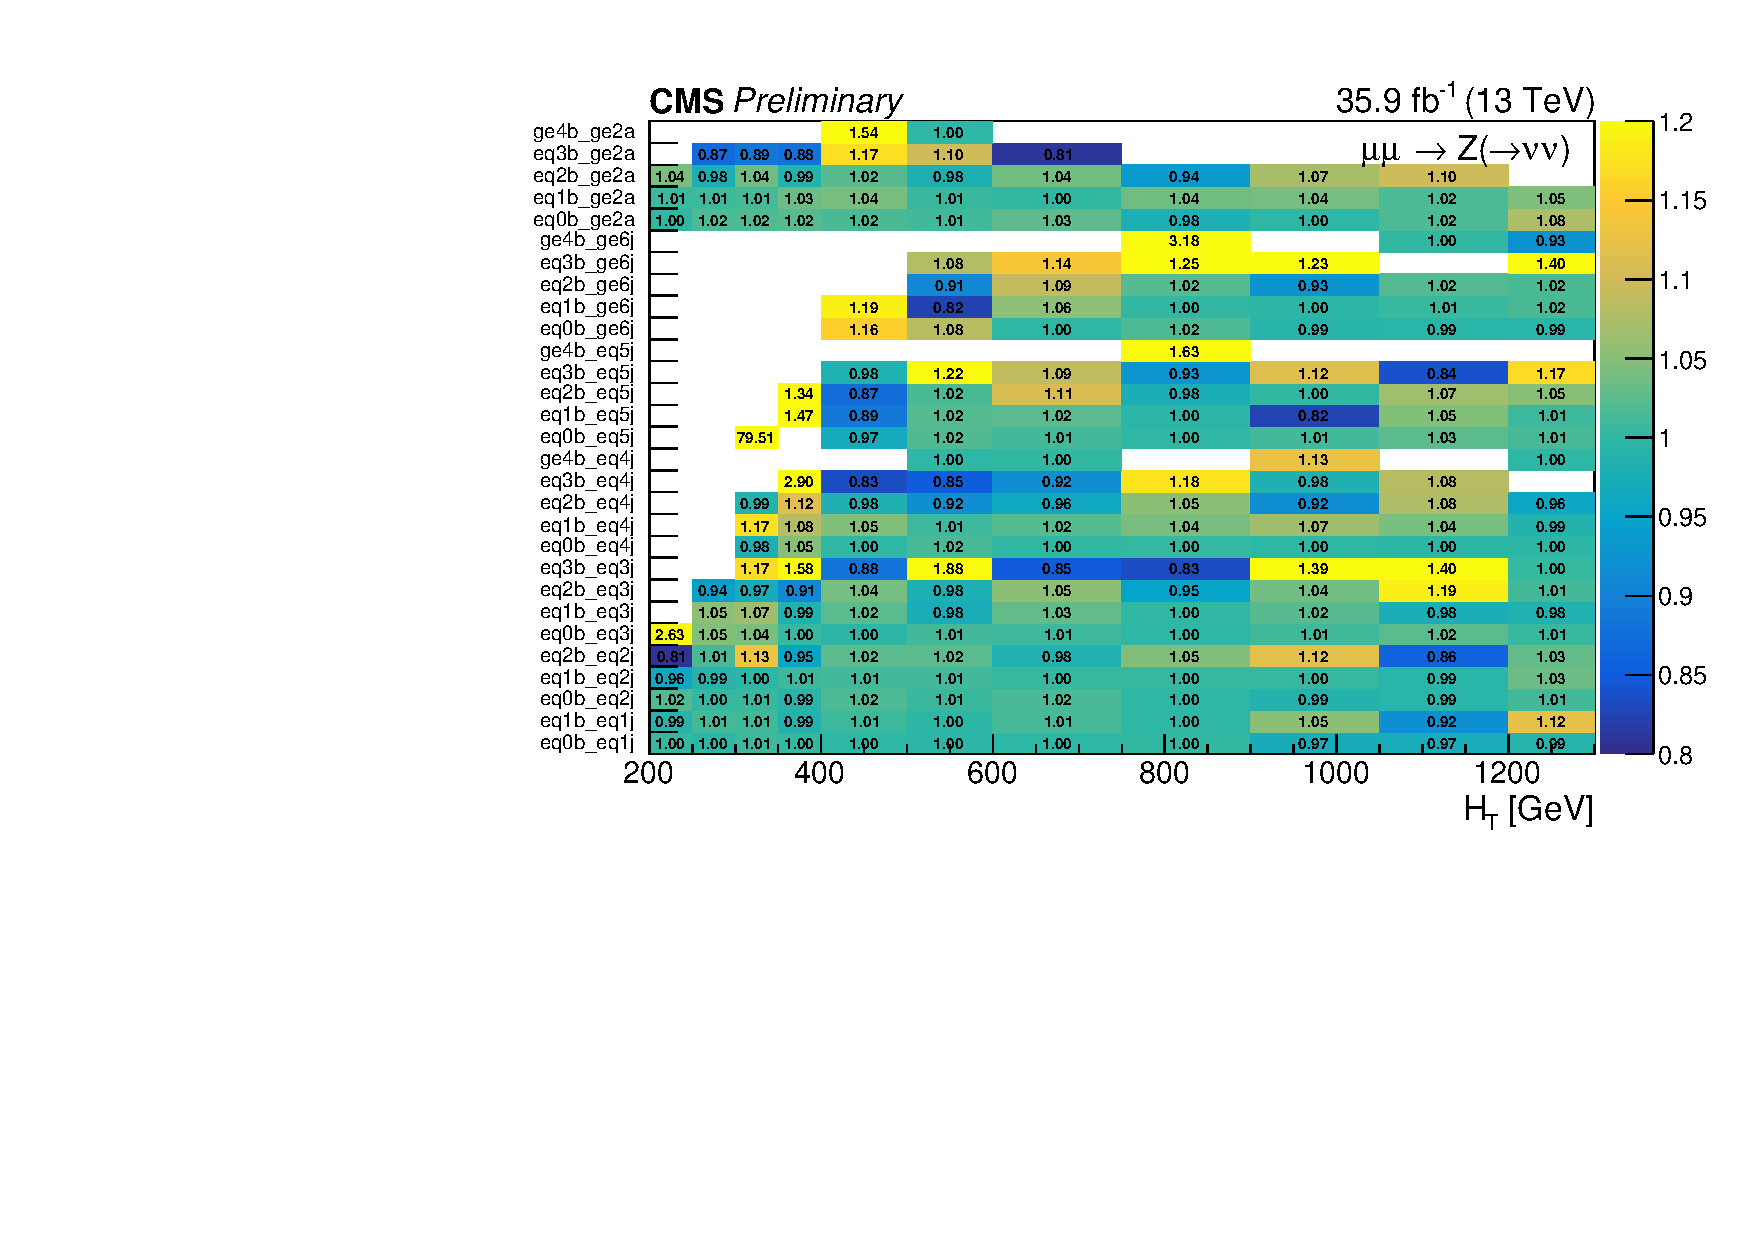
\includegraphics[width=0.5\textwidth]{figures/mcSystematics36p4fb/plots/tfratio_mumu_Zinv_2d_jecUp.pdf}
  } ~
  \subfigure[Down variation versus (\njet,\nb) category and \scalht.]{
    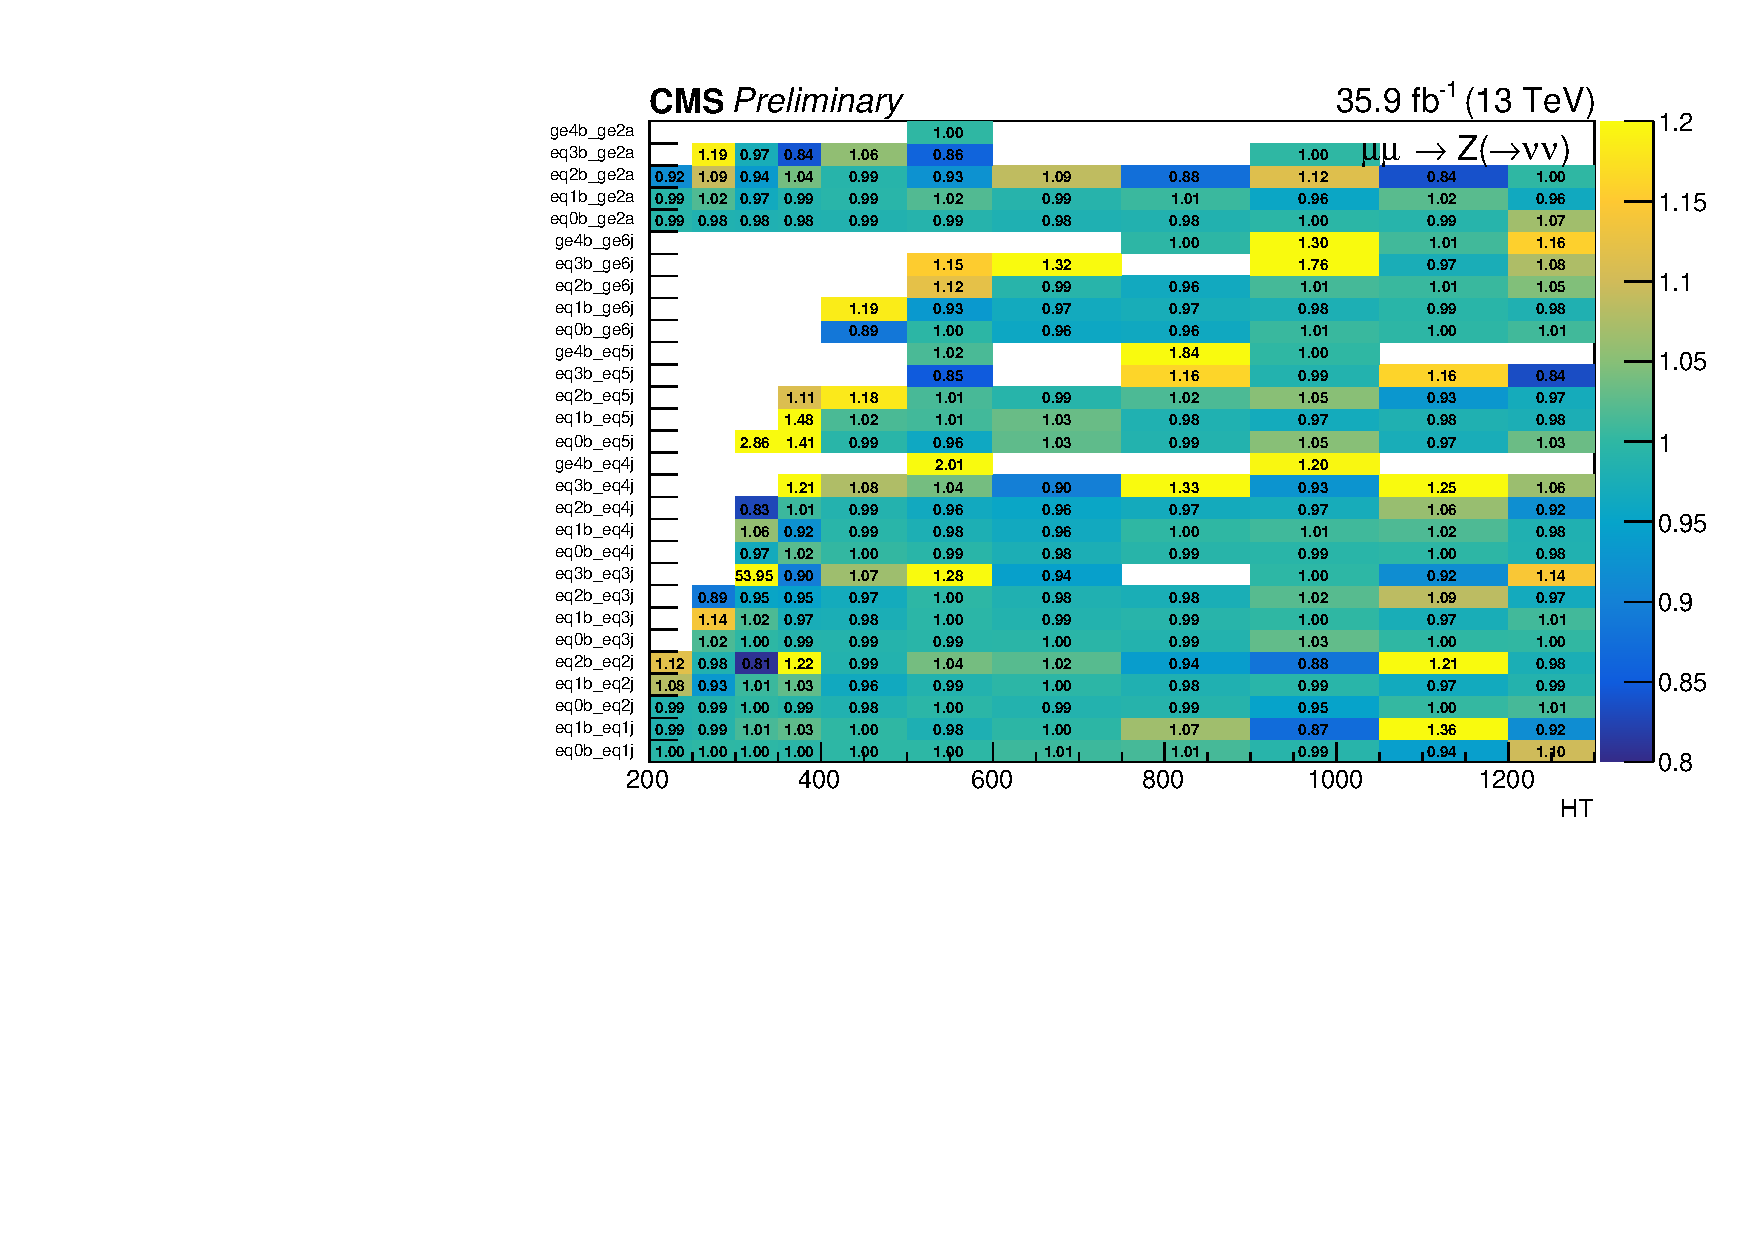
\includegraphics[width=0.5\textwidth]{figures/mcSystematics36p4fb/plots/tfratio_mumu_Zinv_2d_jecDown.pdf}
  }\\
  \subfigure[Up/down variations versus \njet.]{
    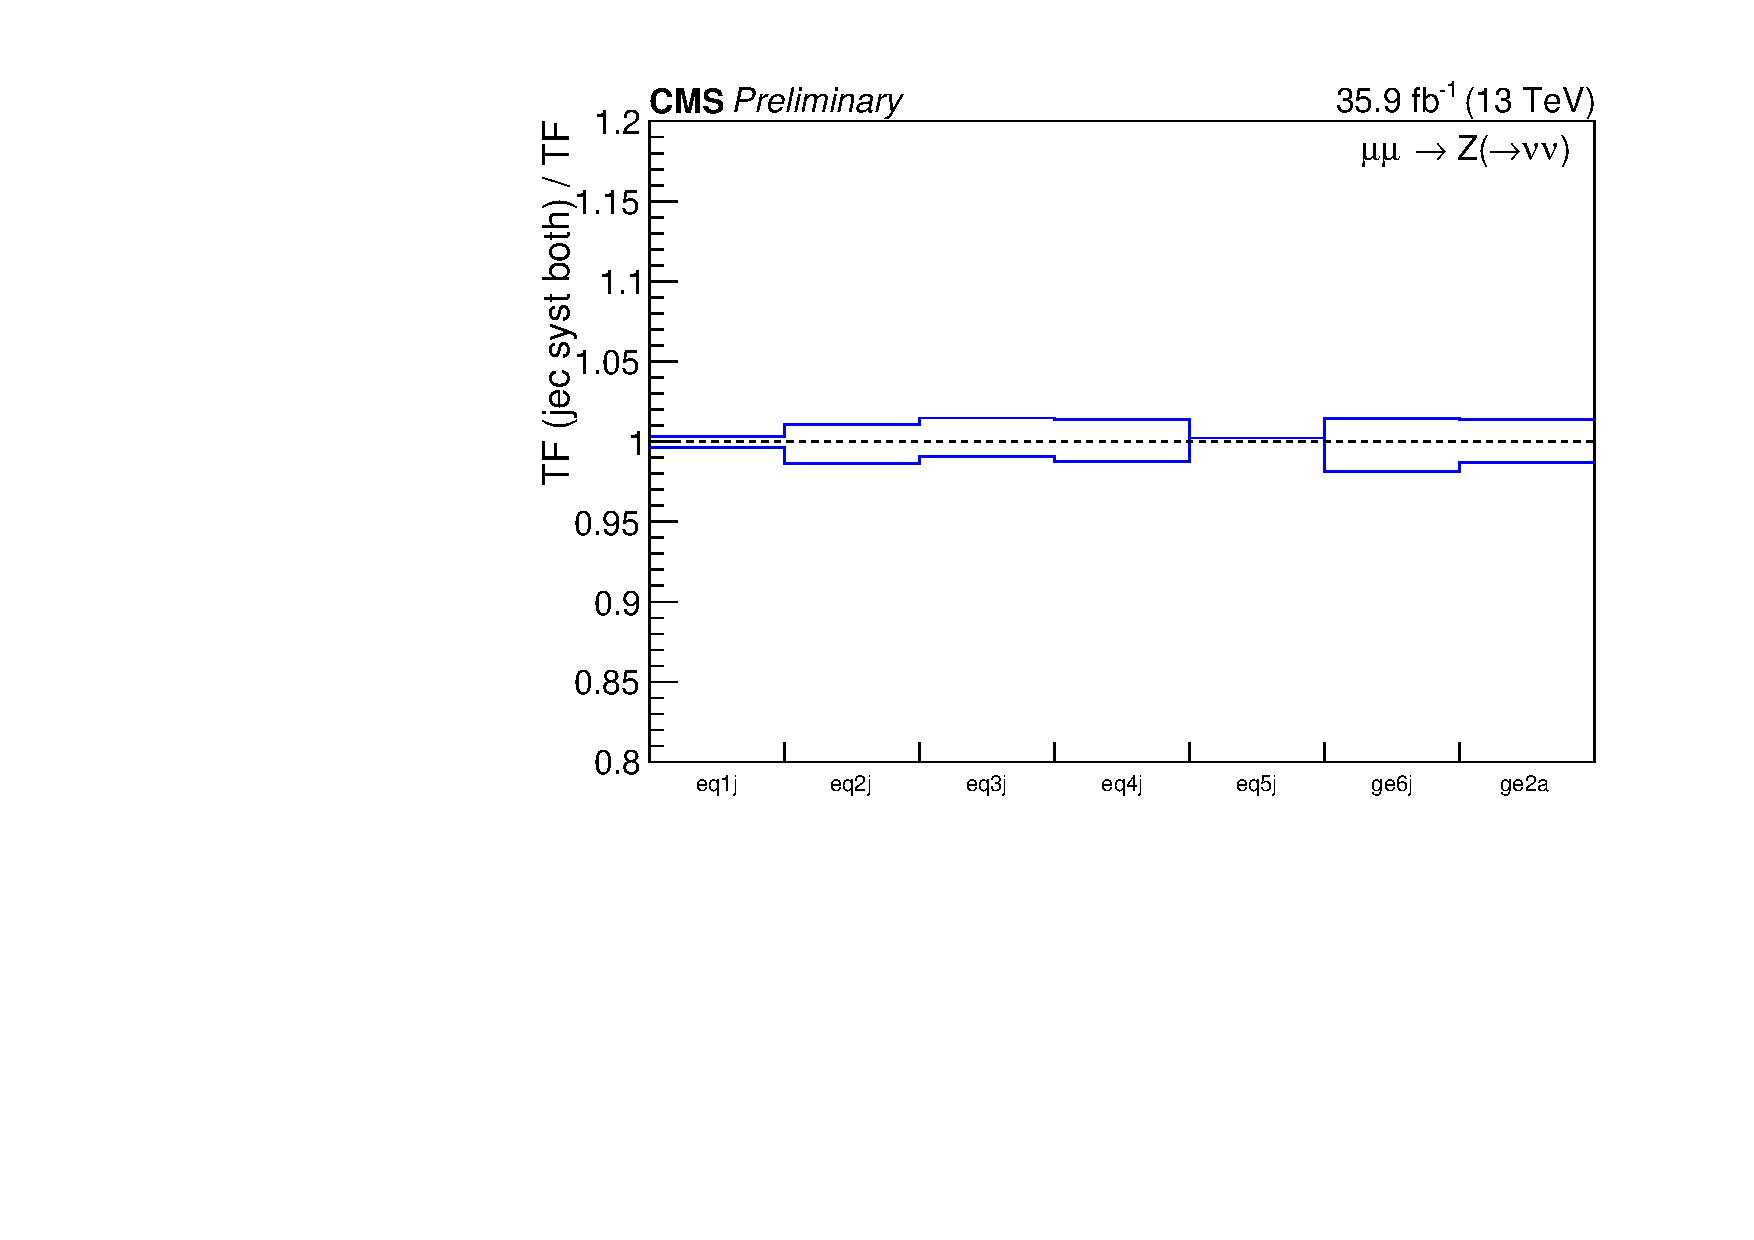
\includegraphics[width=0.5\textwidth]{figures/mcSystematics36p4fb/plots/tfratio_mumu_Zinv_njet_jecUp.pdf}
  } ~
  \subfigure[Up/down variations versus \scalht.]{
    \includegraphics[width=0.5\textwidth]{figures/mcSystematics36p4fb/plots/tfratio_mumu_Zinv_ht_jecUp.pdf}
  } \\
  \subfigure[Up/down variations versus \nb.]{
    \includegraphics[width=0.5\textwidth]{figures/mcSystematics36p4fb/plots/tfratio_mumu_Zinv_bjet_jecUp.pdf}
  } ~
  \subfigure[Up/down variations versus \mht.]{
    \includegraphics[width=0.5\textwidth]{figures/mcSystematics36p4fb/plots/tfratio_mumu_Zinv_mht_jecUp.pdf}
  } \\
  \caption{\label{fig:tfSyst_jec_mmZinv} The relative change in the
    ``$\mmj \rightarrow \znunu\ + \textrm{jets}$'' transfer factors from
    simulation due to $\pm1\sigma$ uncertainties in corrections to the
    jet energy scale.  }
\end{figure}

\clearpage
\subsection{B-tagging efficiency and mistag probability}

\begin{figure}[!h]
  \centering
  \subfigure[Up variation versus (\njet,\nb) category and \scalht.]{
    \includegraphics[width=0.5\textwidth]{figures/mcSystematics36p4fb/plots/tfratio_mumu_Zinv_2d_bsfWeightUp.pdf}
  } ~
  \subfigure[Down variation versus (\njet,\nb) category and \scalht.]{
    \includegraphics[width=0.5\textwidth]{figures/mcSystematics36p4fb/plots/tfratio_mumu_Zinv_2d_bsfWeightDown.pdf}
  }\\
  \subfigure[Up/down variations versus \njet.]{
    \includegraphics[width=0.5\textwidth]{figures/mcSystematics36p4fb/plots/tfratio_mumu_Zinv_njet_bsfWeightUp.pdf}
  } ~
  \subfigure[Up/down variations versus \scalht.]{
    \includegraphics[width=0.5\textwidth]{figures/mcSystematics36p4fb/plots/tfratio_mumu_Zinv_ht_bsfWeightUp.pdf}
  } \\
  \subfigure[Up/down variations versus \nb.]{
    \includegraphics[width=0.5\textwidth]{figures/mcSystematics36p4fb/plots/tfratio_mumu_Zinv_bjet_bsfWeightUp.pdf}
  } ~
  \subfigure[Up/down variations versus \mht.]{
    \includegraphics[width=0.5\textwidth]{figures/mcSystematics36p4fb/plots/tfratio_mumu_Zinv_mht_bsfWeightUp.pdf}
  } \\
  \caption{\label{fig:tfSyst_bsf_mmZinv} The relative change in the
    ``$\mmj \rightarrow \znunu\ + \textrm{jets}$'' transfer factors from
    simulation due to $\pm1\sigma$ uncertainties in the data/MC scale
    factors associated with b-quark tag efficiency.  }
\end{figure}

\clearpage
\begin{figure}[!h]
  \centering
  \subfigure[Up variation versus (\njet,\nb) category and \scalht.]{
    \includegraphics[width=0.5\textwidth]{figures/mcSystematics36p4fb/plots/tfratio_mumu_Zinv_2d_bsfLightWeightUp.pdf}
  } ~
  \subfigure[Down variation versus (\njet,\nb) category and \scalht.]{
    \includegraphics[width=0.5\textwidth]{figures/mcSystematics36p4fb/plots/tfratio_mumu_Zinv_2d_bsfLightWeightDown.pdf}
  }\\
  \subfigure[Up/down variations versus \njet.]{
    \includegraphics[width=0.5\textwidth]{figures/mcSystematics36p4fb/plots/tfratio_mumu_Zinv_njet_bsfLightWeightUp.pdf}
  } ~
  \subfigure[Up/down variations versus \scalht.]{
    \includegraphics[width=0.5\textwidth]{figures/mcSystematics36p4fb/plots/tfratio_mumu_Zinv_ht_bsfLightWeightUp.pdf}
  } \\
  \subfigure[Up/down variations versus \nb.]{
    \includegraphics[width=0.5\textwidth]{figures/mcSystematics36p4fb/plots/tfratio_mumu_Zinv_bjet_bsfLightWeightUp.pdf}
  } ~
  \subfigure[Up/down variations versus \mht.]{
    \includegraphics[width=0.5\textwidth]{figures/mcSystematics36p4fb/plots/tfratio_mumu_Zinv_mht_bsfLightWeightUp.pdf}
  } \\
  \caption{\label{fig:tfSyst_bsfl_mmZinv} The relative change in the
    ``$\mmj \rightarrow \znunu\ + \textrm{jets}$'' transfer factors from
    simulation due to $\pm1\sigma$ uncertainties in the data/MC scale
    factors associated with b-quark mistag probabilities.  }
\end{figure}

\clearpage
\subsection{Extrapolation in \texorpdfstring{\alphat}{AlphaT}}

\begin{figure}[h!]
  \begin{center}
    \includegraphics[width=0.45\textwidth]{figures/closureTests/AlphaT/DoubleMu_alphaTExtrapolation_ht.pdf}~
    \includegraphics[width=0.45\textwidth]{figures/closureTests/AlphaT/DoubleMu_alphaTExtrapolation_nJet.pdf}\\
    \caption{Data-driven closure tests probing the modelling of an
      extrapolation in the \alphat variable with the \mmj sample. The
      level of closure (solid markers) is indicated as a function of
      \scalht (left) and \njet (right). The blue histogram indicates
      the quadrature sum of the magnitude of non-closure and its
      statistical uncertainty. The post-fit closure (open markers) is
      also shown (see text for details).  }
    \label{fig:closure_AlphaT_mumu}
  \end{center} 
\end{figure}

%\begin{figure}[h!]
%  \begin{center}
%    \includegraphics[width=0.45\textwidth]{figures/closureTests/AlphaT/SinglePhoton_alphaTExtrapolation_ht.pdf}~
%    \includegraphics[width=0.45\textwidth]{figures/closureTests/AlphaT/SinglePhoton_alphaTExtrapolation_nJet.pdf}\\ 
%    \caption{As for Fig.~\ref{fig:closure_AlphaT_mu} but probing the
%      modelling of an extrapolation in the \alphat variable with the
%      \gj sample.
%    }
%    \label{fig:closure_AlphaT_phot}
%  \end{center} 
%\end{figure}

%\begin{figure}[h!]
%  \begin{center}
%    \includegraphics[width=0.45\textwidth]{figures/closureTests/AlphaT/AlphaT_Correlated_nuisances.pdf}
%    \caption{The post-fit nuisance parameter values (relative to
%      pre-fit) for the \alphat closure test when implemented as a
%      binned likelihood fit.} 
%    \label{fig:closure_AlphaT_LH_mu}
%  \end{center} 
%\end{figure}

\clearpage
\subsection{Extrapolation in \texorpdfstring{\bdphi}{biased dPhi}}

\begin{figure}[h!]
  \begin{center}
    \includegraphics[width=0.45\textwidth]{figures/closureTests/bDPhi/DoubleMu_bdphiExtrapolation_ht.pdf}~
    \includegraphics[width=0.45\textwidth]{figures/closureTests/bDPhi/DoubleMu_bdphiExtrapolation_nJet.pdf}\\
    \caption{Data-driven closure tests probing the modelling of an
      extrapolation in the \bdphi variable with the \mmj sample. The
      level of closure (solid markers) is indicated as a function of
      \scalht (left) and \njet (right). The blue histogram indicates
      the quadrature sum of the magnitude of non-closure and its
      statistical uncertainty. The post-fit closure (open markers) is
      also shown (see text for details).  }
    \label{fig:closure_bDPhi_mumu}
  \end{center} 
\end{figure}

%\begin{figure}[h!]
%  \begin{center}
%    \includegraphics[width=0.45\textwidth]{figures/closureTests/bDPhi/SinglePhoton_bdphiExtrapolation_ht.pdf}~
%    \includegraphics[width=0.45\textwidth]{figures/closureTests/bDPhi/SinglePhoton_bdphiExtrapolation_nJet.pdf}\\ 
%    \caption{As for Fig.~\ref{fig:closure_bDPhi_mu} but probing the
%      modelling of an extrapolation in the \bdphi variable with the
%      \gj sample.
%    }
%    \label{fig:closure_bDPhi_phot}
%  \end{center} 
%\end{figure}

%\clearpage
%\subsection{Extrapolation in \texorpdfstring{\alphat}{AlphaT} and
%  \texorpdfstring{\bdphi}{biased dPhi}}
%
%\begin{figure}[h!]
%  \begin{center}
%    \includegraphics[width=0.45\textwidth]{figures/closureTests/AlphaT_bDPhi/DoubleMu_alphaTbdphi_ht.pdf}~
%    \includegraphics[width=0.45\textwidth]{figures/closureTests/AlphaT_bDPhi/DoubleMu_alphaTbdphi_nJet.pdf}\\
%    \caption{Data-driven closure tests probing the modelling of an
%      extrapolation in both \alphat and \bdphi variables, as done in
%      the analysis, with the \mmj sample. The level of closure (solid
%      markers) is indicated as a function of \scalht (left) and \njet
%      (right). The blue histogram indicates the quadrature sum of the
%      magnitude of non-closure and its statistical uncertainty. The
%      post-fit closure (open markers) is also shown (see text for
%      details). \fixme{UPDATE PLOTS WITH CLOSURE FIT!} }
%    \label{fig:closure_AlphaT_bDPhi_mumu}
%  \end{center} 
%\end{figure}

%\begin{figure}[h!]
%  \begin{center}
%    \includegraphics[width=0.45\textwidth]{figures/closureTests/AlphaT/AlphaT_Correlated_nuisances.pdf}
%    \caption{The post-fit nuisance parameter values (relative to
%      pre-fit) for the combined \alphat and \bdphi closure test when
%      implemented as a binned likelihood fit. \fixme{UPDATE PLOT!!!}} 
%    \label{fig:closure_AlphaT_bDPhi_LH_mumu}
%  \end{center} 
%\end{figure}

\clearpage
\subsection{The single isolated track veto}

\begin{figure}[h!]
  \begin{center}
    \includegraphics[width=0.45\textwidth]{figures/closureTests/SITV/DoubleMu_Sit_ht.pdf}~
    \includegraphics[width=0.45\textwidth]{figures/closureTests/SITV/DoubleMu_Sit_nJet.pdf}\\
    \caption{Data-driven closure tests that probe the modelling of the
      single isolated track veto. The level of closure (solid markers)
      is indicated as a function of \scalht (left) and \njet
      (right). The blue histogram indicates the quadrature sum of the
      magnitude of non-closure and its statistical uncertainty. }
    \label{fig:closure_SITV_mumu}
  \end{center} 
\end{figure}

\clearpage
\subsection{Systematics uncertainties in the \texorpdfstring{\HTmiss}{MHT} templates}
\label{app:mht-zinv}

\begin{figure}[h!]
  \begin{center}
    \subfigure[$400 < \scalht < 500\GeV$]{\includegraphics[width=0.32\textwidth]{figures/mhtTemplate/exclusive/fits/MuMu/ht400_500_control_eq0b_eq2j_MuMu.pdf}}
    \subfigure[$500 < \scalht < 600\GeV$]{\includegraphics[width=0.32\textwidth]{figures/mhtTemplate/exclusive/fits/MuMu/ht500_600_control_eq0b_eq2j_MuMu.pdf}}
    \subfigure[$600 < \scalht < 750\GeV$]{\includegraphics[width=0.32\textwidth]{figures/mhtTemplate/exclusive/fits/MuMu/ht600_750_control_eq0b_eq2j_MuMu.pdf}}\\
    \subfigure[$750 < \scalht < 900\GeV$]{\includegraphics[width=0.32\textwidth]{figures/mhtTemplate/exclusive/fits/MuMu/ht750_900_control_eq0b_eq2j_MuMu.pdf}}
    \subfigure[$900 < \scalht < 1050\GeV$]{\includegraphics[width=0.32\textwidth]{figures/mhtTemplate/exclusive/fits/MuMu/ht900_1050_control_eq0b_eq2j_MuMu.pdf}}
    \subfigure[$1050 < \scalht < 1200\GeV$]{\includegraphics[width=0.32\textwidth]{figures/mhtTemplate/exclusive/fits/MuMu/ht1050_1200_control_eq0b_eq2j_MuMu.pdf}}\\
    \subfigure[$\scalht > 1200\GeV$]{\includegraphics[width=0.32\textwidth]{figures/mhtTemplate/exclusive/fits/MuMu/ht1200_Inf_control_eq0b_eq2j_MuMu.pdf}}
    \caption{The ratio of event yields obtained from data and simulation as a function of \mht [GeV] based on a sample of \mmj events that satisfy $\njet = 2$ and $\nb = 0$, as well as the requirements on \scalht indicated by each sub-figure caption. Also shown are fits to the ratios using first-order orthogonal polynomials.}
    \label{fig:mhtval_MuMu_eq2j_eq0b}
  \end{center}
\end{figure}

\begin{figure}[h!]
  \begin{center}
    \subfigure[$400 < \scalht < 500\GeV$]{\includegraphics[width=0.32\textwidth]{figures/mhtTemplate/exclusive/fits/MuMu/ht400_500_control_eq1b_eq2j_MuMu.pdf}}
    \subfigure[$500 < \scalht < 600\GeV$]{\includegraphics[width=0.32\textwidth]{figures/mhtTemplate/exclusive/fits/MuMu/ht500_600_control_eq1b_eq2j_MuMu.pdf}}
    \subfigure[$600 < \scalht < 750\GeV$]{\includegraphics[width=0.32\textwidth]{figures/mhtTemplate/exclusive/fits/MuMu/ht600_750_control_eq1b_eq2j_MuMu.pdf}}\\
    \caption{The ratio of event yields obtained from data and simulation as a function of \mht [GeV] based on a sample of \mmj events that satisfy $\njet = 2$ and $\nb = 1$, as well as the requirements on \scalht indicated by each sub-figure caption. Also shown are fits to the ratios using first-order orthogonal polynomials.}
    \label{fig:mhtval_MuMu_eq2j_eq1b}
  \end{center}
\end{figure}

\begin{figure}[h!]
  \begin{center}
    \subfigure[$400 < \scalht < 500\GeV$]{\includegraphics[width=0.32\textwidth]{figures/mhtTemplate/exclusive/fits/MuMu/ht400_500_control_eq0b_eq3j_MuMu.pdf}}
    \subfigure[$500 < \scalht < 600\GeV$]{\includegraphics[width=0.32\textwidth]{figures/mhtTemplate/exclusive/fits/MuMu/ht500_600_control_eq0b_eq3j_MuMu.pdf}}
    \subfigure[$600 < \scalht < 750\GeV$]{\includegraphics[width=0.32\textwidth]{figures/mhtTemplate/exclusive/fits/MuMu/ht600_750_control_eq0b_eq3j_MuMu.pdf}}\\
    \subfigure[$750 < \scalht < 900\GeV$]{\includegraphics[width=0.32\textwidth]{figures/mhtTemplate/exclusive/fits/MuMu/ht750_900_control_eq0b_eq3j_MuMu.pdf}}
    \subfigure[$900 < \scalht < 1050\GeV$]{\includegraphics[width=0.32\textwidth]{figures/mhtTemplate/exclusive/fits/MuMu/ht900_1050_control_eq0b_eq3j_MuMu.pdf}}
    \subfigure[$1050 < \scalht < 1200\GeV$]{\includegraphics[width=0.32\textwidth]{figures/mhtTemplate/exclusive/fits/MuMu/ht1050_1200_control_eq0b_eq3j_MuMu.pdf}}\\
    \subfigure[$\scalht > 1200\GeV$]{\includegraphics[width=0.32\textwidth]{figures/mhtTemplate/exclusive/fits/MuMu/ht1200_Inf_control_eq0b_eq3j_MuMu.pdf}}
    \caption{The ratio of event yields obtained from data and simulation as a function of \mht [GeV] based on a sample of \mmj events that satisfy $\njet = 3$ and $\nb = 0$, as well as the requirements on \scalht indicated by each sub-figure caption. Also shown are fits to the ratios using first-order orthogonal polynomials.}
    \label{fig:mhtval_MuMu_eq3j_eq0b}
  \end{center}
\end{figure}

\begin{figure}[h!]
  \begin{center}
    \subfigure[$400 < \scalht < 500\GeV$]{\includegraphics[width=0.32\textwidth]{figures/mhtTemplate/exclusive/fits/MuMu/ht400_500_control_eq1b_eq3j_MuMu.pdf}}
    \subfigure[$500 < \scalht < 600\GeV$]{\includegraphics[width=0.32\textwidth]{figures/mhtTemplate/exclusive/fits/MuMu/ht500_600_control_eq1b_eq3j_MuMu.pdf}}
    \subfigure[$600 < \scalht < 750\GeV$]{\includegraphics[width=0.32\textwidth]{figures/mhtTemplate/exclusive/fits/MuMu/ht600_750_control_eq1b_eq3j_MuMu.pdf}}\\
    \subfigure[$750 < \scalht < 900\GeV$]{\includegraphics[width=0.32\textwidth]{figures/mhtTemplate/exclusive/fits/MuMu/ht750_900_control_eq1b_eq3j_MuMu.pdf}}
    \caption{The ratio of event yields obtained from data and simulation as a function of \mht [GeV] based on a sample of \mmj events that satisfy $\njet = 3$ and $\nb = 1$, as well as the requirements on \scalht indicated by each sub-figure caption. Also shown are fits to the ratios using first-order orthogonal polynomials.}
    \label{fig:mhtval_MuMu_eq3j_eq1b}
  \end{center}
\end{figure}

\begin{figure}[h!]
  \begin{center}
    \subfigure[$400 < \scalht < 500\GeV$]{\includegraphics[width=0.32\textwidth]{figures/mhtTemplate/exclusive/fits/MuMu/ht400_500_control_eq0b_eq4j_MuMu.pdf}}
    \subfigure[$500 < \scalht < 600\GeV$]{\includegraphics[width=0.32\textwidth]{figures/mhtTemplate/exclusive/fits/MuMu/ht500_600_control_eq0b_eq4j_MuMu.pdf}}
    \subfigure[$600 < \scalht < 750\GeV$]{\includegraphics[width=0.32\textwidth]{figures/mhtTemplate/exclusive/fits/MuMu/ht600_750_control_eq0b_eq4j_MuMu.pdf}}\\
    \subfigure[$750 < \scalht < 900\GeV$]{\includegraphics[width=0.32\textwidth]{figures/mhtTemplate/exclusive/fits/MuMu/ht750_900_control_eq0b_eq4j_MuMu.pdf}}
    \subfigure[$900 < \scalht < 1050\GeV$]{\includegraphics[width=0.32\textwidth]{figures/mhtTemplate/exclusive/fits/MuMu/ht900_1050_control_eq0b_eq4j_MuMu.pdf}}
    \subfigure[$1050 < \scalht < 1200\GeV$]{\includegraphics[width=0.32\textwidth]{figures/mhtTemplate/exclusive/fits/MuMu/ht1050_1200_control_eq0b_eq4j_MuMu.pdf}}\\
    \subfigure[$\scalht > 1200\GeV$]{\includegraphics[width=0.32\textwidth]{figures/mhtTemplate/exclusive/fits/MuMu/ht1200_Inf_control_eq0b_eq4j_MuMu.pdf}}
    \caption{The ratio of event yields obtained from data and simulation as a function of \mht [GeV] based on a sample of \mmj events that satisfy $\njet = 4$ and $\nb = 0$, as well as the requirements on \scalht indicated by each sub-figure caption. Also shown are fits to the ratios using first-order orthogonal polynomials.}
    \label{fig:mhtval_MuMu_eq4j_eq0b}
  \end{center}
\end{figure}

\begin{figure}[h!]
  \begin{center}
    \subfigure[$500 < \scalht < 600\GeV$]{\includegraphics[width=0.32\textwidth]{figures/mhtTemplate/exclusive/fits/MuMu/ht500_600_control_eq1b_eq4j_MuMu.pdf}}
    \subfigure[$600 < \scalht < 750\GeV$]{\includegraphics[width=0.32\textwidth]{figures/mhtTemplate/exclusive/fits/MuMu/ht600_750_control_eq1b_eq4j_MuMu.pdf}}
    \subfigure[$750 < \scalht < 900\GeV$]{\includegraphics[width=0.32\textwidth]{figures/mhtTemplate/exclusive/fits/MuMu/ht750_900_control_eq1b_eq4j_MuMu.pdf}}\\
    \caption{The ratio of event yields obtained from data and simulation as a function of \mht [GeV] based on a sample of \mmj events that satisfy $\njet = 4$ and $\nb = 1$, as well as the requirements on \scalht indicated by each sub-figure caption. Also shown are fits to the ratios using first-order orthogonal polynomials.}
    \label{fig:mhtval_MuMu_eq4j_eq1b}
  \end{center}
\end{figure}

\begin{figure}[h!]
  \begin{center}
    \subfigure[$600 < \scalht < 750\GeV$]{\includegraphics[width=0.32\textwidth]{figures/mhtTemplate/exclusive/fits/MuMu/ht600_750_control_eq0b_eq5j_MuMu.pdf}}
    \subfigure[$750 < \scalht < 900\GeV$]{\includegraphics[width=0.32\textwidth]{figures/mhtTemplate/exclusive/fits/MuMu/ht750_900_control_eq0b_eq5j_MuMu.pdf}}
    \subfigure[$900 < \scalht < 1050\GeV$]{\includegraphics[width=0.32\textwidth]{figures/mhtTemplate/exclusive/fits/MuMu/ht900_1050_control_eq0b_eq5j_MuMu.pdf}}\\
    \subfigure[$\scalht > 1200\GeV$]{\includegraphics[width=0.32\textwidth]{figures/mhtTemplate/exclusive/fits/MuMu/ht1200_Inf_control_eq0b_eq5j_MuMu.pdf}}
    \caption{The ratio of event yields obtained from data and simulation as a function of \mht [GeV] based on a sample of \mmj events that satisfy $\njet = 5$ and $\nb = 0$, as well as the requirements on \scalht indicated by each sub-figure caption. Also shown are fits to the ratios using first-order orthogonal polynomials.}
    \label{fig:mhtval_MuMu_eq5j_eq0b}
  \end{center}
\end{figure}

\clearpage
\subsection{Era-dependent behaviour related to the \texorpdfstring{\nb}{Nb} modelling}
\label{app:nb-zinv}

Given the issues related to the ``HIP effect'' observed during the run
eras B-F of the 2016 data taking period, a dedicated study has been
performed to check the behaviour of the nuisances that encapsulate the
b-tag scale factor uncertainties. The BTV POG has provided
era-dependent scale factors (and uncertainties), covering eras B-F and
G-H independently. A binned likelihood fit to the data in the \mmj
sample is performed for the full data set and these two separate sets
of eras. The likelihood fit includes several other nuisances related
to known theoretical and experimental sources of uncertainty, as well
as those related to the b-tag scale factors for genuine tags of
b-quark jets (``bsf'') and mistag of light flavour (``bsfl'').

Unconstrained ``rate'' parameters are used per (\njet, \scalht) event
category to correct the simulation normalisation to data and the
simulation modelling of the \nb dimension in each (\njet, \scalht)
category is fit to data within the statistical uncertainties
associated with the data and smiulated counts. {\it Nota bene that the
  extrapolation from $\nb \geq 0$ is not done in the analysis, but
  this study demonstrates the effect of the era-dependent behaviour,
  which is mitigated by the subdivision of the \mmj event counts
  according to $\nb = 0$ and $\nb \geq 1$.} The systematic effects of
the b-tag scale-factor uncertainties are encapsulated by the two
nuisances ``bsf'' and ``bsfl'', which correlate each behaviour across
all (\njet, \scalht) event categories. Figure~\ref{fig:btagsf} shows
the post-fit nuisances for the three sets of run eras: full, B-F, and
G-H. The accuracy of the \nb modelling, following the application of
the (era-dependent) scale factor corrections, appears to depend on the
run era. 

It is noted here that Figure~\ref{fig:btagsf} (top) can be compared
directly with Figure~\ref{fig:btagsfge1b} (top) in
Sec.~\ref{sec:nb-zinv}, with the only difference being that the fit
reported in this section uses ``vanilla'' Monte Carlo counts to obtain
the \nb distriution, whereas the study in Sec.~\ref{sec:nb-zinv}
relies on the ``formula method'' described in Sec.~\ref{sec:formula}.

\begin{figure}[h!]
  \centering
  \includegraphics[width=0.6\textwidth]{figures/btag/nuisances/full/Correlated_nuisances}
  \includegraphics[width=0.6\textwidth]{figures/btag/nuisances/BF/Correlated_nuisances}
  \includegraphics[width=0.6\textwidth]{figures/btag/nuisances/GH/Correlated_nuisances}
  \caption{\label{fig:btagsf} Post-fit nuisances of a likelihood fit
    to data in the \mmj control region for (top) the full data set,
    (middle) run eras B-F, and (bottom) run eras G-H.}
\end{figure}

